%===============================================================================
%  Preamble
%===============================================================================
\documentclass[a4paper,10pt]{article}
\renewcommand{\thefootnote}{\roman{footnote}}
\usepackage[latin1]{inputenc}
\usepackage[dvips,pdftex]{graphicx}
\usepackage[small]{caption}  %Set text in Figure captions
\usepackage{parskip}         %does noindent in general and nice margin distance
\usepackage{fancyhdr}
\usepackage{subfigure}       %fix where figures go
\usepackage{amsmath}
\usepackage{courier}
\usepackage{longtable}       %fix long tables over various pages.
\usepackage{supertabular}
\usepackage{tabularx}        %fix long tables
\usepackage{multirow}        %fix nested tables
\usepackage{bigstrut}
\newcommand{\dirfig}{./pictures}
\usepackage{hyperref}
%\usepackage{gensymb}
%\usepackage{titlesec}
\pagestyle{fancy}
\usepackage[left=2.54cm,bottom=2.00cm,top=2.00cm,right=2.54cm]{geometry}
%Overrides all other setting to show what we want.
%\textwidth = 430pt \textheight = 640pt \voffset = -50pt
%\hoffset=-20pt
\usepackage{setspace}
\singlespacing
\setcounter{page}{0}
%\renewcommand{\thesection}{\Alph{section}}
%\usepackage[linktoc=all]{hyperref}
\hypersetup{
    colorlinks,
    citecolor=blue,
    filecolor=blue,
    linkcolor=blue,
    urlcolor=blue
}



%===============================================================================
%  Fonts in Document
%===============================================================================
%\usepackage{times}
%\usepackage{pslatex}
%\usepackage{newcent}
%\usepackage{palatcm}
%\usepackage{palatino}
%\usepackage[T1]{fontenc}
\usepackage[scaled]{helvet}
\renewcommand*\familydefault{\sfdefault}
%\renewcommand*{\encodingdefault}{T1}
% For more options go to: http://www.tug.dk/FontCatalogue/



%===============================================================================
% The document begins here with the title page
%===============================================================================
\begin{document}
\setcaptionmargin{0.5cm} %Fix caption margins
%\setlength{\oddsidemargin}{0.75in} % odd page left margin
%\setlength{\evensidemargin}{0.75in} % even page left margin
\thispagestyle{empty}
\begin{figure}[h]
\begin{center}
\resizebox{9cm}{!}{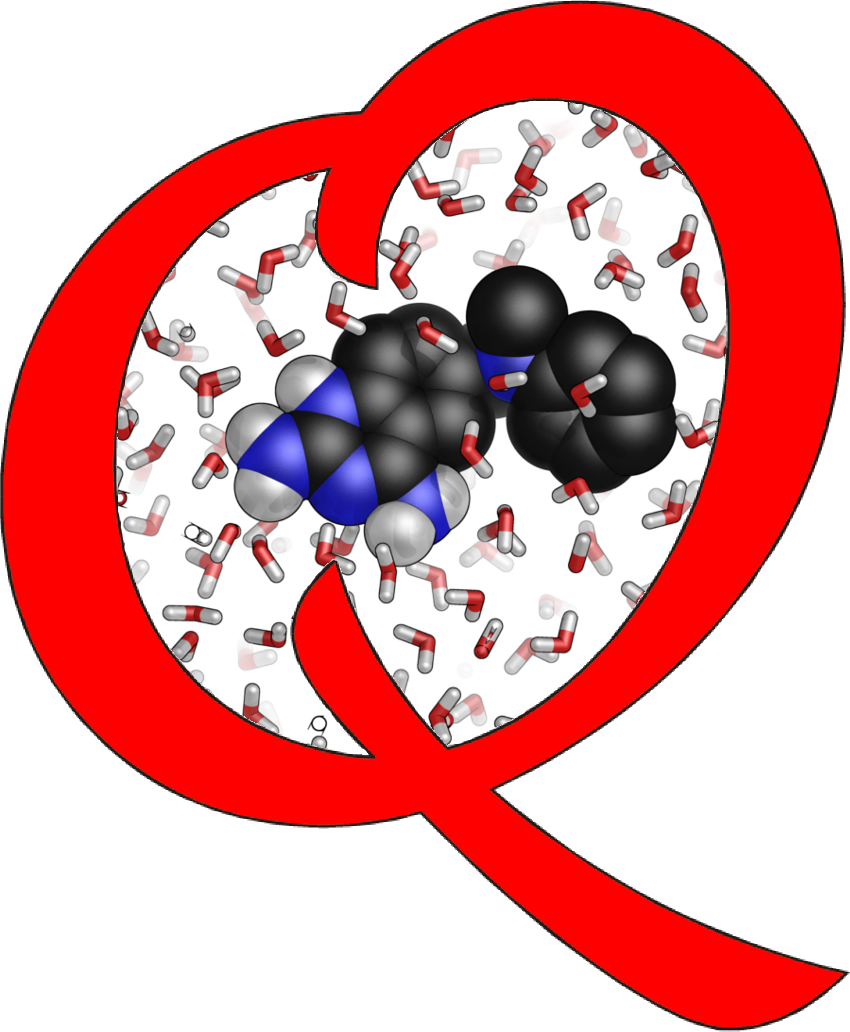
\includegraphics[scale=0.9]{\dirfig/qlogo.png}}
\end{center}
\end{figure}
\begin{center}
%\Huge{M}\huge{ANUAL}\\
%\huge{FOR}\\
%\huge{\textbf{our}} \Huge{M}\huge{OLECULAR} \Huge{D}\huge{YNAMICS}\\
%\huge{PACKAGE}\\% \Huge{Q}\\
\huge{\textbf{our}} 
{\fontsize{46}{46}\selectfont M}{\fontsize{30}{30}\selectfont OLECULAR}
{\fontsize{46}{46}\selectfont D}{\fontsize{30}{30}\selectfont YNAMICS}\\
\vspace{0.2cm}
{\fontsize{30}{30}\selectfont PACKAGE}
%\Huge{M}\huge{OLECULAR} \Huge{D}\huge{YNAMICS}\\
%\huge{PACKAGE}\\% \Huge{Q}\\




\vspace{8.0cm}
\Huge{Version 6.0.1}\\
\Huge{November 8, 2018}\\
%\footnotesize{February 6, 2015}\\
\vspace{0.8cm}
\large{\url{http://qdyn.no-ip.org/}}
\end{center}



%===============================================================================
% Table of contents
%===============================================================================
\newpage
\tableofcontents
\newpage



%===============================================================================
% Preface
%===============================================================================
\section{PREFACE}

\textbf{Q} started  its development sometime in  the nineteen nineties
originally by Johan \AA qvist, and  since then a list of collaborators
have  contributed  to  the  code, among  them:  John  Marelius,  Karin
Kolmodin,  Isabella Feierberg,  Martin  Alml\"of,  Martin Ander,  Jens
Carlson,  Peter  Hanspers,  Anders   Kaplan,  Kajsa  Ljunjberg,  Petra
Wennerstr\"om,  Martin Nervall,  Johan Sund,  Alexandre Barrozo,  Paul
Bauer, Beat  Amrein, Masoud Kazemi,  Irek Szeler, Miha  Purg, Mauricio
Esguerra and  \AA ke Sandgren. The  code is in active  development and
new features are  being implemented mainly following  the fortran 2003
standard.   Additionally the  MPI implementation  has been  updated to
enhance the speed  of running parallel jobs and provide  a more robust
parallelization across  different cluster architectures.   The program
code is  hosted online  thanks to a  generous github  academic account
granted to the program developers at Uppsala University.  Instructions
on  how to  obtain the  code  can be  found online  at the  Q-website:
\url{http://qdyn.no-ip.org/}.

Regarding the  name of the program  there are many conjectures  as the
original reason seems to be lost.  Maybe \textbf{Q} stands for
the commonly used letter to  describe partition functions, or maybe it
stands  for  the  letter  denoting  heat,  or  maybe  for  waiting  in
\textbf{Q}ueue, or perhaps it stands for charge, of  maybe for 
\textbf{Q}uantum, but we would be a bit hesitant about that last one.

The  molecule in  the  \textbf{Q}  logo is  that  of  a derivative  of
2,4-quinazolinediamine, to  be more  precise, its  full IUPAC  name is
6-[(N-methylanilino)methyl]quinazoline-2,4-diamine and  its pubchem id
is  CHEMBL78578. The  interest in  this molecule  comes from  it being
related to small molecules similar to quinine. Quinine was perhaps the
first effective  treatment against  malaria and it's  derivatives have
been researched  in the  pharmaceutical industry extensively  and have
also been part of the  research efforts\cite{Marelius:1998} at the \AA
qvist lab.


%===============================================================================
% Introduction
%===============================================================================
\section{INTRODUCTION}
Molecular  dynamics  (MD)  simulations  can  be  used  to  sample  the
thermally  accessible regions  of  conformational  space using  atomic
models of molecular systems.  From  the ensemble of sampled structures
and their associated  potential energies (given by the  force field or
molecular  mechanics  potential  energy  function)  it's  possible  to
compute  Gibbs  free  energies.    Quantities  such  as  binding  free
energies, solvation  free energies,  and activation free  energies are
particularly interesting  to compute because  they can be  obtained by
performing thermodynamic or kinetic  experiments.  It is thus possible
both to quantitatively verify  calculated results against experimental
data, and to make predictions which can be tested experimentally.

\textbf{Q}~\cite{Marelius:1999}   is   a   set   of   tools   tailored
specifically to compute free energies using diverse approaches, namely
(I)      free      energy     perturbation      (FEP)      simulations
\cite{Kollman:1993,Beveridge:1989}, (II) empirical  valence bond (EVB)
calculations   \cite{Warshel:1988,Aaqvist:1993}   of   reaction   free
energies    and     (III)    linear    interaction     energy    (LIE)
calculations\cite{Aaqvist:1994,Jones-Hertzog:1997,Hansson:1998}     of
receptor-ligand binding affinities.

The main features which distinguish  \textbf{Q} from other MD packages
are:
\begin{itemize}
\item \textbf{The spherical boundary.} \textbf{Q} is intended for free
  energy calculations in biomolecular  systems solvated in a spherical
  droplet  of explicit  water molecules.   Using a  spherical boundary
  \cite{Warshel:1978,Berkowitz:1982,Brunger:1984} makes it possible to
  limit  the  size  of  the  simulated system,  $i.e.$  to  focus  the
  simulation on  a smaller  region such  as a  binding site,  and also
  makes  accurate   treatment  of  long-range   electrostatics  rather
  inexpensive.
\item \textbf{The  flexibility in choice  of force field.}   The force
  fields are defined in parameter files, separate from the program and
  the choice of force field is thus simply a matter of which parameter
  file to use.
\item \textbf{The  ease of use  and learning.} The  simulation control
  input and force  field definition files are organized  in a flexible
  way and easy to understand  and modify.  The programs give extensive
  diagnostics when problems are encountered.
\item  \textbf{It runs  on any  computer and  simulates any  number of
  particles.}   By  using  dynamic memory  allocation  \textbf{Q}  can
  simulate biomolecules  of moderate size  on a personal  computer, or
  very  large  molecular  systems  on a  super-computer,  without  any
  modifications of the program.
\end{itemize}

The main features  which have been added to the  \textbf{Q} code since
version 5.0 are:

\begin{itemize}
\item \textbf{Periodic boundary conditions.} The periodic boundary
allows an additional way to perform calculations.

\item \textbf{Parallel version.} By using more than one computer a
single simulation can be executed faster. The parallel version is
especially useful when simulating large systems, $e.g.$ the
systems that are used with the periodic boundary condition.
\end{itemize}



%===============================================================================
% Installation and Setup
%===============================================================================
\section{INSTALLATION AND SETUP}
\subsection{System requirements} 
\textbf{Q}  can  be compiled  and run  in Windows  10, Mac  OSX and
Linux.   The  parallel \textbf{qdynp}  version  of  the main  dynamics
program \textbf{qdyn} has  been greatly improved from  that of version
5.0 which was using an  older Message Passing Interface (MPI) standard
and  one-sided communication  instead of  the more  portable point  to
point communication.

The memory requirements vary with the size of the simulated system but
are, in general, modest.  A system of  18 \AA ~radius with a cutoff of
10 \AA ~in non-bonded interactions uses about  3 to 7 Mb of RAM memory
depending slightly on the computer and operating system.

\subsubsection{Compilers} 
A  modern Fortran  compiler is  required  to build  the main  programs
(\textbf{qdyn},   \textbf{qprep},   \textbf{qfep},   \textbf{qdum}   ,
\textbf{qcalc}).

A  Fortran compiler  and  an  MPI library  is  required  to build  the
parallel version of \textbf{qdynp}.

\subsection{Installation}
The following components, available from the \textbf{Q} web site
\url{http://qdyn.no-ip.org}, are required to use \textbf{Q}:
\begin{enumerate}
\item Executable images (available for some popular platforms).
\item Or source code (to compile on your own system).
\item Force field parameter and library files.
\end{enumerate}
Create a folder (mkdir) such as $\sim$/software/q,  or C:$\backslash$q
and download the files to this directory, or clone them from the
github repository.

\subsubsection{Installing executable images}
\textbf{Windows 10}

\textbf{Linux}

\textbf{Mac OSX}

\subsubsection{Building the programs from source code}
\textbf{Windows 10}

\textbf{Linux} 

\textbf{Mac OSX}



%===============================================================================
% Main user guide.
%===============================================================================
\section{USER GUIDE}
The structure of \textbf{Q} resembles that of many other MD simulation
programs.  The main program which  solves Newton's equations of motion
(i.e., the  trajectory calculations) is called  \textbf{qdyn}. Besides
from input control  data, it needs a type of  data usually referred to
as molecular topology. This is a file containing information about how
atoms are bonded  to each other etc. together with  all the parameters
of the  force field (FF)  to be used.   This topology file  is created
with the  preparation program  \textbf{qprep} which is  an interactive
program that  uses pdb (Protein  Data Bank) coordinate  files together
with FF  specific files to  generate the topology.  \textbf{qprep} can
also  be  used  for  various other  data  transformation  purposes  as
described below.  Input  data for FEP, EVB  or receptor-ligand complex
simulations is given in a separate  file, referred to below as the fep
file. The fep  file lists atoms to be transformed,  called Q-atoms and
force  field  parameters  for  the different  states  in  perturbation
simulations.  For  analysis  of  the computations  the  main  tool  is
\textbf{qfep}  which  is  a  program  that carries  out  FEP  and  EVB
calculations  of   free  energies   using  energy  data   produced  by
\textbf{qdyn}.  A number  of utility  programs (trajectory  and energy
averaging, radial distribution functions,  ...) are also provided. The
general outline of \textbf{Q} is shown in figure \ref{fig:overview}.

\begin{figure}[h]
\begin{center}
\resizebox{15cm}{!}{\includegraphics*{\dirfig/Q_overview_2.pdf}}
\caption{Overview of the procedure for free energy calculation
with Q. The white boxes represent files and also show typical file
name extensions. The black boxes are programs.}
\label{fig:overview}
\end{center}
\end{figure}

In the  following sections we will  go through the normal  sequence of
steps  for preparing  a  topology file  with  \textbf{qprep} and  then
describe in detail the input  data required for running MD simulations
with \textbf{qdyn}.

\subsection{Preparing a molecular topology} The topology file
prepared with the program \textbf{qprep} contains all the information about
the molecular system needed for a simulation with \textbf{qdyn}. To make a
topology you need

\begin{itemize}
\item A molecular fragment library file describing the atoms and connectivity
of each protein residue, ligand etc., collectively referred to as
library entries.
\item A force-field parameter file.
\item Coordinates for all (non-solvent) atoms in the form of a PDB file.
\end{itemize}

\subsubsection{\textbf{qprep} - Preparing coordinates}
The  PDB  file  format  \cite{pdb}   used  for  coordinate  input  to
\textbf{qprep} is a fixed format, $i.e.$, the number of spaces between
columns  of   data  is   significant  and   tab  characters   are  not
permitted.  Case is  significant -  lower-case letters  should not  be
used. Only  ATOM and  HETATM records are  read by  \textbf{qprep}, all
other records are ignored.

Hydrogen atoms are not required  - their coordinates will be generated
by  \textbf{qprep} in  such a  way  that the  bond and  angles to  the
hydrogen  atom  are at  an  energy  minimum.  To further  control  the
placement of  hydrogens, a  special torsion  potential defined  in the
fragment library entry may be included. See [\textbf{build\_rules}] on
page \pageref{tab:buildrules}. If hydrogen  atom coordinates are given
in the PDB file, they will not be altered.

When  a structure  containing more  than one  molecule is  loaded into
\textbf{qprep},  the  program  will identify  the  boundaries  between
molecules either by the type of fragment or by placing a line with the
`GAP' keyword between molecules.   Fragments which constitute monomers
in  a polymer  chain, like  amino  acids, have  designated `head'  and
`tail' atoms  in their  library entries, defining  how they  should be
connected to  the neighbouring  residues.  Library  entries describing
separate  molecules such  as solvent  or ligands  do not  contain this
linkage  information.  To  distinguish  two peptide  chains from  each
other it is necessary  to introduce a gap marker line  in the PDB file
after the last atom of the first molecule.  The gap marker consists of
the word GAP in capital letters on a separate line.

The  numbering of  atoms  in the  PDB is  not  significant. Note  that
\textbf{qprep} will renumber  all atoms in a  single sequence starting
at one.  This is necessary in  order to incorporate hydrogen  atoms in
the sequence. The result is  that \textit{atom numbers in the PDB
  file   read   by  \textbf{qprep}   and   PDB   files  generated   by
  \textbf{qprep} will  be different}. Residue numbers  are used merely
to distinguish one residue from the next and the residues will also be
renumbered  by  \textbf{qprep}.  Residue   numbers  must  be  numeric,
alphanumeric  identifiers such  as  60A sometimes  encountered in  the
protein data bank are not permitted.

Protein structures  determined by  X-ray crystallography  are normally
refined  with  a  large  number  of water  molecules.  Some  of  these
well-ordered water  molecules may be  important for the  structure and
function   of   the   protein   and  should   be   included   in   the
simulation. However,  most of the crystallographic  waters surrounding
the protein can be removed. In fact, the presence of a large number of
water molecules around the protein  surface will disturb the solvation
algorithm  leading  to   inhomogenous  water  density.  \textbf{qprep}
assumes that  solvent molecules appear  after solute molecules  in the
PDB file and  keeps track of the last solute  atom.  Solvent molecules
are identified  by their  residue names. The  list of  solvent residue
names  is a  user-setable  preference in  \textbf{qprep} (see  Setting
preference on page \pageref{setting_pref}) with the default value WAT,
HOH,  H2O,  SPC,  TIP3.  Solvent  molecules  added  by  the  solvation
algorithm  will  appear at  the  end  of  the atom  sequence.  Solvent
molecules  outside the  simulation sphere  (more than  water radius  +
2~{\AA}  from  solvent centre)  will  be  excluded like  solute  atoms
outside the solute sphere.


\subsubsection{Selecting a force field}
\textbf{Q} is designed  to run with a wide selection  of force fields.
Fragment libraries and force field parameters for AMBER95, AMBER/OPLS,
OPLS-AA, CHARMM v.22, CHARMM v. 36, GROMOS87 and GROMOS96 are supplied
with the program. The corresponding library and FF parameter files are
listed in table \ref{tab:FF} on page \pageref{tab:FF}.  In addition to
all  the interaction  parameters, a  \textbf{Q} force  field parameter
file also includes overall properties of  the force field, such as the
van der Waals  equation parameter combination rule.  Selecting a force
field is thus  equivalent to loading the  appropriate fragment library
and parameter file into \textbf{qprep}.


\subsubsection{Adding force field library entries}
Your simulations will probably  include molecular fragments other than
the amino acid residues and solvent molecules that are included in the
standard library files and you therefore need to write a library entry
for  each  'new' residue,  ligand,  co-factor  or other  molecule.  We
suggest you keep  your library entries in a separate  file rather than
adding to the standard library  file.  Load first the standard library
and then your own into \textbf{qprep}.  If you need to modify an entry
in  the standard  library, add  the modified  entry (keeping  the same
name) to your  own library file -  it will replace the  old entry when
loaded.

The best starting point for generating a new entry is to copy an
old one, this ensures the correct syntax. For details, see the
section Fragment library file format on page
\pageref{subsubsec:fragment_lib_f_f}.


\subsubsection{Running \textbf{qprep}}
\textbf{qprep}  is  a  command-oriented  program designed  to  be  run
interactively. The first thing you  need to learn about \textbf{qprep}
is  that there  is a  help  command which  gives a  list of  available
commands. The  program's input parser  will prompt for  the parameters
required for each  command but will also accept  complex command lines
including  the parameters.  Thus,  you may  either  enter the  command
\textbf{readlib} and await  the prompt 'Name of  molecular library' or
you may type \textbf{readlib my{\_}ligands.lib} on one line.

A good  deal of effort  has been  spent to make  \textbf{qprep} handle
errors  gracefully.  When  a  problem is  encountered  in  a  fragment
library, parameter  file or  PDB file,  you will  be notified  but the
processing of the  file will proceed, thus exposing  also errors later
in the  file. After correcting  the problem  you simply read  the file
again without the need to restart the program.

The different  steps to  generate a  topology with  \textbf{qprep} are
described  below, in  the sequence  they are  normally executed.  More
detailed information is available  in the section Topology preparation
reference on page \pageref{subsec:top_prep_ref}.

\textbf{Loading fragment libraries}\\*
[0.25cm] Use the \textbf{readlib}  command to load fragment libraries.
Many libraries may be loaded by repeating the \textbf{readlib} command
for each of them.  Note that if one entry name  occurs more than once,
the latest  definition takes precedence.  A warning message  is issued
when a library entry is overloaded.

Errors encountered while reading a library will be displayed and after
they have been corrected, the library  may be loaded again.  To remove
all library entries from memory, use the \textbf{clearlib} command.

\textbf{Loading force field parameters}\\*
[0.25cm]  Use  the  \textbf{readprm  } command  to  load  force  field
parameters. As  opposed to  the case with  fragment libraries,  only a
single  parameter file  can  be  loaded. If  you  need  to modify  the
parameter  file,  edit and  save  it  and load  it  again.  It is  not
necessary to reload fragment libraries or the structure.

\textbf{Loading coordinates}\\*
[0.25cm]  Use  the  \textbf{readpdb}  command to  load  the  molecular
structure file.  Before loading the structure, the program will verify
that all the  required library entries are loaded and  that the number
of  heavy atoms  of each  fragment is  correct. Only  one file  can be
loaded   -  reading   another  file   clears  the   previously  loaded
structure. This is useful as you reload the same file after correcting
a problem.

\textbf{Choosing boundary condition}\\*
[0.25cm]  Use  the  \textbf{boundary}  command  to  set  the  boundary
condition; sphere or  box. When a boundary has been  chosen the centre
and radius  in the  spherical case, and  boxlengths in  the periodical
case  are  specified. It  is  important  that the  boundary  condition
defined in the topology file is consistent with the boundary condition
used when running dynamics with \textbf{qdyn}.

\textbf{Adding solvent}\\*
[0.25cm] Use the \textbf{solvate} command  to add solvent molecules to
the loaded structure. When using  a spherical boundary the solvent can
be generated by any of the following methods:

\begin{itemize}
\item Using  randomly oriented molecules  on a grid. This  option does
  not  depend on  any  solvent  coordinate file  but  only asks  which
  library  entry should  be  used.  The density  is  specified in  the
  library  entry.   The  sphere  center  can  be  specified  by  x,y,z
  coordinates,    residue\_number:atom\_name,   using    the   keyword
  \textit{MASS} to  center at the center  of mass of the  molecule, or
  using the  keyword \textit{BOUNDARY},  to use  the same  boundary as
  that which must have been given previously with the \textit{boundary}
  command. 
\item By reading solvent coordinates  from a solvent file. The solvent
  file  is similar  to a  PDB file,  see Solvent  file format  on page
  \pageref{subsubsec:solvent_file_format}.  The solvent  file contains
  coordinates for a sphere or box of solvent. In the case of a box, it
  will be replicated in all directions  as needed and can thus be used
  to solvate a system of any size.
\item  By reading  solvent  coordinates  from a  restart  file from  a
  previous simulation of the same molecular system.
\end{itemize}

When using one of the two  first methods, \textbf{qprep} first fills a
sphere completely with solvent and  then deletes molecules where heavy
atoms are  closer than a threshold  distance to any heavy  atom in the
loaded  structure.  The  threshold   distance  is  controlled  by  the
\textbf{qprep}     preference      value     \textbf{solvent{\_}pack}.
Crystallographic solvent molecules (in the PDB file loaded by readpdb)
more than 2~{\AA} outside the solvent sphere will be excluded from the
simulation to avoid excessive radial restraining forces.

If periodic boundary is used it is  not possible to use a solvent file
with  a sphere  of solvent.  Moreover the  threshold distance  is also
applied  to solvent  molecules  near the  boundary,  to avoid  crashes
between solvent molecules in neighbouring boxes.

At present, the  choice of solvent is limited  to tri-atomic molecules
like the SPC\cite{Berendsen:1981} and TIP3P\cite{Jorgensen:1983} water
models or methanol in an extended atom representation.

Note: Make sure that crystallographic water molecules and waters added
by the solvate command have \textit{the same residue name}!  Otherwise
\textbf{qprep} will mark  the topology as mixed-solvent,  which is not
implemented in \textbf{qdyn} at present.

\textbf{Adding cross-link bonds}\\*
[0.25cm] Cross-link bonds  such as disulphide bridges  in proteins are
not generated automatically {\-} they  are not defined in the fragment
library.  Extra bonds  can  be added  automatically  by searching  the
solute molecules for  close but not bonded atom pairs,  or manually by
specifying atom numbers.  To  generate cross-link bonds automatically,
use the  \textbf{xlink} command. For  each close atom pair  found, you
need to confirm or reject the making of a bond. To add bonds manually,
use the \textbf{addbond} and specify the atoms to be bonded, either by
atom numbers or in the form residue{\_}number:atom{\_}name.

\textbf{Generating the topology}\\*
[0.25cm] The \textbf{maketop}  command is used to  create the topology
in  memory.  The  only input  for  this  command  is  a name  for  the
topology.  The process  involves  the following  steps  which are  all
carried out by the maketop routine without further user input:

\begin{itemize}
\item Setting atom types and partial charges.
\item Generating the lists of bonds, bond angles, torsion angles and improper torsions.
\item Generating the neighbour exclusion and 1-4 neighbour lists.
\item Generating coordinates for hydrogen atoms not included in the loaded structure.
\item Marking atoms outside the simulation sphere as excluded
\item Calculation of the `effective solvent radius' used in the
simulation to ensure correct density of the solvent. This radius
which is based on the number and spatial distribution of solute
and solvent atoms in the sphere, typically differs somewhat from
the radius used in the solvation step.
\end{itemize}

\textbf{Verifying the topology}\\*
[0.25cm] The successful generation of a  topology in the step above is
no guarantee that  it is correct. Fortunately  \textbf{qprep} offers a
number of commands to check the topology:

\begin{itemize}
\item \textbf{Checkbonds} is used to list bonds with a potential energy
exceeding a specified threshold. This helps to identify errors in
the connectivity.
\item \textbf{Checkangs} lists angles with energies over a threshold.
\item \textbf{Checktors} lists torsion angles with energies over a threshold.
\item \textbf{Checkimps}  lists high energy improper torsion angles. This is
a very important step for users of force fields with harmonic
improper potentials (GROMOS, charmm) since with a non-periodic
potential it makes a huge difference if the angle is $e.g.$
-179$^{o}$ instead of +179$^{o}$ if the (single) energy minimum is
at +180$^{o}$ although the structural difference is small.
\textit{Impropers with the wrong sign give rise to high energies
and strong forces which will distort the molecule during the
simulation and must be corrected.} (This is not a problem with
periodic improper torsion potentials used in the other force
fields.) The sign of the angle depends on the order of the bonds
in the fragment library entry, each permutation of the sequence of
the bonds involved will change the sign of the angle. Instead of
modifying library entries, reloading the libraries and remaking
the topology, the \textbf{changeimp} command can be used to flip
the sign of selected impropers or of all impropers with energy
exceeding a threshold value.
\end{itemize}

\textbf{Writing topology and coordinate files}\\*
[0.25cm] The final step in making a topology is saving it to a file by
using the \textbf{writetop} command.

You will also need to make a PDB (or mol2, see below) file from
the topology to see the new numbers of the atoms. These are the
atom numbers you need to refer to when setting up restraints and
topology modifications for perturbation simulations. Use the
\textbf{writepdb} command to write a PDB file containing all the
atoms of the topology.

\textbf{Setting preferences}\label{setting_pref}\\*
[0.25cm]  A  number  of  parameters   that  affect  the  operation  of
\textbf{qprep}, $e.g.$  during solvation,  but which are  not normally
changed are  not required as  input to the commands.  These parameters
may  be changed  by experience  users by  the preference  mechanism in
\textbf{qprep}.

The \textbf{prefs} command is used to list the values of
user-setable parameters and the \textbf{set} command to change a
value.

The preference parameters and their default values are listed in
the table on page \pageref{subsubsec:Qprep_preferences}.

\subsection{Running dynamics with \textbf{qdyn}}
Once a molecular topology file has been generated with \textbf{qprep}, you
can carry out MD, FEP and EVB simulations with \textbf{qdyn}. The
simulation can have either spherical or periodic boundary
condition, and can be executed either sequentially or in parallel.

In this section we will describe the basic functions of \textbf{qdyn} and
go through the different options that are available for control of
the dynamics runs. There are two main input files that are used to
set up the dynamics specifications:

\begin{enumerate}
\item The \textbf{qdyn} input file that controls things like time-step, temperature,
cut-offs, restraints etc. \item The FEP file which is an auxiliary
file whose function is to redefine the topology information for
certain atoms. This enables the explicit control over selected
force field parameters that is necessary for FEP and EVB
calculations.
\end{enumerate}

\subsubsection{Simulation procedure}
The MD simulation required for a free energy calculation often
proceeds in multiple stages. Normally, the initial stage is run at
a very low temperature with strong coupling to the temperature
bath (similar to energy minimisation) to relax strain in the
initial structure. Then may follow stepwise heating of the
simulated system and equilibration for some time at the target
temperature. After this comes the main simulation during which
energy and structure data is collected. For perturbation
simulations, this phase is composed of a series of simulations
using intermediate potentials defined by different sets of weight
coefficients for the FEP states.

A separate \textbf{qdyn} input file is used for each sub-simulation. It is
therefore practical to prepare a command file (shell script or
batch file) which executes all the sub-simulations sequentially.
The name of the input file is passed to \textbf{qdyn} as the first (and
only) argument on the command line. (It is not possible to use
redirection of the standard input stream by the $<$ operator.) A
simple example of such a file where \textbf{qdyn} is invoked once for each
input file and the output redirected to a log file follows:

\begin{table}[htbp]
\begin{center}
\caption{Multi-stage simulation command file}
\begin{tabularx}{\textwidth}{|l l l X|}
  \hline
  \textbf{qdyn} & relax.inp & $>$ & relax.log \\
  \textbf{qdyn} & eq1.inp   & $>$ & eq1.log \\
  \textbf{qdyn} & eq2.inp   & $>$ & eq2.log \\
  \textbf{qdyn} & eq3.inp   & $>$ & eq3.log \\
  \textbf{qdyn} & data1.inp & $>$ & data1.log \\
  \textbf{qdyn} & data2.inp & $>$ & data2.log \\ \hline
\end{tabularx}
\end{center}
\end{table}

\subsubsection{Output generated by \textbf{qdyn}} The different data files
generated by \textbf{qdyn} are (shown in the overview in
\figurename~\ref{fig:overview}):

\begin{itemize}
\item General information about the progress of the simulation including
energy summaries and temperature is written to the standard output
device and normally redirected to a log file.
\item Final coordinates and velocities are written to a `restart' file to be
used to start the next sub-simulation and, after conversion to a
structure file (see Analyzing structures from the simulation on
page \pageref{subsubsec:Analyzing_struc_f_t_sim}, for viewing the
final structure. This file is also updated during the simulation
and if the forces and velocities become too large and the
simulation is terminated prematurely. The file thus also serves a
diagnostic purpose.
\item Energy data for Q-atoms in each FEP state is written to an
energy file every few time steps (determined in the input file).
\item Coordinates for all or a subset of atoms are written to a trajectory
file at regular intervals (determined in the input file).
\end{itemize}

The restart and energy files are Fortran binary files. The
trajectory file follows the DCD format also used in other MD
programs (Charmm, X-plor) and can be read by many visualization
and trajectory animation programs.

\subsubsection{Preparing \textbf{qdyn} input files}\label{subsubsec:prep_qdyn_inp_f}
In this overview the various aspects of defining the simulation
set-up are introduced. For more complete information, see \textbf{qdyn}
input file format on page \pageref{subsubsec:qdyn_inp_file_form}.

The \textbf{qdyn} input file contains the specification of the dynamics
simulation. It is a text file divided into sections, starting with
a section heading and containing information on the different
aspects of the simulation. The sections are of two kinds:

\begin{itemize}
\item Sections where each line consists of a keyword and a values, with
different keywords on each line.
\item Sections where all the lines
have the same formatting and together constitute a data set. No
keywords are used here.
\end{itemize}

Only a few sections are mandatory, most are optional and they may
appear in any order. The formatting within a section is flexible
in that blank lines are permitted as well as comments (starting
with !, {\#} or *) at the end of lines or on separate lines. The
format of the data in each record within a section is free (white
space is not significant), but all data in the record must be on
the same line.The units used are based on {\AA}, K and kcal/mol
(see Units on page \pageref{subsec:units}).

\bigskip
\textbf{Dynamics control information}\\*[0.25cm] The section
[\textbf{MD}] is normally the first in the input file the most
apparently required section, since it defines the core parameters
of the simulation like the number of time steps, their size and
the temperature. Below is an example of a basic MD section in an
input file:

\begin{center}
\begin{tabularx}{\textwidth}{|l X|}
  \hline
  [MD]             & \\
  steps            & 10000 \\
  stepsize         & 2.0 \\
  temperature      & 300 \\
  shake{\_}solvent & on \\
  shake{\_}solute  & off \\
  lrf              & on \\ \hline
\end{tabularx}
\end{center}

\bigskip
\textbf{Periodic boundary conditions}\\*[0.25cm] The
[\textbf{PBC}] section contains options and settings for
simulations with periodic boundary. The mere existence of the
section header [\textbf{PBC}] is enough to indicate the boundary
condition. Additional options is added as exemplified below:

\begin{center}
\begin{tabularx}{\textwidth}{|l X|}
  \hline
  [PBC]                  & \\
  rigid{\_}box{\_}centre & on \\
  constant{\_}pressure   & on \\
  max{\_}volume{\_}displ & 65 \\
  pressure               & 1.5 \\ \hline
\end{tabularx}
\end{center}

The rigid{\_}box{\_}centre option gives a periodic box with fixed
coordinates instead of centering the box around the solute. In the
above example the Monte-Carlo constant pressure algorithm,
described in \cite{Wennerstroem}, is performed with target
pressure 1.5 bar and maximum volume displacement 65 {\AA}$^{3}$.

\bigskip
\textbf{Non-bonded interactions} \\*[0.25cm] Cut-off radii for the
non-bonded interactions for different categories of atoms are
given in the section [\textbf{cut-offs}], as exemplified below:

\begin{center}
\begin{tabularx}{\textwidth}{|l X|}
  \hline
  [cut-offs]         & \\
  solute{\_}solute   & 10 \\
  solvent{\_}solvent & 10 \\
  solute{\_}solvent  & 10 \\
  q{\_}atom          & 10 \\ \hline
\end{tabularx}
\end{center}

The q{\_}atom entry defines the cut-off for interactions between
Q-atoms and non-Q-atoms. No cut-off is used for interactions among
Q-atoms. When using periodic boundary conditions, make certain all
cut-off radii are less than half the shortest boxlength.

\bigskip
\textbf{Sphere}\\*[0.25cm] The \textbf{sphere} section defines
parameters concerning the spherical boundary. The most frequently
used parameter is the shell\_radius that allow the user to
restrain solute atom in a shell to their original coordinates as
defined in the topology.

\begin{center}
\begin{tabularx}{\textwidth}{|l l X|}
  \hline
  [sphere]    &    & \\
  shell\_radius & 18 & !Restrain solvent in inner shell \\
  shell\_force & 10 & !Restraining force constant \\ \hline
\end{tabularx}
\end{center}

\bigskip
\textbf{Solvent}\\*[0.25cm] The [\textbf{solvent}] section
controls the solvent boundary restraints when simulating with a
spherical boundary. This section is thus omitted when periodic
boundary is used. It is possible to fine-tune the restrains, but
the default values used if no data is given are adequate for most
simulations. The contents may often be as simple as:

\begin{center}
\begin{tabularx}{\textwidth}{|l l X|}
  \hline
  [solvent]    &    & \\
  polarization & on & !Enable solvent polarization restraints \\ \hline
\end{tabularx}
\end{center}

\bigskip
\textbf{Update and data collection intervals}\\*[0.25cm] The
frequencies of regular events in the simulation are defined in the
section [\textbf{intervals}]. These events are the regeneration of
the non-bonded pair lists and the writing of energies or
coordinates to the energy, trajectory and output files. Example:

\begin{center}
\begin{tabularx}{\textwidth}{|l l X|}
  \hline
  [intervals] &     & \\
  non{\_}bond & 25  & \\
  output      & 5   & \\
  energy      & 0   & !No energy file \\
  trajectory  & 100 &  \\ \hline
\end{tabularx}
\end{center}

This example specifies that the non-bonded pair lists should be
regenerated every 25 time steps, energy summaries written to the
terminal or log file every 5 steps, no energy file is to be
written and coordinates written to the trajectory every 100 steps.

\bigskip
\textbf{Trajectory}\\*[0.25cm] If the coordinates of only a subset
of the atoms are to be stored in a trajectory file, the selection
of atoms is done in the section [\textbf{trajectory{\_}atoms}],
which could look as follows:

\begin{center}
\begin{tabularx}{\textwidth}{|l l X|}
  \hline
  [trajectory{\_}atoms]      & & \\
  heavy not excluded residue & 1 & 104 \\
  residue                    & 105 & 106 \\
  residue                    & 109 & \\ \hline
\end{tabularx}
\end{center}

In this atom mask the heavy atoms of residues 1 to 104 which are
inside the simulation sphere and all atoms of residues 105-106 and
109 are selected. For further information see Atom masks on page
\pageref{subsubsec:atom_masks}.

\bigskip
\textbf{Files}\\*[0.25cm] The names of files to be read and
written are grouped together in this section. A topology file and
a name for the final coordinates file must always be specified
here. A restart file may be specified to start the simulation
using the final coordinates and velocities from a previous
simulation of the same system. For perturbation simulations the
name of an FEP file is needed. If trajectory and energy files
should be generated they need to be named here.

\begin{center}
\begin{tabularx}{\textwidth}{|l X|}
  \hline
  [files]    & \\
  topology   & molecule.top \\
  final      & data{\_}01.re \\
  trajectory & data{\_}01.dcd \\
  energy     & data{\_}01.en \\
  fep        & molecule.fep \\ \hline
\end{tabularx}
\end{center}

\bigskip
\textbf{FEP state weight coefficients $\lambda $}\\*[0.25cm] For
multi-state perturbation simulations the mapping vector $\lambda $
whose components are the weight coefficients for the FEP states is
given on a single line under the section heading
[\textbf{lambdas}]. For a simple two-state mapping potential with
70{\%} of state 1 and 30{\%} of state 2 it would look like this:

\begin{center}
\begin{tabularx}{\textwidth}{|X|}
  \hline
  [lambdas] \\
  0.70 0.30 \\ \hline
\end{tabularx}
\end{center}


\bigskip
\textbf{Restraints}\\*[0.25cm] 
Several  types  of  geometrical  restraints  can  be  applied  to  the
simulated system  to eliminate  large movements,  maintain interatomic
distances or  to stop  the diffusion  of a  solute towards  the sphere
boundary.  The most  straightforward type  of restraints  are harmonic
potentials applied  to restrain a  sequence of atoms to  their initial
coordinates  (in the  topology  file).  This  type  of restraining  is
specified   in  the   [\textbf{sequence{\_}restraints}]  section   and
requires the number of  the first and last atom of  the sequence and a
force constant. The  restraints may be applied to heavy  atoms only or
to  all  atoms in  the  sequence.  Instead  of restraining  each  atom
individually  to  its  initial  position,  the set  of  atoms  can  be
restrained as a whole to its  initial geometrical centre (use 1 in the
fifth column) or center  of mass (use 2 in the  fifth column). In this
case identical forces are applied  to all the atoms. This alternative,
used  with a  low force  constant, is  useful $e.g.$  to keep  a small
solute  molecule  at  the  centre of  the  simulation  sphere  without
hindering   its  tumbling   motion  (rotation).   Both  variants   are
exemplified below:

\begin{center}
\begin{tabularx}{\textwidth}{|l l l l X|}
  \hline
  \multicolumn{5}{|l|}{[sequence{\_}restraints]} \\
  21 & 40 & 5.0 & 0 & \\
  65 & 72 & 2.0 & 1 & 1 \\ \hline
\end{tabularx}
\end{center}

Here, atoms 21 to 40 are restrained to their initial positions by
5.0 kcal$\cdot $mol$^{-1}\cdot ${\AA}$^{-2}$ but hydrogens are
excepted (0). Atoms 65 to 72 including hydrogens (1) are
restrained as a group to their initial geometrical centre (1).

Restraints on individual atoms are not restricted to use the
initial position as a reference since the "target" position is
specified in the input. The restraint may be applied only in a
single FEP state or in all states. In the first case the force is
scaled by the weight coefficient $\lambda $ for that state.
Different force constants may also be used for the x, y and z
axes. By setting one or two force constants to zero, the atom will
be restrained to a line or a plane, respectively. An example of an
[\textbf{atom{\_}restraints}] specification follows:

\begin{center}
\begin{tabularx}{\textwidth}{|X|}
  \hline
  [atom{\_}restraints] \\
  8 \; 82.5 \; 28.32 \; 72.6 \; 5. \; 5. \; 5. \; 0 \\ \hline
\end{tabularx}
\end{center}

In this case atom 8 is restrained to the point (x,~y,~z) =
(82.5,~28.32,~72.6) with 5.0 kcal$\cdot $mol$^{-1}\cdot
${\AA}$^{-2}$ along all axes in all FEP states (0).

The distance between two atoms may be restrained using either a
standard harmonic potential or a flat-bottomed harmonic well
potential, by adding an entry under the heading
[\textbf{distance{\_}restraints}] as follows:

\begin{center}
\begin{tabularx}{\textwidth}{|X|}
  \hline
  [distance{\_}restraints] \\
  13 \; 20 \; 4.5 \; 5.0 \; 10.0 \; 1 \\ \hline
\end{tabularx}
\end{center}

Atoms 13 and 20 are here held together by a flat-bottomed harmonic
well potential which is zero between 4.5 and 5.0 {\AA} and has a
force constant of 10.0 kcal$\cdot $mol$^{-1}\cdot ${\AA}$^{-2}$
for other distances. It is active in FEP state 1 only.

Another means of restricting the overall motion of a molecule
(when using spherical boundary) is to apply a soft-wall or
half-harmonic restraint outside a given radius from the (solvent)
sphere centre. This is done in the section
[\textbf{wall{\_}restraints}] $e.g.$:

\begin{center}
\begin{tabularx}{\textwidth}{|l l l l l l X|}
  \hline
  \multicolumn{7}{|l|}{[wall{\_}restraints]} \\
  80  & 99  & 14.0 & 5.0 & 0 & 0 & 0\\
  102 & 102 & 14.0 & 5.0 & 0 & 0 & 0\\ \hline
\end{tabularx}
\end{center}

In this example atoms 80 to 99 and 102 will experience an inward harmonic force
if they are beyond 14~{\AA} from the sphere centre. The force constant is
5.0~kcal$\cdot $mol$^{-1}\cdot ${\AA}$^{-2}$ but force will not be applied to
hydrogen atoms (last 0). \emph{D$_e$} is the depth of the Morse potential and
\emph{a }is the exponential coefficient of the Morse term. For obvious reasons
the [\textbf{wall{\_}restraints}] section is not used in combination with
periodic boundary conditions. One can choose between harmonic or Morse
potential.

As one last possibility of restraints in Q, the [\textbf{angle{\_}restraints}]
 are a specific type of force, based on the harmonic angle forces present in 
any force field. It can be useful, for instance, if you want to avoid an 
aspartate bound to a metal center to not be bidentally coordinated. In order 
to define an angle restraint, one has to define three atoms, as follows:

\begin{center}
\begin{tabularx}{\textwidth}{|l l l l l X|}
  \hline
  \multicolumn{6}{|l|}{[angle{\_}restraints]} \\
  133 & 132 & 3400 & 180.0 & 3.0 & 2 \\ \hline
\end{tabularx}
\end{center}

In this case, a harmonic angle force is applied between the atoms 133,
132 and 3400, in order to enforce a 180$^{\circ}$, with 3.0 kcal$\cdot
$mol$^{-1}\cdot ${degrees}$^{-2}$ at the state 2.\\


\subsubsection{\textbf{qdyn} input file examples}
We give two annotated examples below. The first is the simplest
possible input file, using default values for all optional
parameters. The second is a bit more elaborate and exemplifies the
use of many extra options such as special restraints. Detailed
information about the data in each section is found in the section
\textbf{qdyn} input file format on page
\pageref{subsubsec:qdyn_inp_file_form}.

\begin{longtable}{|p{105pt} p{60pt}|p{235pt}|}
\caption{Minimal \textbf{qdyn} input file}\\
  \hline \textbf{Data} &              & \textbf{Description} \\
  \endhead
  \hline [MD]          &              & Basic data for the simulation  \\
  \hline steps         & 2000         & Number of steps  \\
  \hline stepsize      & 1.0          & Step size (fs) \\
  \hline temperature   & 1            & Temperature (K) \\
  \hline initial{\_}temperature & 1   & Temperature (K) for Maxwell-distributed initial velocities \\
  \hline [files]       &              & File names for input and output \\
  \hline topology      & molecule.top & Topology file \\
  \hline final         & molecule.re  & Restart to write at end of simulation \\ \hline
\end{longtable}

\begin{longtable}{|p{105pt} p{60pt}|p{235pt}|}
\caption{Advanced \textbf{qdyn} input file} \\
  \hline \textbf{Data}            &              & \textbf{Description} \\
  \endhead
  \hline [MD]                     &              & Basic data for the simulation \\
  \hline steps                    & 10000        & Number of steps \\
  \hline stepsize                 & 2.0          & Step size (fs) \\
  \hline temperature              & 300          & Temperature (K) \\
  \hline thermostat               & berendsen    & Thermostat used (see pg. X for more info) \\
  \hline bath{\_}coupling         & 10           & Temperature bath relaxation time (fs) \\
  \hline random{\_}seed           & 57643        & Seed for random number generator (only for initial vel.) \\
  \hline initial{\_}temperature   & 300          & Temperature (K) for Maxwell-distributed initial velocities\\
  \hline shake{\_}solvent         & on           & Shake bonds \& angles of water \\
  \hline shake{\_}hydrogens       & on           & Shake bonds to hydrogen in solute \& solvent \\
  \hline lrf                      & on           & Use lrf for electrostatics beyond cut-off \\
  \hline [cut-offs]               &              & Cut-off radii for different groups of atoms \\
  \hline solute{\_}solute         & 10           & Solute-solute cut-off (\AA) \\
  \hline solvent{\_}solvent       & 10           & Water-water cut-off (\AA) \\
  \hline solute{\_}solvent        & 10           & Solute-water cut-off (\AA) \\
  \hline q{\_}atom                & 10           & Q-atom non-q-atom cut-off (\AA) \\
  \hline [sphere]                 &              & Definition of the simulation sphere \\
  \hline shell{\_}radius          & 18           & Definition of the inner restrained shell (\AA). \\
  \hline shell{\_}force           & 10.0         & Restraining force constant in shell (kcal$\cdot $mol$^{-1}\cdot ${\AA}$^{-2}$) \\
  \hline [solvent]                &              & Solvent boundary settings \\
  \hline radial{\_}force          & 60.0         & Force constant for radial restraining (kcal$\cdot $mol$^{-1}\cdot ${\AA}$^{-2}$) \\
  \hline polarization             & on           & Use polarization restraints (this is the default) \\
  \hline polarization{\_}force    & 20.0         & Force constant for polarization restraining (kcal$\cdot$ mol$^{-1}$$\cdot$rad$^{-2}$) \\
  \hline [intervals]              &              & Intervals for saving data \\
  \hline non{\_}bond              & 25           & Interval for generation of non-bond lists (steps) \\
  \hline output                   & 5            & Interval for energy summary in output \\
  \hline energy                   & 10           & Interval for energies to energy file \\
  \hline trajectory               & 100          & Interval for coordinates to trajectory file \\
  \hline [trajectory{\_}atoms]    &              & Select atoms to be included in the trajectory file \\
  \hline heavy not excluded residue & 1 104      & Select heavy atoms of residues 1 to 104 which are not excluded \\
  \hline residue                  & 105 106      & Select all atoms of residue 105 to 106 \\
  \hline residue                  & 109          & Select all atoms of residue 109 \\
  \hline [files]                  &              & File names for input and output \\
  \hline topology                 & molecule.top    & Topology file \\
  \hline final                    & data{\_}01.re   & Restart to write at end of simulation \\
  \hline trajectory               & data{\_}01.dcd  & Trajectory file to write \\
  \hline energy                   & data{\_}01.en   & Energy file to write to \\
  \hline fep                      & molecule.fep    & FEP file \\
  \hline [lambdas]                &              & Weights for the FEP states \\
  \hline 0.70 0.30                &              & Lambda value for each state \\
  \hline [sequence{\_}restraints] &              & Restrain contiguous sequences of atoms to initial coordinates \\
  \hline 21 40 5.0 0              &              & First \& last atom, force const. (kcal$\cdot $mol$^{-1}\cdot ${\AA}$^{-2}$), H-flag\\
  \hline 65 72 2.0 1 1            &              & First \& last atom, force const., H-flag, restrain to geometric center (1) mass center (2) \\
  \hline [atom{\_}restraints]     &              & Individual atom positional restraints \\
  \hline \multicolumn{2}{|l|}{8 \; 2.5 \; 8.3\; 7.6 \; 5. \; 5. \; 5. \; 0} & atom, x0,y0,z0, fcx, fcy, fcz, FEP state (0=all) \\
  \hline [distance{\_}restraints] &              & Atom-atom distance restraints \\
  \hline \multicolumn{2}{|l|}{13 \; 20 \; 4.5 \; 5.0 \; 10.0 \;  1} & Atom i, atom j, lower r, upper r, fc, FEP state (0=all) \\
  \hline [wall{\_}restraints]     &              & Half-harmonic (elastic wall) sequence restraints \\
  \hline \multicolumn{2}{|l|}{80 \; 99 \; 14.0 \; 5.0 \; 0 \; 0 \; 0} & First \& last atom, r0 (from water centre), fc, D$_{e}$ (kcal$\cdot$ mol$^{-1}$), a ({\AA}$^{-1}$), H-flag \\
  \hline \multicolumn{2}{|l|}{102 \; 102 \; 14.0 \; 5.0 \; 0 \; 0 \; 0} & First \& last atom, r0 (from water centre), fc, D$_{e}$, a, H-flag \\ \hline
\end{longtable}

\subsubsection{FEP file}
The purpose of the FEP file is to define a set of atoms as Q-atoms and
to  redefine their  interaction parameters.  All kinds  of force-field
parameters for  these atoms  can be  controlled and  several different
``states'' can be defined. The parameters for the different states may
differ  very little,  $e.g.$, in  the van  der Waals  parameters of  a
single  atom,  or the  states  can  represent different  valence  bond
structures. A typical application of the latter case would be to model
reactants and  products of a  chemical reaction to be  investigated by
EVB simulation as two different  states or, for a multi-step reaction,
one state for the products of each elementary reaction step. In such a
model  of a  reaction bonds,  angles, torsions,  partial charges,  vdW
parameters etc. may change for many atoms.

The  idea  behind   this  definition  of  different   states  is  that
\textbf{qdyn}, for each configuration  of the system's particles, will
keep track of the energies of each state and write these to the energy
file.  The  mapping potential or  sampling potential used  to generate
the  forces controlling  the  dynamics  is a  mixture  of the  FEP/EVB
states,  determined by  the  mapping parameter  or weight  coefficient
$\lambda  $ given  to each  (pure)  state in  the \textbf{qdyn}  input
file.  The free  energy differences  between FEP/EVB  states can  then
easily be calculated  by \textbf{qfep} using the  standard FEP formula
or the potential of mean  force (umbrella sampling) approach to obtain
the EVB ground state reaction free energy profiles.

The FEP file has the same overall structure as the \textbf{qdyn} input
file (see page \pageref{subsubsec:prep_qdyn_inp_f}) with various kinds
of data grouped into sections, the majority of which are optional.  We
will describe FEP files for a couple of prototype cases, starting with
the simpler ones.  For a complete description of the  file format, see
FEP file format on page \pageref{subsubsec:fepfileformat}.\\


\textbf{Example 1: Charging a benzene molecule}\\*[0.25cm] 
The FEP  file shown below may  be used to calculate  the electrostatic
contribution  to   the  free  energy   of  solvation  for   a  benzene
molecule.  The atoms  and  bonds  of the  molecule  are  defined in  a
topology file (not  shown). In our topology the carbon  atoms have odd
numbers and hydrogens have even numbers.

\begin{longtable}{|p{30pt} p{30pt} p{30pt}|p{280pt}|}
  \hline \textbf{Data}    &    &     & \textbf{Description} \\
  \endhead
  \hline \multicolumn{3}{|l|}{[FEP]}   & Free energy perturbation \\
  \hline states  & 2     &     & No. of states \\
  \hline \multicolumn{3}{|l|}{[atoms]} & Designate atoms in topology as q-atoms \\
  \hline 1       & 1     &     & \\
  \hline 2       & 2     &     & \\
  \hline 3       & 3     &     & \\
  \hline 4       & 4     &     & \\
  \hline 5       & 5     &     & \\
  \hline 6       & 6     &     & \\
  \hline 7       & 7     &     & \\
  \hline 8       & 8     &     & \\
  \hline 9       & 9     &     & \\
  \hline 10      & 10    &     & \\
  \hline 11      & 11    &     & \\
  \hline 12      & 12    &     & \\
  \hline \multicolumn{3}{|l|}{[change{\_}charges]} & Assign new charges for each state \\
  \hline 1       & - 0.15 & 0.0 & Q-atom no., charges in state 1 \& 2 \\
  \hline 2       & +0.15  & 0.0 & \\
  \hline 3       & - 0.15 & 0.0 & \\
  \hline 4       & +0.15  & 0.0 & \\
  \hline 5       & - 0.15 & 0.0 & \\
  \hline 6       & +0.15  & 0.0 & \\
  \hline 7       & - 0.15 & 0.0 & \\
  \hline 8       & +0.15  & 0.0 & \\
  \hline 9       & - 0.15 & 0.0 & \\
  \hline 10      & +0.15  & 0.0 & \\
  \hline 11      & - 0.15 & 0.0 & \\
  \hline 12      & +0.15  & 0.0 & \\ \hline
\end{longtable}

The value following  the keyword states in  the section [\textbf{FEP}]
is  the number  of FEP/EVB  states. In  the [\textbf{atoms}]  sections
atoms from the topology are designated as q-atoms. The first column of
the data  records in this  section is the  q-atom number given  to the
atom (used later to  refer to it) and the second  column is the number
of   the  atom   in   the   topology.   The   data   in  the   section
[\textbf{change{\_}charges}]  defines the  charge of  q-atoms in  each
state. Here we  are changing the charges of all  atoms, but in general
only the charges which change need to be listed.

In  the case  above we  have  made no  changes  to the  bonded or  vdW
parameters of the benzene molecule and  the FEP file is simply used to
define two  ``charge'' states, one  with the CH dipolar  charges being
$\pm $0.15~e and one state with zero partial charges.\\


\textbf{Example 2: Changing van der Waals parameters}\\*[0.25cm] In
this example we will take a look at how to redefine van der Waals
(Lennard-Jones) interaction parameters. The FEP file shown below
may be used if we want to calculate the difference in hydration
free energy between two ions, in this case Na$^{+}$ and K$^{+}$.
Since the ions have the same charge the only change that needs to
be made in a perturbation calculation between the two ions is to
define two sets of Lennard-Jones interaction parameters.

%===============================================================================
% Change table numbering
%===============================================================================
\setcounter{table}{3}

\small
\begin{longtable}{|p{35pt} p{35pt} p{35pt} p{35pt} p{35pt} p{35pt} p{35pt}| p{100pt}|}
\caption{FEP file for perturbation of Na$^{+}$ to K$^{+}$.}\\ \hline
\textbf{Data}    &     &   &  &  & \multicolumn{3}{|l|}{\textbf{Description}} \endhead \hline
[FEP]            &     &   &  &  & \multicolumn{3}{|l|}{} \\ \hline
states           & 2   &   &  &  & \multicolumn{3}{|l|}{No. of states}\\ \hline
[atoms]          &     &   &  &  &  \multicolumn{3}{|l|}{Designate atoms in topology as q-atoms} \\ \hline
1                & 1   &   &  &  &  \multicolumn{3}{|l|}{Q-atom no., topology atom no.} \\ \hline
[atom{\_}types]  &     &   &  &  &  \multicolumn{3}{|l|}{Define new atom types (LJ parameters, )} \\ \hline
!Name            & Ai  & Bi  & Ci  & ai  & Ai(1-4) & \multicolumn{1}{l}{Bi(1-4)} & \multicolumn{1}{l|}{Mass} \\ \hline
Na    & 143.70 & 3.89  & 0.0 & 0.0 & 0.0 & \multicolumn{1}{l}{0.0} & \multicolumn{1}{l|}{22.99}\\ \hline
K     & 522.70 & 4.35  & 0.0 & 0.0 & 0.0 & \multicolumn{1}{l}{0.0} & \multicolumn{1}{l|}{39.10} \\ \hline
[change{\_}atoms]&     &   &  &  &  \multicolumn{3}{|l|}{Assign new atom types to Q-atoms} \\ \hline
1                & Na  & K &  &  &  \multicolumn{3}{|l|}{Q-atom no., q-atom type in states 1 and 2} \\ \hline
\end{longtable}
\normalsize

Here we again define two states, but  now only for one Q-atom that has
number 1  in our simple topology  file which only contains  the single
ion. No  charges need  to be  changed since  both ions  are monovalent
cations,  and the  section  [\textbf{change{\_}charges}] is  therefore
omitted.   The  only   specific  definitions   needed  here   are  the
following. In the section  [\textbf{atom{\_}types}] the parameters for
the atoms involved  in the perturbation are  given.  Whether (A$_{i}$,
B$_{i})$  or (R$^{\ast  }$,  $\varepsilon )$  LJ  parameters are  used
depends on  the combination  rule specified in  the FF  parameter file
used to  generate the topology.  The first column  is the name  of the
Q-atom type, then  follows the Lennard-Jones A$_{i}$  (or R$^{\ast })$
and B$_{i}$ (or $\varepsilon )$  parameters. Columns four to seven are
not used  in this case  (two parameters for the  exponential repulsion
function and two LJ parameters  for 1-4 interactions). The last column
is the atomic mass. The [\textbf{change{\_}atoms}] section states that
q-atom number one is of type Na in state 1 and type K in state 2.

So, in  this example  all we have  done is to  define the  relevant LJ
parameters for Na$^{+}$ and K$^{+}$ (Q-atom types for Na and K) as the
two different states for our single ion.\\


\textbf{Example 3: Valence bond (EVB) states for a proton transfer
reaction}\\*[0.25cm] 
This is an example from the reaction of a protein tyrosine phosphatase
where proton transfer  from a Cys residue of the  enzyme to the doubly
negatively charged phosphate group  of the substrate (phenylphosphate)
is considered. The states  representing different bonding arrangements
we   want    to   define    are   schematically   drawn    in   figure
\ref{fig:EVB-states}, where  also the topology number  of the relevant
atoms are given.

\begin{figure}[h]
\begin{center}
\resizebox{10cm}{!}{\includegraphics*{\dirfig/EVB_states_2.pdf}}
\caption{EVB states for a proton transfer reaction.}
\label{fig:EVB-states}
\end{center}
\end{figure}

The FEP file below describes the two EVB states used for
calculating the free energy profile of proton transfer in a
particular enzyme \cite{Kolmodin:}. It is beyond the scope here to
describe the EVB method in detail, but reviews on this topic are
available \cite{Aaqvist:1993}.

Here we want to define the first state with the proton (H)
attached to the sulphur atom of the cysteine and the phosphate
group doubly charged. In the second state the proton is on a
phosphate oxygen and one negative charge is now on the sulphur
atom. Here there are changes in both partial atomic charges, vdW
parameters, bonds, angles etc. between the two states.

\small
\begin{longtable}{|p{35pt} p{35pt} p{35pt} p{35pt} p{35pt} p{35pt} p{35pt}| p{100pt}|}
  \caption{FEP file for proton transfer reaction.}
  \label{tab:FEP_file_f_p_t_r} \\
  \hline \textbf{Data}         &   &  &  &  &  &  & \textbf{Description} \\
  \endhead
  \hline [FEP]                 &   &  &  &  &  &  & \\
  \hline states                & 2 &  &  &  &  &  & no. of states \\
  \hline [atoms]               &   &  &  &  &  &  & Designate atoms in topology as Q-atoms \\
  \hline 1 & 79                    &  &  &  &  &  & Q-atom no., topology atom no. \\
  \hline 2 & 80                    &  &  &  &  &  & \\
  \hline 3 & 81                    &  &  &  &  &  & \\
  \hline 4 & 1542                  &  &  &  &  &  & \\
  \hline 5 & 1543                  &  &  &  &  &  & \\
  \hline 6 & 1544                  &  &  &  &  &  & \\
  \hline 7 & 1545                  &  &  &  &  &  & \\
  \hline 8 & 1546                  &  &  &  &  &  & \\
  \hline [change{\_}charges]   &   &  &  &  &  &  & Assign new charges for each state \\
  \hline 1 & \;0.180 & \;0.000        &  &  &  &  & Q-atom no., charges in state 1 \& 2 \\
  \hline 2 & -0.450  & -1.000         &  &  &  &  & \\
  \hline 3 & \;0.270 & \;0.398        &  &  &  &  & \\
  \hline 4 & \;0.540 & \;1.230        &  &  &  &  & \\
  \hline 5 & -0.360  & -0.360         &  &  &  &  & \\
  \hline 6 & -0.860  & -0.860         &  &  &  &  & \\
  \hline 7 & -0.860  & -0.860         &  &  &  &  & \\
  \hline 8 & -0.860  & -0.548         &  &  &  &  & \\
  \hline [atom\_types]       &   &  &  &  &  &  & Define new atom types (LJ parameters, \ldots) \\
  \hline !Type      & Ai      & Bi     & Ci    & ai    & Ai(1-4) & \multicolumn{1}{l}{Bi(1-4)} & \multicolumn{1}{l|}{Mass} \\
  \hline P          & 2303.00 & 59.35  & ~~~0.0 & 1.581 & 2303.00 & \multicolumn{1}{l}{59.35}   & \multicolumn{1}{l|}{30.97} \\
  \hline OE         & ~600.00  & 23.25  & ~70.0 & 1.581 & \multicolumn{1}{r}{600.00}  & \multicolumn{1}{l}{23.25}   & \multicolumn{1}{l|}{16.00} \\
  \hline OD         & ~956.00  & 23.01  & ~70.0 & 1.581 & \multicolumn{1}{r}{956.00}  & \multicolumn{1}{l}{23.01}   & \multicolumn{1}{l|}{16.00} \\
  \hline H          & \multicolumn{1}{r}{0.00} & ~0.00  & ~~~6.5 & 1.581 & \multicolumn{1}{r}{0.00}  & \multicolumn{1}{l}{0.00}    & \multicolumn{1}{l|}{~~1.00} \\
  \hline C2         & 2500.00 & 46.06  & ~~~0.0 & 1.581 & 2500.00 & \multicolumn{1}{l}{46.06}   & \multicolumn{1}{l|}{14.00} \\
  \hline SH         & 2001.57 & 44.74  & 165.0 & 1.581 & 2001.57 & \multicolumn{1}{l}{44.74}   & \multicolumn{1}{l|}{32.06} \\
  \hline S-         & 2720.00 & 136.00 & 165.0 & 1.581 & 7200.00 & \multicolumn{1}{l}{136.00}  & \multicolumn{1}{l|}{32.06} \\
  \hline [change{\_}atoms] &      &  &  &  &  &  & Assign new atom types to Q-atoms \\
  \hline 1 & C2    & C2              &  &  &  &  & Q-atom no., Q-atom name in states 1 \& 2\\
  \hline 2 & SH    & S-              &  &  &  &  & \\
  \hline 3 & H     & H               &  &  &  &  & \\
  \hline 4 & P     & P               &  &  &  &  & \\
  \hline 5 & OE    & OE              &  &  &  &  & \\
  \hline 6 & OD    & OD              &  &  &  &  & \\
  \hline 7 & OD    & OD              &  &  &  &  & \\
  \hline 8 & OD    & OE              &  &  &  &  & \\
  \hline [soft{\_}pairs]   &      &  &  &  &  &  & Atom pairs which have C*e$^{(-ar)}$ repulsion \\
  \hline 2 & 3                    &  &  &  &  &  & Q-atom i, j \\
  \hline 3 & 8                    &  &  &  &  &  & \\
  \hline [excluded{\_}pairs] &    &  &  &  &  &  & Atom pairs to exclude from non-bonded interactions \\
  \hline 81 & 1544 & 0 & 1              &  &  &  & Atom i, j, exclusion flag for states 1 \& 2 \\
  \hline 81 & 1545 & 0 & 1              &  &  &  & \\
  \hline [bond{\_}types] &        &  &  &  &  &  & Define Morse bond types \\
  \hline 1 & ~85.0 & 2.00 & 1.61        &  &  &  & No., D$_e$, $\alpha$, b$_0$ \\
  \hline 2 & 120.0 & 2.00 & 1.49        &  &  &  & \\
  \hline 3 & ~84.0 & 2.00 & 1.43        &  &  &  & \\
  \hline 4 & 110.0 & 2.00 & 1.00        &  &  &  & \\
  \hline 5 & ~94.0 & 2.00 & 1.33        &  &  &  & \\
  \hline 6 & 112.5 & 2.00 & 1.80        &  &  &  & \\
  \hline 7 & 100.0 & 2.00 & 1.53        &  &  &  & \\
  \hline [change{\_}bonds] &      &  &  &  &  &  & Redefine bonds \\
  \hline 1542 & 1546 & 2 & 1            &  &  &  & Atom i, j, type in state 1 \& 2 \\
  \hline 80   &   81 & 5 & 0            &  &  &  & type 0 means no bond \\
  \hline 1546 &   81 & 0 & 4            &  &  &  & \\
  \hline [angle{\_}types] &       &  &  &  &  &  & Define new angle types \\
  \hline 1 & ~95.0 & 109.6           &  &  &  &  & \\
  \hline 2 & 140.0 & 120.0           &  &  &  &  & \\
  \hline 3 & 115.0 & 120.0           &  &  &  &  & \\
  \hline 4 & 110.0 & 109.6           &  &  &  &  & \\
  \hline 5 & ~~~0.0&~~~0.0           &  &  &  &  & \\
  \hline 6 & 110.0 & 113.0           &  &  &  &  & \\
  \hline 7 & ~95.0 & ~96.0           &  &  &  &  & \\
  \hline [change{\_}angles] &     &  &  &  &  &  & Redefine angles \\
  \hline 1544 & 1542 & 1546 & 2 & 1        &  &  & Atom i, j, k, type in state 1 \& 2 \\
  \hline 1545 & 1542 & 1546 & 2 & 1        &  &  & \\
  \hline 1542 & 1546 &~~~81 & 0 & 4        &  &  & Type 0 means no angle \\
  \hline~~~79 &~~~80 &~~~81 & 7 & 0        &  &  & \\
  \hline [torsion{\_}types] &     &  &  &  &  &  & Define new torsion types \\
  \hline 1 & 0.75 & 3.0 & 0.00          &  &  &  & Number, force const., mult, delta \\
  \hline 2 & 0.70 & 3.0 & 0.00          &  &  &  & \\
  \hline [change{\_}torsions] &   &  &  &  &  &  & Redefine torsions \\
  \hline 1543 & 1542 & 1546 & 81 & 0 & 1      &  & Atom i, j, k, l, type in state 1 \& 2 \\
  \hline 1544 & 1542 & 1546 & 81 & 0 & 1      &  & Type 0 means no torsion \\
  \hline 1545 & 1542 & 1546 & 81 & 0 & 1      &  & \\
  \hline ~~~78   & ~~~79 & ~~~80 & 81 & 2 & 0      &  & \\
  \hline [angle{\_}couplings] &   &  &  &  &  &  & Define angles to be coupled with Morse bonds \\
  \hline 3 & 3                    &  &  &  &  &  & Q-angle no., Q-bond no. \\
  \hline 4 & 2                    &  &  &  &  &  & \\
  \hline [torsion{\_}couplings]&  &  &  &  &  &  & Define torsions to be coupled with Morse bonds \\
  \hline 1 & 3                    &  &  &  &  &  & Q-torsion no., Q-bond no. \\
  \hline 2 & 3                    &  &  &  &  &  & \\
  \hline 3 & 3                    &  &  &  &  &  & \\
  \hline 4 & 2                    &  &  &  &  &  & \\
  \hline [off{\_}diagonals]    &  &  &  &  &  &  & Define off-diagonal (H$_{ij}$) functions \\
  \hline 1 & 2 & 2 & 8 & 1.0 & 0.45           &  & State i, state j, Q-atom 1, Q-atom 2, A$_{i,j}$, $\mu_{i,j}$ \\ \hline
\end{longtable}
\normalsize

In this  example we define eight  atoms as Q-atoms whose  charges, vdW
parameters and bonding arrangement will  change between the two states
(reactant and  product state) that  we describe  by the FEP  file. The
sections               [\textbf{FEP}],               [\textbf{atoms}],
[\textbf{change{\_}charges}],       [\textbf{atom{\_}types}]       and
[\textbf{change{\_}atoms}] are used as above, that is, we redefine the
charges and vdW  parameters of the eight Q-atoms. $e.g.$,  atom no. 2,
the sulphur,  will change its charge  from -0.45 to -1.00  and its vdW
parameters are changed from Q-atom type SH to S-. In this model of the
reaction  we will  also  make use  of  a non-Lennard-Jones  non-bonded
potential for  certain pairs of  atoms whose  bonds we make  and break
according to the list in the [\textbf{soft{\_}pairs}] section. For the
description  of  these  bonds  there will  be  problems  of  numerical
instability when  integrating since  the 1/r$^{12}$ term  is divergent
when  $r \to  0$, what  is  known as  a singularity.   These types  of
potentials  which  diverge  at  $r  \to  0$  are  known  as  hard-core
potentials, and those which do not diverge  when $r \to 0$ are know as
soft-core potentials. The trick to have a non-divergent function at $r
= 0$ is of course to use an exponential function, similar to the trick
used in quantum mechanics to construct basis sets, where the divergent
Slater-type orbitals,  are replaced by  a sum of  exponential gaussian
functions.   In  \textbf{Q}  we  refer  to  vdW  soft-core  pairs,  or
soft-pairs in general by using the expression:

\[
V_{soft} = C_{i}\cdot C_{j}\cdot e^{(-a_{i}\cdot a_{j}\cdot
r_{i,j})}
\]

where  r$_{i,j}$  is  the  distance between  the  specific  atom  pair
subjected to  this potential. The  C's and a's are  atom-type specific
parameters and the  combination rule is geometric as can  be seen from
the formula. Note the absence of the attractive 1/r$^{6}$ term.

Morse potentials  are also soft-core  potentials but in  \textbf{Q} we
explicitly  call them  by their  name to  differentiate them  from the
previously given expression. The  Morse potential parameters for bonds
which are broken  or formed are given  in the [\textbf{bond{\_}types}]
section.   The  section  [\textbf{change{\_}bonds}] lists  the  bonds,
identified by  pairs of atoms and  the bond parameters to  use in each
state.  If a bond is already  defined in the topology then the normal,
harmonic  potential will  be turned  off.  The  absence of  a bond  is
specified by setting the bond type  to 0. Bond angles are redefined in
an analogous  way, but  the functional  form of  the Q-atom  angles is
harmonic, like the normal angles.   Parameters for the new angle types
are given under [\textbf{angle{\_}types}] and the angles for which the
new types should be used are listed in the [\textbf{change{\_}angles}]
section.   Redefining  torsions is  done  in  the same  way  (sections
[\textbf{torsion{\_}types}]  and  [\textbf{change{\_}torsions}]).   No
improper torsions are changed in this example.

Angles,  torsions  and impropers  depend  on  the existence  of  bonds
connecting  the atoms  defining the  angle.  Angles of  all kinds  can
therefore be coupled to bonds, in  which case the angle energy will be
scaled by the  ratio of the actual  value of the Morse  bond energy to
the dissociation  energy \cite{Aaqvist:1991}.  In the example  angle 6
(P{\-}O{\-}H  )   is  coupled   to  bond  3   (O{\-}H)  and   angle  7
(CB{\-}S{\-}H)    to   bond    2    (S{\-}H),    according   to    the
[\textbf{angle{\_}couplings}] section. Coupling torsions and impropers
(not in the example) work the same way.

Off-diagonal elements  of the Hamiltonian  are defined in  the section
[\textbf{off{\_}diagonals}].      They     are      represented     by
H$_{i,j}$=A$_{i,j}\cdot e^{(-\mu  _{i,j}\cdot \rm{r}_{k,l})}$  where i
and  j are  the  two states  involved and  r$_{k,l}$  is the  distance
between a specific  pair of atoms k  and l. The single  record in this
example defines mixing of states 1 and 2 (H$_{1,2})$ for q-atoms 2 and
8 with A=1.0 and $\mu $= 0.45.

\subsubsection{Monitoring non-bonded interactions}
In analysing the details of $e.g.$ receptor-ligand interactions, it is
useful to  define some  groups of atoms  and calculate  the non-bonded
interactions between pairs of atom  groups. The example FEP file below
describes  how to  use this  feature  to get  the non-bonded  energies
between the pterinine ring of  a dihydrofolate reductase inhibitor and
some amino acid side chains and an amide group of a co-factor.

\begin{center}
\begin{tabularx}{\textwidth}{|l l l l l l l|X|}
  \hline \multicolumn{7}{|l|}{[monitor{\_}groups]} & \\
  \hline 266  & 267  & 268  &      &      &      &      & !GLU 30 COO- \\
  \hline 317  & 318  & 319  & 320  & 321  & 322  &      & !PHE 34 side chain \\
  \hline 1897 & 1898 & 1899 & 1900 & 1901 & 1902 & 1903 & !part of MTX pteridine ring 1 \\
  \hline 1908 & 1909 & 1910 & 1911 & 1912 & 1913 & 1914 & !ring 2 of pterindine \\
  \hline 1880 & 1881 & 1882 & 1883 & 1884 & 1885 &      & !amide of NADPH \\
  \hline \multicolumn{7}{|l|}{[monitor{\_}group{\_}pairs]} & \\
  \hline 1 & 3 &&&&&&\\
  \hline 2 & 4 &&&&&&\\
  \hline 2 & 5 &&&&&&\\ \hline
\end{tabularx}
\end{center}

Five groups of atoms are defined, and the interactions between
groups 1{\-}3, 2{\-}4 and 2{\-}5 should be calculated. The
energies are evaluated separately for different FEP states and
presented in the energy summaries in the \textbf{qdyn} output. In this
example only a single state is defined so the $\lambda $-weighted
averages are identical to the energies in state 1.

========== Monitoring selected groups of nonbonded interactions ==========
\begin{tabbing}
  pair \= \hspace{40pt}  \= \hspace{40pt}  \= \hspace{40pt}  \= \hspace{40pt}  \= \hspace{40pt} \kill
  pair \> Vwsum  \> Vwel    \> Vwvdw  \> 1:Vel   \> 1:Vvdw \\
  1    \> -58.48 \> -65.65  \> 7.18   \> -65.65  \> 7.18 \\
  2    \> -1.72  \> 0.00    \> -1.72  \> 0.00    \> -1.72 \\
  3    \> -0.08  \> 0.00    \> -0.08  \> 0.00    \> -0.08 \\
\end{tabbing}

where the columns are: atom group pair number, total energy for
all states weighted by $\lambda $, weighted sum of electrostatic
energies, weighted sum of Lennard-Jones energies, electrostatic
energy in state 1, Lennard-Jones energy of state 1.

There is a similar feature in \textbf{qcalc} (see page
\pageref{subsubsec:qcalc}) where one can analyze non-bonded
interactions from saved trajectory files.

\subsection{Parallel version of Q} Even though computers become
faster every year the work that a single computer can do is
limited. A single execution of \textbf{Q} will take hours or even days. If
a several computers were able to work in parallel with the same
job the execution time could be reduced substantially.

The most common way to run a parallel job is to use a computer
cluster in which every node has a separate processor and hard
drive. The nodes communicate through a fast network switch
providing an environment suitable for running parallel program. Q
has been parallelised to fit these type of machines.

The part of \textbf{Q} that can be run in parallel is \textbf{qdyn} which contain
the time demanding conformational sampling. The parallel version
is suitable to run on 2 - 20 nodes depending on the size of the
problem and the speed of the network.

\subsubsection{Performance} To measure how well a parallel program
runs there are two quantities. The first one is the speed-up
defined as

\begin {equation}
S_p = \frac{\rm sequential\ time}{\rm parallel\ time} =
\frac{T^s_1}{T_p} \label{eq:speedup}
\end{equation}

where $T^s_1$ is the execution time for the best sequential
program and $T_p$ is the execution time for the parallel version
with $p$ processors. The absolute speedup gives a measure of the
improvement achieved by the parallelisation, \emph{i.e.} how many
times faster the parallel version is compared to the original.

The second quantity is the efficiency defined as

\begin {equation}
\eta = \frac{\rm sequential\ time}{P \times \rm parallel\ time} =
\frac{T_1^s}{P \times T_p} \label{eq:efficiency}
\end{equation}

where $P$ is the number of processors. The efficiency describes
how well the total cpu-time is utilised in the parallel version
compared to the sequential program.

The speed-up and efficiency of  \textbf{Q} was measured using periodic boundary
condition for  a molecular system  with a ion-channel with  1550 atoms
solvated by 4514  water molecules. Two series of  executions were made
with two  different cut-offs.  The tests were  performed at  a cluster
with IBM SP2-nodes, 160 MHz.

The   results  of   the   test   series  can   be   seen  in   figure.
\ref{fig:speedup}  and  \ref{fig:efficiency}.   The  graphs  show  the
typical behaviour  of a parallel program;  the more nodes you  use the
faster executions you get. But at the same time the nodes are utilised
less efficient. It is a trad-off  between speed and efficiency that is
up to the user  to decide. When the number of  simulations is close to
the  number of  computers it  is more  efficient to  run sequentially;
performing 15  simulations on 15  computers is best done  by assigning
one job per node.


\begin{figure}[hbt]
\begin{center}
\includegraphics*[scale=0.6]{\dirfig/speedup.pdf}
\caption{Speedup of the parallel version of \textbf{qdyn}.}
\label{fig:speedup}
\end{center}
\end{figure}

\begin{figure}[hbt]
\begin{center}
\includegraphics*[scale=0.6]{\dirfig/efficiency.pdf}
\caption{Efficiency of the nodes when running \textbf{qdyn} in parallel.
The efficiency decreases as the number of nodes increase due to
more communication and longer summation of the forces.}
\label{fig:efficiency}
\end{center}
\end{figure}

\subsubsection{Running Q on a cluster} \textbf{Q} version 5.0 and higher can
be run in parallel on clusters. The parallel version is easy to
use. The only requirement is a computer cluster with high
bandwidth and a version of Message Passing Interface (MPI)
installed. MPI is a standard interface for communication between
nodes in a cluster. To run \textbf{Q} on the cluster you need the parallel
version of Q, \emph{i.e.} the one that has been compiled with the
MPI-flag activated. If you compile the program yourself define the
variable USE\_MPI to the preprocessor. To check that you have the
right version execute the program and confirm that the suffix
"\_parallel" is added to the version info in the log file. Look at
the top of the file where it should read "\textbf{qdyn} version
X.XX\_parallel initialising....". The parallel version can be
executed on a single node but still requires MPI installed.

When submitting jobs to a cluster \textbf{Q} will automatically detect how
many nodes that are available. Thus no special input to \textbf{Q} is
required about how many nodes are being used. Make sure you run on
dedicated nodes, \emph{i.e.} you have exclusive access to the
nodes, and that no other job is running on the nodes. If the nodes
are not dedicated entirely to \textbf{Q} the parallel execution become
meaningless as a result of the synchronisation between the nodes
in each time step. Consult your system administrator on how to
commit jobs to a specified number of dedicated nodes.

\subsection{Analysis of results}

\subsubsection{Analyzing structures from the simulation}
\label{subsubsec:Analyzing_struc_f_t_sim} \textbf{qprep} is also used after
the simulation to convert the binary trajectory and restart
coordinate files generated by \textbf{qdyn} to PDB or mol2 files suitable
for viewing in a molecular graphics program.

\textbf{Making PDB or mol2 files from restart or trajectory
files}\\*[0.25cm] Use the following steps to generate viewable
files from individual
"snapshot" structures: \\

\begin{itemize}
\item[1.] Load the topology file using the \textbf{readtop} command. The fragment
library files used to generate the topology will be loaded
automatically, if available. Otherwise load the libraries using
\textbf{readlib}.
\item[2a.] Load the binary coordinate file using \textbf{readx}.
\item[2b.] Open a trajectory file with the \textbf{trajectory} command. You
will be prompted if you want to use the atom mask from the
trajectory so that only atoms in the trajectory will appear in
structure files written. Read coordinates from the trajectory file
with \textbf{readframe}
\item[3.] If you want to select specific atoms to
include in the structure files to be written, use the
\textbf{mask} command . First enter mask none to clear the current
mask, then add atoms to the mask using the syntax described in the
section Atom mask on page \pageref{subsubsec:atom_masks}.
\item[4a.] Write a PDB file using the \textbf{writepdb} command. It may be written
with or without gap markers.
\item[4b.] Write a mol2 file using the \textbf{writemol2} command.
\item[5.] Repeat steps 2 and 4 to convert more
files. To read the next frame from a trajectory use the
\textbf{readnext} command and then go to step 4. Note that CONECT
records in PDB files (defining atomic connectivity) will only be
generated for fragments whose library entries include PDBtype
HETATM in their info section.
\end{itemize}


\textbf{Trajectory animation}\\*[0.25cm] There are a number of
programs for visualising and analysing MD trajectories, $e.g.$
Visual Molecular Dynamics, VMD \cite{VMD, VMD_homepage} and
gOpenMol \cite{gOM, gOM_homepage} which can read the DCD format
trajectories generated by \textbf{qdyn}. To create a PDB file with the same
set of atoms as in the trajectory, as required by the
visualization programs,
execute the steps below in \textbf{qprep}:\\

\begin{itemize}
\item[1.] Load the topology file using the \textbf{readtop} command. The
fragment library files used to generate the topology will be
loaded automatically, if available. Otherwise load the libraries
using \textbf{readlib}.
\item[2.] Open a trajectory file with the \textbf{trajectory}
command. You want to use the atom mask from the trajectory (answer
y for yes at the prompt).
\item[3.] If you want to use another
coordinate set than that of the topology for your PDB file, use
\textbf{readframe} or \textbf{readx} as described above.
\item[4.] Write a PDB file using the \textbf{writepdb} command. Don't include gap
markers.
\end{itemize}


\subsubsection{Free energy calculation using \textbf{qfep}} Performing free
energy perturbation (FEP) calculations with \textbf{Q} involves running a
set of consecutive input files which have the mapping parameter
vector $\lambda$ ranging in a desired way (usually [1, 0] to [0,
1] for two states). \textbf{qfep} is a program which reads the energy files
generated by \textbf{qdyn} and calculates the total change in free energy
for the complete perturbation from state A ($\varepsilon_1$) to
state B ($\varepsilon_2$). The difference in free energy between
the two states is calculated by Zwanzig's formula:

\begin {equation}
\label{eq:zwanzig} \Delta G = \sum{ \Delta g} = \sum{ -R \cdot T
\cdot \ln \left \langle e^{- \left ( \frac{\Delta V_{eff}}{R \cdot
T}\right )} \right \rangle_A}
\end{equation}

where V$_{eff}= \lambda_1 \cdot \varepsilon_1 + \lambda_2 \cdot
\epsilon_2 \, , \, \Sigma \lambda_n = 1$. $\Delta $V$_{eff}$ is
the difference in V$_{eff}$ between two adjacent perturbation
steps.

\begin{table}
\caption{\textbf{qfep} input file for FEP/EVB evaluation}
\begin{tabularx}{\textwidth}{|l|l|X|}
\hline \textbf{Line}& \textbf{Data}& \textbf{Description} \\
\hline 1  & 11            & Number of energy files \\
\hline 2  & 2 0           & Number of states, number of predefined off-diagonal elements (from .fep-file, 0 means redefine) \\
\hline 3  & 0.596 100     & kT, number of points to skip in each energy file \\
\hline 4  & 40            & Number of gap bins \\
\hline 5  & 20            & Minimum number of points per bin \\
\hline 6  & 12.3          & Energy shift $\Delta \alpha_{ij}$ (for states$\ne $1) \\
\hline 7  & 1             & Number of off-diagonal elements $\ne $0 \\
\hline 7.1& 1 2 18.1 0.32 0.0 2.0 & i, j, A$_{ij}$, $\mu _{ij}$, $\eta _{ij}$, r$_{0ij}$ \\
\hline 8  & 1 -1          & Linear combination of states defining the reaction coordinate ($\varepsilon_{1}-\varepsilon_{2})$. \\
\hline 9  & md{\_}00.ene  & List of energy files \\
\hline 10{\ldots}& md{\_}01.ene& \\
\hline {\ldots}19& md{\_}10.ene& \\
\hline
\end{tabularx}
\end{table}

The program returns a list containing average energies and lambda
values for each file. After that, the free energy change between
each perturbation step (file) is summarised. The change is
calculated relative to both the previous and the following
perturbation step (dGf and dGr for forward and reverse way
respectively). The accumulated sum of the energy changes between
$\varepsilon_{1}$ to $\varepsilon_{2}$ is also given (sum(dGf) and
sum(dGr)), as well as the average accumulated change calculated
from the forward and reverse way $\langle$dG$\rangle$.

\textbf{qfep} also calculates free energy functions, or potentials of mean
force, by the perturbation formula:

\begin {equation}
\Delta G(X_m) = \Delta G(\lambda_i) - R\cdot T\cdot \ln
\left\langle {e^{- \left( \frac{E_g (X_m)- V_i (X_m)}{R\cdot
T}\right)}} \right\rangle_i
\end{equation}

The reaction coordinate X is defined as the energy gap between the
states X = $\Delta$V = $\varepsilon_1 - \varepsilon_2$ and is
divided into intervals X$_{m}$ (bins). The first term in the above
equation represents the free energy difference between the initial
state $\varepsilon_{1}$ and the mapping potential V$_{i}$:

\begin {equation}
\Delta G\left( \lambda_i \right) = - R\cdot T\cdot \ln \sum
\limits_{n=0}^{i-1} {\left\langle e^{- \left( \frac{V_{n+1} -V_n
}{R\cdot T}\right)} \right\rangle _n }
\end{equation}

The second term represents the free energy difference between the
mapping potential V$_{i}$ and the ground state potential E$_{g}$.
The MD average in this term is only taken over those
configurations where X belongs to X$_{m}$. E$_{g}$ is the solution
to the secular determinant:

\begin {equation}
\label{secular_determinant} \left| {{\begin{array}{*{20}c}
 {\varepsilon _1 - E_g } \hfill & \cdots \hfill & H_{1n} \hfill \\
 \vdots \hfill & \ddots \hfill & \vdots \hfill \\
 H_{n1} \hfill & \cdots \hfill & {\varepsilon _n - E_g } \hfill \\
\end{array} }} \right|=0
\end{equation}


For a two-state representation the solution becomes:

\begin {equation}
\label{two_state} E_g =\textstyle{\frac{1}{2}}\cdot \left(
{\varepsilon_1 + \varepsilon_2 } \right) -
\textstyle{\frac{1}{2}}\cdot \sqrt {\left( \varepsilon_1 +
\varepsilon_2 \right)^2 + 4\cdot H^2_{12}}
\end{equation}

H$_{ij}$ is the off-diagonal matrix element representing the
quantum mechanical coupling of the states. This coupling is zero
for normal FEP calculations. H$_{ij} \ne $ 0 results in mixing of
states i and j, which is desired when calculating reaction free
energy profiles for reactions represented by the empirical valence
bond (EVB) model. In \textbf{qfep} the off-diagonal element is a function
of the form:

\begin {equation}
H_{ij}=A_{ij}\cdot (e^{-(\mu (r_{ij}-r_{0}) + \eta
(r_{ij}-r_{0})^{2})})
\end {equation}

where r$_{ij}$ is the measured distance between the reacting
atoms. By choosing $\mu $ and $\eta $ differently, H$_{ij}$ can
either be a constant, an exponential function or a gaussian
function.

The EVB method allows calibration  of simulated reference reactions to
experimental data obtained from gas-phase or solution experiments. The
two  EVB  parameters H$_{ij}$  (mostly  A$_{ij})$  and $\Delta  \alpha
_{ij}$ are  varied until the  calculated profile and  the experimental
data  coincide.  $\Delta \alpha  _{ij}$  is  a constant  energy  shift
between  the  states  that  represents their  difference  in  heat  of
formation, which is not included  in the force field. Generalized, the
$\Delta \alpha  _{ij}$ parameter  determines the  $\Delta $G$^{\circ}$
level and H$_{ij}$ regulates the degree of mixing of the states at the
transition state $i.e.$ the $\Delta$G$^{\ddag }$ level.

The energies describing the FEP functions and the reaction free energy
profile are summarized  in the last table  generated by \textbf{qfep}.
Note that each bin has  contributions from several different values of
$\lambda$.  Likewise,  each  value  of $\lambda$  contributes  to  the
sampling of several different bins.

It  is  possible to  handle  more  than  two  valence bond  states  in
\textbf{qdyn} and \textbf{qfep}, however  sampling and calibration may
be a difficult task for more than two states.

\begin{figure}[h]
\caption{Example \textbf{qfep} output file}
\centering
\includegraphics*[scale=1]{\dirfig/Qfep_out.pdf}
\label{fig:Qfep-out}
\end{figure}


\subsection{Scoring}\label{subsection:scoring} 
Three   scoring   functions   are   implemented   in   \textbf{qcalc}:
X-Score\cite{Wang:2002},       ChemScore\cite{Eldridge:1997}       and
PMF-Score\cite{Muegge:1999}.   X-Score  and ChemScore  are  empiricial
whilst PMF-Score is knowledge based.

All  scoring functions  require  the  topology to  be  loaded and  the
correct mask be specified. The initial topology (with coordinates from
the .top-file) can be scored to verify atom typing.

Both trajectory and restart files can be scored. The following options
are available in \textbf{qcalc}  when specifying trajectory or restart
files:
\begin{itemize}
  \item{adding \emph{,frames=every n} means  calculations will only be
performed on every $n$:th frame.}
  \item{adding  \emph{,frames=n-m}  means  calculations will  only  be
performed on frames $n$ to $m$.}
  \item{specifying \emph{mean}  instead of a file  name calculates the
mean  of all  frames  processed since  start or  since  the last  time
''mean" was specified.}
\end{itemize}

The  input requested  is similar  for  all three  functions. To  avoid
confusion, examples of typical inputs will be given.

\subsubsection{X-Score}

\paragraph{Input}
  Example input is presented below.

  \begin{minipage}[t]{1.0\textwidth}
    \centering
    \begin{tabular}{ll}
      Prompt                        & Input     \\
      \hline
      Topology file:                & c:/peter/data/P450/adm/adm.top  \\
      \textbf{qcalc}$>$                        & xscore    \\
      Mask:                         & residue 1 407       \\
      Mask                          & .         \\


      Score initial topology? (yes/no) & yes                                  \\
      Q-atom (FEP) file:               & c:/peter/data/P450/adm/lig.fep  \\
      Cofactor (. or EOL terminates):  & restype=HEM                          \\
      Cofactor (. or EOL terminates):  & .                          \\
      FF translation key:              & qoplsaa                               \\
      Scoring parameters:              & xscore\_default.input                \\
      \textbf{qcalc}$>$                         & go                                   \\
      Enter names of coordinate or restart files & c:/peter/data/.../md.dcd,frames=every 5                                \\
                                   &  mean                                \\
      \hline
        & \\
    \end{tabular}
    %\caption{Example of X-Score input.}
    \label{xinput}
  \end{minipage}

\subparagraph{Cofactors}
X-Score uses  different typing  schemes to  assign atoms  types to
protein and  ligands atoms. If needed,  atoms in parts of  the protein
can  be typed  using the  ligand atom-typing  procedure by  defining a
cofactor. This is useful if the protein has some special residue, like
HEM in P450, that is not  defined in the X-Score residue library (file
RESIDUE\_DEF\_XTOOL.dat).  Ligand atoms  are typed  on the  individual
atom level, in contrast to the  residue level for protein atoms, using
data in  file ATOM\_DEF\_XTOOL.dat.  Cofactor definitions  are made on
separate lines and has the form: restype=RES, where RES is the residue
name,  e.g. HEM.  All atoms,  regardless  of their  proximity to  each
other, in residues named RES will  be included in the cofactor RES and
typed as if they were ligand atoms (though in every other respect they
are considered as part of the protein). Any number of cofactors can be
defined.

\subparagraph{Force field}
A  force field  translation  key has  to  be given  to  allow for  the
translation  of atom  types according  to  the \textbf{Q}  convention to  types
according to the  Sybyl convention. The translation tables  are in the
file ATOM\_TYPE\_CONVERSIONS.dat (shared  with PMF-Score). A different
translation file can be specified in the input file (see below).

\subparagraph{Parameters}
Scoring parameters, output specifications and data files are specified
in  an  input file.  Default  parameters  can  be used  by  specifying
\emph{default} when  asked for  scoring parameters.  In that  case the
following parameters and filenames are used:

    \begin{tabular}{lll}
    SHOW\_ABS      & 'NO'  &          ! Show binding score for each atom? \\
    SHOW\_TOTAL    & 'YES' &          ! Show total binding score? \\
    SHOW\_LIGAND   & 'YES' &          ! Show ligand atoms? \\
    SHOW\_PROTEIN  & 'NO'  &          ! Show protein atoms? \\
    SHOW\_COFACTOR & 'YES' &          ! Show cofactor atoms? \\

    APPLY\_HPSCORE & 'YES' &          ! Use hydrophobic contact algorithm? \\
    APPLY\_HMSCORE & 'YES' &          ! Use hydrophobic matching algorithm? \\
    APPLY\_HSSCORE & 'YES' &          ! Use hydrophobic surface algorithm? \\
    \end{tabular}

    \begin{tabular}{ll}
    RESIDUE\_DEFINITIONS &   residue\_def\_xtool.dat      \\
    ATOM\_DEFINITIONS    &   atom\_def\_xtool.dat         \\
    LOGP\_DEFINITIONS    &   atom\_def\_xlogp.dat         \\
    SURFACE\_DEFINITIONS &   surface\_def\_xtool.dat      \\
    ATOM\_TRANSLATIONS   &   atom\_type\_conversions.dat  \\
    \end{tabular}

Applying more than one hydrophobic algorithm results in a consensus score. Default scoring coefficients are as reported in \cite{Wang:2002}.

  \paragraph{Output}
  When SHOW\_LIGAND and/or SHOW\_PROTEIN is specified, a list of ligand and/or protein atoms is displayed, showing the atom type, residue, atomic properties, neighbouring atoms and bonds for each atom. In  addition, a list of bonds and aromatic rings detected are output.

  When scoring, the contribution from each term (van der Waals (VDW), H-bonding (HB), hydrophobic contact (HP), matching (HM) and surface (HS) and rotational(RT)) is displayed along with the total score. If SHOW\_ABS was specified the contributions for every ligand atom is displayed.
  Atomic binding score is always displayed when scoring the initial configuration.

  X-Score results are in $pK_d$ units.

  \paragraph{Data files}
  The format of the data files is further explained in the respective files.


\subsubsection{ChemScore}

\paragraph{Input}
  Example input is presented below.

  \begin{minipage}[t]{1.0\textwidth}
    \centering
    \begin{tabular}{ll}
      Prompt                        & Input     \\
      \hline
      Topology file:                & c:/peter/data/P450/adm/adm.top  \\
      \textbf{qcalc}$>$                        & chemscore    \\
      Mask:                         & residue 1 407       \\
      Mask                          & .         \\

      Score initial topology? (yes/no) & yes                                  \\
      Q-atom (FEP) file:               & c:/peter/data/P450/adm/lig.fep  \\
      Parameter file:                  & c:/peter/data/ff/chemscore\_oplsaa.prm \\
      \textbf{qcalc}$>$                         & go                                   \\
      Enter names of coordinate or restart files & c:/peter/data/.../md.dcd,frames=every 5                                \\
                                   &  mean                                \\
      \hline
        & \\
    \end{tabular}
    \label{xinput}
  \end{minipage}

  \subparagraph{Parameter file}
  ChemScore reads all atom parameters from a single parameter file, though there are different files for different force fields. The parameter file defines the atomic properties of all atom types.

  \paragraph{Output}
  Prior to scoring, ChemScore outputs atom type and bond information for all ligand atoms, as well as information about rings detected. For every frame, the contribution from each term (H-bonds, metal contacts, lipophilic contacts and frozen rotatable bonds) is displayed along with the total score.

  ChemScore results are in kJ/mol. A negative score means negative energy.

 \subsubsection{PMF-Score}
 \paragraph{Input}
   Example input is presented below.

   \begin{minipage}[t]{0.2\textwidth}
    \centering
    \begin{tabular}{ll}
      Prompt                        & Input     \\
      \hline
      Topology file:                & c:/peter/data/P450/adm/adm.top  \\
      \textbf{qcalc}$>$                        & chemscore    \\
      Mask:                         & residue 1 407       \\
      Mask                          & .         \\

      Score initial topology? (yes/no) & yes                                  \\
      Q-atom (FEP) file:               & c:/peter/data/P450/adm/lig.fep  \\
      Force field translation key:  & qoplsaa \\
      Scoring parameters:           & pmfscore\_default.input \\
      \textbf{qcalc}$>$                         & go                                   \\
      Enter names of coordinate or restart files & c:/peter/data/.../md.dcd,frames=every 5 \\
                                   &  mean                                \\
      \hline
        & \\
    \end{tabular}
    \label{xinput}
  \end{minipage}

  Presently, all atoms defined as solvent atoms are ignored. Critical water molecules should be defined as part of the protein or they will be excluded.

  \subparagraph{Force field}
  As for X-Score, a force field translation key has to be given to allow for the translation of \textbf{Q} atom types to Sybyl atom types. The Sybyl type derived is only used to determine the hybridization of carbon and nitrogen atoms.

  \subparagraph{Scoring parameters}
  Output options, data files and the maximum ring size considered are defined in an input file. The output options are similar to those in X-Score. The maximum ring size parameter determines the number of steps the ring finding algorithm will take in every search direction. Too low a setting will prevent the algorithm from finding all rings. Too high a setting will increase the time required for the ring search.

  \paragraph{Output}
  When SHOW\_LIGAND and/or SHOW\_PROTEIN is specified, a list of ligand and/or protein atoms is displayed, showing the atom type, residue, atomic properties, neighbouring atoms and bonds for each atom. In addition, a list of rings detected are output. If specified, bonds are also output.
  Atomic binding score is displayed only when scoring the initial configuration (topology).

  It is safe to consider PMF-Score results as rankings where a more negative score means better binding. For details about converting PMF-Score to free energy of binding, see \cite{Muegge:1999}.

\subsection{Useful tips}
\begin{itemize}
\item To run FEP simulations of a ligand in water and bound to a
protein using the same FEP file, use the \textbf{offset{\_}name}
keyword in the [\textbf{FEP}] section of the FEP file to instead
of renumbering all the atoms!
\item Make a separate library file for your new molecules
and leave the amino acid library unchanged. Load both library
files in \textbf{qprep}!
\item It is possible to add parameters to the parameter
file without restarting \textbf{qprep}. Just type maketop and the updated
file will be used!
\item For FEP simulations involving dummy
atoms, the daring user might consider ignoring some \textbf{qprep} warnings
about missing parameters all of those interactions are to be
redefined in a FEP file. It is possible, but in general not
advisable, to write a topology file with missing parameters and to
use it in \textbf{qdyn}.
\item Use build rules in your fragment library entries to control the
positioning of hydrogens.
\item Improve scoring accuracy by averaging over e.g. every 10:th frame
of a short equilibration trajectory file!
\end{itemize}


\section{TUTORIALS}
\subsection{Binding affinity from LIE simulations}
The example here  is the binding of stearate to  a muscular fatty-acid
binding protein. We have used the \textbf{Q} version of the GROMOS87 forcefield
for the simulations.

\subsubsection{Editing the PDB file}
The structure of the M-FABP complex with stearate, PDB-idcode 1HMT was
downloaded. The PDB-file needs some editing before use, first you have
to remove  some of the  crystal waters, if  any. In the  1HMT-file, 17
waters were  saved, having an important  role in the binding  with the
ligand or in other interactions. To  decide which waters to save, pick
an atom in the  ligand to be the centre of your  system and choose how
large simulation sphere  you are going to use. Here,  a sphere of 18.0
{\AA} radius  has been used.  Then keep  the waters inside  the sphere
that seem to bee involved in  any interactions and that lie inside the
protein. We  have deleted  the waters  by hand  in a  molecular viewer
program and  then saving only  the lines holding the  coordinates. The
part  left  from the  original  pdb-file  is  the coordinates  of  the
protein, ligand and  some waters. But it takes some  more editing. All
lines that are blank or say TER  also have to be removed. There has to
be  a  line  saying  GAP  between the  different  molecules.  All  the
cysteines that are connected through sulphur bridges should be renamed
CSS.

Note also that hydrogen atoms need not  to be present in the PDB file,
they will be added by the \textbf{qprep} program.

\subsubsection{Modeling ionic groups of the protein}
Be aware  that the default  model of  the charged amino  acid residues
(ASP,  GLU, ARG,  LYS) in  the  Q-GROMOS87 fragment  library have  the
protonation state of the ionic form,  but the net charge replaced by a
dipole similar to that of neutral form. The corresponding charged side
chains  are  described by  library  entries  AS-,  GL-, AR+  and  LY+,
respectively. Below, we  refer to the process  of renaming \emph{e.g.}
an ASP residue to AS- as "turning on" the charge of that side chain.

Now it is time to decide which  of the charged amino acids that should
be "turned on". You  can use the same rules here  as in choosing which
waters to keep.  Amino acids near the ligand, creating  a salt bridge
or interacting  in any other  way in the  function of the  protein and
which lie  inside the  18.0 {\AA} sphere  should be  charged. Residues
closer than about 3-5 {\AA} from the boundary should be neutral unless
they form an ion pair with a  more central group. In a case like this,
when  the ligand  has an  ionic  group, is  it important  to make  the
protein net neutral. In this example,  amino acids 17, 72, 76, 77, 78,
106 and 126 were charged. 
%This   is  most   easily  done   in   the  program   proq  (see   page
%\pageref{subsubsec:proq}).  
%After loading your pdb-file
%(\textit{load} filename.pdb),  one good thing  to do is make  a subset
%centre  (\textit{centre} name  coordinates),  of the  centre atom  you
%chose before. From this subset, you can measure distances to different
%residues  (\textit{dist} subset  subset), like  the ones  you want  to
%charge, and the water molecules. You turn on the amino acid charges by
%the   command  on   followed  by   the  residue   number  (\textit{on}
%nr).  Remember   to  save  the   new  pdb-file  before   exiting  proq
%(\textit{save} filename.pdb). There are many other useful functions in
%the proq program, type \textit{help }and you will get a list of them.

\subsubsection{Writing the library file}
The next  step is  to write  a library  file for  the ligand.  This is
easiest done by editing an old library file. You can also get a lot of
help  from  looking at  the  amino  acid library  file  (\textit{e.g.}
Qgrm87.lib). In the  lib file, all the atoms of  the ligand, the bonds
and the charge  groups are listed. For each atom,  you need to specify
name, type and  charge. Make sure the charges in  the complex file add
up to the charge of the ligand  file. All the different types of atoms
are listed in  the parameter file (Qgrm87j.prm). For  the charges, one
can sometimes compare  with an amino acid from the  amino acid library
file. For stearate,  the lib file is stearate.lib. Also  make sure you
name the atoms the same way as  in the pdb file. Since the ligand will
not be connected to any other  fragment, the head and tail connections
can be omitted.

You also need a pdb file for  the ligand, copy the relevant lines from
the PDB file of the complex to a separate file.

\subsubsection{\textbf{qprep}}
Now  it is  time to  make  the topology  files. They  contain all  the
information  about  the  system  and are  used  in  the  \textbf{qdyn}
simulation.  This is done in \textbf{qprep}, where the sulphur bridges
also are  created.  You have to  make two topology files,  one for the
ligand  in protein  simulation  and  one for  the  ligand without  the
protein  simulation.   In \textbf{qprep},  you  start  by reading  the
library  files  and  the  pdb  files  (\textit{readlib  }filename.lib,
\textit{readpdb }filename.pdb).  In the ligand-protein  topology, both
the amino  acid library and the  ligand library files has  to be read,
and  the  sulphur  bridges  created.  This  is  done  by  the  command
addbond.  (\textit{addbond  }atomnumber   atomnumber).  For  the  atom
numbers  of the  sulphurs,  you can  list the  atoms  in the  cysteins
(\textit{listres }residuenumber). Note that you cannot use the numbers
from the  PDB file  since atoms  will be  renumbered as  hydrogens are
added. After this you select boundary  and solvate the system. Then it
is time  to create  the topology, \textit{maketop}.  If there  are any
parameters missing, \textbf{qprep}  will tell you here.  To create new
parameters, edit  the parameter  file in  a way that  you can  see the
changes  made. You  can  always write  comments in  the  file after  a
"!". After saving  the modified parameter file, all you  need to do is
\textit{maketop }again.  To write the  topology file, use  the command
\textit{writetop.}

There  are many  other  useful applications  to \textbf{qprep},  among
other things you can list the  high energy bonds, angles, torsions and
impropers    by   the    commands   \textit{checkbond    }energylevel,
\textit{checkangs }energylevel and so on. If  you get a too high bond,
angle  or  torsion energy,  perhaps  you  have connected  the  sulphur
bridges  wrongly or  forgotten a  GAP  between two  molecules.  If  an
improper  has  a very  high  energy,  it  might  have the  wrong  sign
(e.q.  180 instead  of -180  degrees),  use the  command changeimp  to
redefine them automatically (\textit{changeimp} 2 energylevel).  After
using changeimp,  you need to write  the topology again. You  may also
want  to  make a  new  PDB  file,  use \textit{writepdb,  }with  atoms
renumbered   and    hydrogens   added.   By    typing   \textit{help},
\textbf{qprep} lists all the commands with a small explanation.

\subsubsection{FEP files}
In this  example the  only thing  specified in the  FEP files  are the
Q-atoms, that is,  the ligand. In the simulation  without the protein,
this is  simply all the  atoms, but in the  protein-ligand simulation,
you  have to  find the  atom  numbers of  the  ligand in  the new  pdb
file. There are a lot of other things that can be specified in the FEP
file, but none of those functions are used in this example.

\subsubsection{Creating input files}
The input file  controls the simulation in  \textbf{qdyn}. It contains
information on how many steps, how long steps, what temperature, which
topology to use and  a lot of other things. In  this example, the data
collection phase was  split into five identical,  consecutive steps to
make it easier to restart after an interruption. This gives five input
files  to  each  of  the  two   simulations  and  another  6  for  the
equilibration of the ligand-protein complex.  An input file is easiest
created  by editing  an old  input file.  The things  that need  to be
specified to  a specific simulation  are the centre of  the simulation
sphere  and   water  sphere,   the  topology-   and  FEP   files,  and
restraints. The coordinates of the water- and simulation sphere should
be  the same,  coming from  the  atom in  the ligand  that you  picked
earlier.

In this example, the equilibration  warms up the system, starting with
0 degrees gradually  raising the temperature to 300  degrees.  All the
heavy atoms, including those of the ligand, are restrained during this
equilibration. When  the system  is equilibrated, 5x50  000 simulation
steps of  1 fs are  taken for both of  the simulations. All  the files
except  the  initial  one  are  restarted  from  the  coordinates  and
velocities of the previous step. When  a new temperature is given, you
also need to give a random seed.   When the temperature is the same as
in the previous file, set the random seed to zero.

The coordinates  of the water  sphere must  be specified in  the first
input file. In this example, a co-ordinate file with randomly oriented
water molecules on a grid, was used.

\subsubsection{\textbf{qdyn}}
To  start  the  simulation,   write:  \textbf{qdyn}  filename.inp  $>$
filename.log, to use  a specific input file and write  the output to a
log file. When  many input files are  used it is much  easier to write
all the commands to a command file and then run that.

\subsubsection{Evaluating the simulation}
By   using   the   script   lsextr   (\textit{lsextr}   md0*.log   $>$
filename.txt),  the  van  der  Waals and  electrostatic  energies  are
respectively extracted from  the log files. It is a  good idea to plot
these energies,  \textit{e.g.} by using  gnuplot, to see if  there are
any  large changes  in  the energies  throughout  the simulation,  see
figure \ref{fig:tutorial_energies}.

\begin{figure}[h]
\centerline{\includegraphics*[width=5.92in,height=3.45in]{\dirfig/tutorial_energies.pdf}}
\caption{Energies} \label{fig:tutorial_energies}
\end{figure}

Viewing the structures after the  different parts of the simulation is
a very  important part of the  evaluation of the simulations.  To make
pdb files of  the restart files use \textbf{qprep}.  Read the topology
file, then read the restart file (\textit{readx }md0{\#}.re) and write
the new pdb file.

To get  averages of  the different energies,  a program  called tstart
(\textit{tstart~}{\-}q~filename.txt~{\#}~{\#}~{\#}), was used.  Tstart
calculates the overall average and also an average where you can split
the energies in two, each giving  the same average, skipping the first
values. The numbers in the command  are different choices you can make
where  the first  is either  1  or 2,  van der  Waal or  electrostatic
energies. With the second you can  choose where to start, zero meaning
the beginning, the third how many rows to read, zero meaning all.

The next  thing to do  is to  calculate the electrostatic  free energy
contribution from  the ligand's interaction  with ionic groups  of the
protein   that   were  neglected   (not   "turned   on")  during   the
simulation.

% NOTE  NOTE NOTE - proq  has been abandoned.  A new method has  to be
% proposed here.

%We approximate  this free energy using  Coulomb's law with
%$\varepsilon$ =  80. Run proq, load  the pdb file and  read the ligand
%library  used in  \textbf{qprep}.  The  command onoff  (\textit{onoff}
%{\#}-{\#}{\#})  switches  the  charges,  charging  the  uncharged  and
%neutralizing  the charged.  Then calculate  the electrostatic  energy,
%$\Delta $G$_{onoff}$, (\textit{repel}  ligand \textit{charged}).  This
%energy should be small, less than 1 kcal/mol. If not, some amino acids
%that should be turned on probably were not.

Then you can calculate the binding free energy, using the LIE
formula:

\begin {equation}
\label{eq:LIE} \Delta G_{bind} = \alpha \left( {\left\langle
{V_{l-s}^{LJ}} \right\rangle_{bound} - \left\langle {V_{l-s}^{LJ}}
\right\rangle_{free}} \right) + \beta\left( {\left\langle
{V_{l-s}^{el}} \right\rangle_{bound} - \left\langle {V_{l-s}^{el}}
\right\rangle_{free}} \right) + \Delta G_{onoff}
\end{equation}

In this example, we use $\beta $ = 0.5 (no deviations from
electrostatic linear response for a charged ligand) and $\alpha $
= 0.181 (from previous calibration using GROMOS87). This gives a
$\Delta $G$_{bind}$ = -8.0 kcal/mol, which is close to the
experimentally determined value of $\Delta $G$_{bind}$ = -7.9
kcal/mol.

The $\beta $-value varies with the number of OH - groups on the
ligand, when using GROMOS87 for ligands with no ionic groups,
$\beta $ should be selected from a set of values accordingly to
the composition of the ligand (number of
OH-groups).\cite{Hansson:1998}


\section{REFERENCE GUIDE}
\subsection{Program modules}
Q is  built from  Fortran90 modules, which  are combined  in different
sets   in    the   \textbf{Q}    programs,   as   shown    in   figure
\ref{fig:modules}. This makes  it easier to maintain  the software. It
also makes  it rather  straight-forward for  users with  experience in
programming to  create their own special-purpose  programs by re-using
$e.g.$ the trajectory and topology modules.

\begin{figure}[h]
\centerline{\includegraphics*[scale=0.9]{\dirfig/modules.pdf}}
\caption{The modules that build up Q.} \label{fig:modules}
\end{figure}

The figure does not show the dependence of some modules on others.

\subsection{Force field reference information}
Q is  not associated with  any particular  force field, that  is, it's
force-field agnostic. The force fields are defined in parameter files,
separate from the program and the choice of force field is thus simply
a matter of which parameter file to use. Any force field could be used
with the program,  as long as it shares the  common functional form of
eq.  \ref{eq:V_pot}.

\begin{align}
\label{eq:V_pot}
 V_{pot} & =\sum\limits_{bonds} {\frac{1}{2}k_b \cdot \left( {r-r_0
} \right)^2} +\sum\limits_{angles} {\frac{1}{2}k_\theta \left(
{\theta -\theta_0} \right)^2} +\sum\limits_{dihedrals} {K_\varphi
\cdot \left( {1+\cos \left( {n\cdot \varphi -\delta } \right)}
\right)} \nonumber \\ 
& +\sum\limits_{\substack{improper \\ dihedrals}}
{\frac{1}{2}k_\xi \left( {\xi -\xi _0} \right)^2}
+\sum\limits_{\substack{atom \\ pairs \; i , \, j}}
\left[
{\frac{1}{4 \pi \varepsilon_{0} } \frac{q_i \cdot q_j}
{r_{ij}} + \left( \frac{A_{ij}}{r_{ij}^{12}} -
\frac{B_{ij}}{r_{ij}^{6}} \right)}
\right]
\end{align}

where V$_{pot}$ is the total potential energy, $k_{b}$ is a bond
stretching force constant, $r$ is the distance between two bonded
atoms, $r_{0}$ is the reference bond length, $k_{\theta }$ is an
angle bending force constant, $\theta$  the angle between two
bonds, $\theta _{0}$ is the reference angle, $k_{\varphi }$ is a
force constant for rotation around a dihedral angle, $n$ is the
multiplicity (number of minima per full turn) of the dihedral
angle $\varphi$, $\delta$  is the phase shift ($\delta$/\emph{n}
gives the location of first maximum), $k_{\xi }$ is an
out-of-plane bending force constant for the improper dihedral
angle $\xi$ with reference angle $\xi_{0}$, $q_{i}$ and $q_{j}$
are the partial charges of atoms $i$ and $j$ separated by the
distance $r_{ij}$. A$_{ij}$ and B$_{ij}$ are the geometric
Lennard-Jones parameters for the interaction between atoms $i$ and
$j$. The Lennard-Jones parameters are defined per atom type as
A$_{i}$ and B$_{i}$ and are combined using either of the two
standard rules to determine the effective interaction parameters.
The geometric rule is simply: A$_{ij}= \:$A$_{i}\cdot $A$_{j}$ and
B$_{ij}=\:$B$_{i}\cdot $B$_{j}$ where A$_{i}=\:$A$_{ii}^{1/2}$ and
B$_{i}=\:$B$_{ii}^{1/2}$. Some force fields use the form:

\begin{align}
\varepsilon_{ij} \cdot \left( {\left( {\frac{R_{ij}^\ast
}{r_{ij}}} \right)^{12}-2\cdot \left( {\frac{R_{ij}^\ast
}{r_{ij}}} \right)^6} \right)
\end{align}
  
for the 6-12 Lennard-Jones potential. In this case the atom
type-parameters $\varepsilon _{i}$, $\varepsilon _{j}$,
R$^{\ast}_{i}$ and R$^{\ast }_{j}$ are combined using the rules:
$\varepsilon _{ij}=(\varepsilon _{i}\cdot \varepsilon
_{j})^{1/2}$and R$^{\ast}_{ij} = $R$^{\ast}_{i}$+R$^{\ast}_{j}$.
Several Fourier components of the dihedral terms, with different
K$_{\varphi }$, n and $\delta $, can be added for the same
dihedral angle to allow a more accurate modelling of the barriers
for rotation. An alternative form of the improper dihedral
potential using trigonometric functions just as for normal
dihedrals is also implemented.

The molecular  fragments, $e.g.$ amino  acid residues, defined  in the
force fields are divided into charge  groups which are groups of atoms
whose  partial charges  add up  to an  integer. Cut-off  of non-bonded
interactions is  then done  based on these  groups, $i.e.$  either all
pairwise  interactions  between  the  two  groups  are  evaluated,  or
none.  The average  size of  the  charge groups  varies between  force
fields,  from  a few  atoms  to  entire  residues. Some  force  fields
designate  a "switching  centre"  in each  charge  group and  performs
cut-off  only based  on the  distance between  the switching  centres,
while others include  all interactions between two groups  if any pair
of atoms is within the cut-off radius.

Some properties of the force fields available for \textbf{Q} are given in table
\ref{tab:FF}. Please note that these are our translations of the force
field and we cannot guarantee 100\% identity with the original.

\begin{table}[htbp]
\small \caption{Force fields available in Q.} \label{tab:FF}
\begin{tabularx}{\textwidth}{|p{58pt}|p{40pt}|p{32pt}|p{50pt}|p{50pt}|l|p{27pt}|X|}
\hline \bf{Force field}\footnotemark[1] & \bf{CH$_n$
groups}\footnotemark[2] & \bf{LJ type}\footnotemark[3]
 & \bf{Impropers}\footnotemark[4] & \bf{Charge groups}\footnotemark[5] & \bf{Cut-off}\footnotemark[6]
 & \bf{Atom types}\footnotemark[7] & \bf{Ref}\\
\hline Amber95     & all-atom & $\varepsilon_{ij}$,R$_{ij}$     & periodic & residues        & any       & 48  & \cite{Cornell:1995} \\
\hline Amber/OPLS  & extended & A$_{ij}$,B$_{ij}$               & periodic & $\leq$ 11 atoms & switching & 39  & \cite{Jorgensen:1988} \\
\hline CHARMM v.22 & all-atom & $\varepsilon_{ij}$,R$_{ij}^{*}$ & harmonic & $\leq$ 13 atoms & switching & 186 & \cite{Brooks:1993} \\
\hline GROMOS87    & extended & A$_{ij}$,B$_{ij}$               & harmonic & $\leq$ 10 atoms & switching & 28  & \cite{Gunsteren:1987,Gunsteren:mod} \\
\hline GROMOS96    & extended & A$_{ij}$,B$_{ij}$               & harmonic & $\leq$ 10 atoms & switching & 28  & \cite{Gunsteren:1996} \\
\hline OPLS-AA     & all-atom & A$_{ij}$,B$_{ij}$               & periodic & $\leq$ 15 atoms & switching & 35  & \cite{Jorgensen:1988}\\
\hline
\end{tabularx}
\normalsize
\end{table}

\footnotetext[1] {Our implementation of the named force field.}

\footnotetext[2]{Hydrogen atoms on aliphatic carbons may either be
explicitly treated (all atom) or modelled as an extended atom.}

\footnotetext[3]{The Lennard-Jones potential can be written either
as $\frac{A_{ij}}{r^{12}} - \frac{B_{ij}}{r^{6}}$ or
$\varepsilon_{ij} \cdot \left( {\left( {\frac{R_{ij}^\ast
}{r_{ij}}} \right)^{12}-2\cdot \left( {\frac{R_{ij}^\ast
}{r_{ij}}} \right)^6} \right)$, using the geometric or arithmetic
rules, respectively, to combine parameters for pairs of atom
types. Treatment of 1-4 interactions (LJ and electrostatic) is
specific for each force field.}

\footnotetext[4]{Improper dihedrals can be modelled either with
harmonic potentials or with a periodic function like ordinary
dihedrals.}

\footnotetext[5]{Typical number of atoms in a charge group.}

\footnotetext[6]{Cut-offs are always applied to whole charge
groups and are based either on the distance between designated
switching atoms or on the smallest distance between any pair of
atoms in two charge groups.}

\footnotetext[7]{The number of different atom types defined in the
Q implementation of the force field.}

The file names of the different fragment libraries and parameter
files are given in Table \ref{tab:ff_files}.

\begin{table}[htbp]
\begin{center}
\caption{Force field files.}
\label{tab:ff_files}
\small
\begin{tabular}{|c|c|c|}
\hline \textbf{Force field} & \textbf{Library file} & \textbf{FF parameter file} \\
\hline Amber95              & Qamber95.lib          & Qamber95.prm \\
\hline Amber/OPLS           & Qopls.lib             & Qopls.prm \\
\hline CHARMM v.22          & Qcharmm22.lib         & Qcharmm22.prm \\
\hline GROMOS87             & Qgrm87.lib            & Qgrm87.prm \\
\hline GROMOS96             & Qgrm96.lib            & Qgrm96.prm \\
\hline OPLSAA               & Qoplsaa.lib           & Qoplsaa.prm \\
\hline
\end{tabular}
\normalsize
\end{center}
\end{table}


\subsection{Topology preparation reference}\label{subsec:top_prep_ref}
\subsubsection{Coordinate files for input into \textbf{qprep}}
Atomic coordinates are entered into \textbf{qprep} as PDB files. The PBD
file must conform to some rules to be accepted by \textbf{qprep} (if not
specified use the PDB standard):

\begin{itemize}
\item  \textbf{qprep}  will  only  accept and  read  ATOM  and  HETATM
records. All other record types have to be removed.
\item  Residue numbers  must be  numeric, $i.e.$  alphanumeric residue
identifiers like 60B  are not allowed.  Use a  renumbering script to
renumber residues.  The  numbering does not have to start  at 1, but
\textbf{qprep} will renumber residues starting at 1.
\item Molecules  must be separated with  a gap marker line.  This line
should  contain  only the  word  GAP  in capital  letters,  optionally
preceded by blanks  or tabs. There should  not be a gap  marker at the
end of the file.
\item  Atom  numbering  is  not significant  and  \textbf{qprep}  will
renumber atoms  starting from 1.  Note that the numbering  will change
due to the insertion of hydrogen atoms.
\item Only upper case letters may be used in PDB files.
\item  Residue names  must  match fragment  library  entry names.  The
maximal length of residue names is 3 alphanumeric characters (position
13 to 16). Most other characters like +, -, {\_} are also permitted.
\item Atom  names must match  atom names within the  relevant fragment
library entry.
\item  Temperature  factors  and  occupancy  numbers  are  ignored  by
\textbf{qprep} and are optional.
\end{itemize}

\subsubsection{Atom masks}\label{subsubsec:atom_masks}
An atom mask defines a subset of atoms and is used:
\begin{itemize}
\item in \textbf{qprep} to select which atoms are included when writing
structure files (PDB and mol2)
\item in \textbf{qdyn} to select which atoms
to include in the trajectory and
\item in \textbf{qcalc} to select atoms
for superposition and coordinate deviation calculations.
\end{itemize}
The atom mask is constructed by selecting atoms within a sequence
that match a set of properties. The properties that can be
selected are:

\begin{itemize}
\item solute: all atoms except solvent atoms
\item heavy: all atoms except hydrogens (atoms with mass $\ge$ 4 mass units to be precise)
\item excluded: atoms outside the simulation sphere including excluded solvent molecules
\item restrained: atoms in the restrained boundary zone and atoms outside the sphere
\end{itemize}

Each property can be negated by putting `not' before it. Multiple
properties on the same line are combined with a logical and. At
the end of a line an atom sequence is defined by its first and
last numbers. A sequence of residues can be selected using the
word residue before the numbers. The number of the last atom or
residue may be omitted to select a single entity. Multiple such
lines may be used to construct the mask in an additive manner {\-}
the atom sets specified by each line are combined with a logical
or. If no mask is given, all atoms are selected by default.

\subsubsection{\textbf{qprep} commands}

\begin{longtable}{|p{58pt}|p{27pt}|p{110pt}|p{170pt}|}
\hline
\sc{Command}            &  \sc{Alias} & \sc{Arguments (optional)} &  \sc{Description} \\
\endhead
\hline \bf{addbond}     & ab &                     &  Add extra bonds ($e.g.$ S-S). \\
\hline \bf{boundary}    & bc & [boundary condition] & Set the boundary condition (sphere(1), box(2)) \\
\hline \bf{changeimp}   &    &                     & Redefine (specified) improper torsions. \\
\hline \bf{checkangs}   & ca & [energy threshold]  & Check angle energies.\\
\hline \bf{checkbonds}  & cb & [energy threshold]  & Check bond energies. \\
\hline \bf{checkimps}   & ci & [energy threshold]  & Check improper torsion energies. \\
\hline \bf{checktors}   & ct & [energy threshold]  & Check torsion energies.\\
\hline \bf{clearbond}   &    &                     & Clear extra bonds. \\
\hline \bf{clearlib}    & cl &                     & Clear all loaded molecular libraries. \\
\hline \bf{cleartop}    &    &                     & Clear the current topology. \\
\hline \bf{help}        & h, ? &                   & Show command list. \\
\hline \bf{listres}     & lr & [residue number]    & List atoms in residue. \\
\hline \bf{listseq}     & ls &                     & List the residue sequence.\\
\hline \bf{makeshell}   & ms &                     & Fix the mask of the atoms in the restrained shell.\\
\hline \bf{maketop}     & mt &                     & Generate the topology. \\
\hline \bf{mask}        & ma & [mask\_def] or [none] & Add to or clear atom mask. \\
\hline \bf{preferences} & prefs &                  & List atoms in residue. \\
\hline \bf{quit}        & q  &                     &  Quit the program. \\
\hline \bf{readframe}   & rf & [trajectory file [frame no.]] &
Load coordinates from \textbf{Q} trajectory file
                                                               (unformatted) \\
\hline \bf{readlib}     & rl & [library file]      & Read library file. This command may be repeated to load
                                                     multiple libraries.  \\
\hline \bf{readnext}    & rn &                     & Load next frame of coordinates from current trajectory file\\
\hline \bf{readpdb}     & rp & [pdb file]          & Read pdb file. \\
\hline \bf{readprm}     & rprm & [parameter file]   &  Read force field parameter file. \\
\hline \bf{readtop}     & rt & [topology file]     & Read topology file. \\
\hline \bf{readx}       & rx & [restart file]      & Load coordinates from \textbf{Q} restart file (unformatted).\\
\hline \bf{set}         & s  &                     & Set preferences.  \\
\hline \multirow{3}{58pt}{\bf{solvate (box)}} & \multirow{3}{27pt}{so} & [grid] [solvent name] [boxcentre] [boxsize]
& Add solvent molecules from a grid to a box. \\
\cline{3-4}             &    & [file name] [boxcentre] [boxsize] & Add solvent from a file with a box of solvent molecules.\\
\cline{3-4}             &    & [restart] [solvent
name][filename][boxcen\-tre][boxsize] & Add solvent molecules from a
restart file containing the same solute with solvent.\\
\hline \multirow{3}{58pt}{\bf{solvate (sphere)}} &
\multirow{3}{27pt}{so} & [centre][radius][grid]
[solvent name] & Add solvent molecules from a grid to a sphere.\\
\cline{3-4} &  & [centre][radius][file][file name]                  & Add solvent from a file with a box or a sphere of solvent molecules.\\
\cline{3-4} &  & [centre][radius][restart]
[file name][solvent name] & Add solvent molecules from a restart file containing the same solute with solvent.\\
\hline \bf{trajectory}    & tr & [trajectory file]      & Open trajectory file.\\
\hline \bf{writemol2} & wm & [mol. no. [mol2 file [hydrogen flag
[water flag]]]] & Write SYBYL mol2 file for one or all molecules
in topology using current coordinates. [mol. no.] is the number of
the molecule in the topology (separated by a GAP). Enter 0 for all
molecules.[mol2 file] is the name of the file to be created. An
existing file will be overwritten. Enter auto to generate the name
automatically using the template
coord\_file.frame\_no.molecule\_no.mol2 [hydrogen flag] specifies
whether hydrogens should be written. Enter y for yes or n for
no.[water flag] specifies whether water should be
written. Enter y for yes or n for no. \\
\hline \bf{writepdb} & wp & [pdb file [gap flag]] & Write PDB file
containing the atoms specified by the current mask (default all
atoms).[gap flag] specifies whether GAP lines between molecules
should be written. Enter y for yes or n for no.\\
\hline \bf{writetop} & wt & [topology file ["title"]] & Write topology file.\\
\hline \bf{xlink} & xl &  & Search for possible cross-links such
as disulphides and make bonds. For each non-bonded heavy atom pair
separated by less than 2.1 \AA, the program will ask whether to add a bond or not.\\
\hline
\end{longtable}

\subsubsection{\textbf{qprep} preferences}
\label{subsubsec:Qprep_preferences} Use together with set, $e.g.$:
set solvent\_pack 2.6.

\begin{table}[h]
\label{tab:Qprep_preferences}
\begin{tabularx}{\textwidth}{|p{120pt}|X|p{60pt}|}
\hline \normalsize \sc{name} & \normalsize \sc{meaning} & \normalsize \sc{default value} \\
\hline \bf{solvent\_pack}  &  minimum distance between solute and
solvent heavy atoms when adding solvent & 2.4 \AA \\
\hline \bf{solute\_density} & number density of solute & 0.05794 \AA $^{-3}$ \\
\hline \bf{max\_xlink} & upper limit of bond length when searching
for possible cross-link bonds & 2.1 \AA \\
\hline {\bf{random\_\-seed\_\-solute}} & integer seed value for
the random number sequence used to generate solute hydrogen atom coordinates & 179857\\
\hline \bf{random\_\-seed\_\-solvent} & integer seed value for the
random number sequence used to generate solvent hydrogen atom coordinates & 758971 \\
\hline
\end{tabularx}
\end{table}


\subsubsection{Fragment library file format}
\label{subsubsec:fragment_lib_f_f}
\index{library file}The fragment  library file (*.lib) is  a text file
containing definitions of molecular building blocks, $i.e.$ amino acid
residues,  nucleotides,  carbohydrates,   customized  ligands  or  any
parametrized  fragment.  It's  used  by \textbf{qprep}  to generate  a
molecular topology from a PDB file.
% The format of the library file follows the same standard as the
% parameter file.
Each  fragment/residue entry  starts with  an entry  name enclosed  in
curly  braces,  $e.g.$ {\{}ALA{\}},  maximum  3  positions.  Lists  of
atoms, bonds, etc. appear as sections within the entry.

The optional  [\textbf{info}] section  contains the  keyword SYBYLtype
which identifies  the SYBYL substructure  type (residue or  group) for
the   entry  and   is  used   only   for  writing   mol2  files   with
\textbf{qprep}.  The [\textbf{atoms}]  section defines  the sequential
number, name, type and charge of the atoms in the entry. The atom name
must match  the name used in  PDB files to  be read, but the  order of
atoms is not important. In the following sections atoms are identified
by their  names. The [\textbf{bonds}]  section lists all  bonds within
the entry.  The optional [\textbf{connections}] contains  the keywords
head and tail which identify the atoms involved in inter-residue bonds
(head  is bonded  to the  tail of  the preceding  residue and  tail is
bonded to  the head of the  next residue). Charge groups  are defined,
one per line,  in the [\textbf{charge{\_}groups}] section  as lists of
atoms starting with the atom  designated as switching atom. The tables
below describes the  format of these sections, and an  example file is
included as fig. \ref{fig:lib_example}.

[\textbf{info}]: General information about the fragment. \\
\begin{tabularx}{\textwidth}{|l|X|X|}
\hline \sc{keyword} & \sc{value} & \sc{comment} \\
\hline SYBYLtype &  SYBYL substructure type: RESIDUE or GROUP &
Optional, default none. Only used for writing Sybyl mol2
files.\\
\hline PDBtype & PDB substructure type:ATOM or HETATM & Optional,
default ATOM. CONECT records in PDB file will be generated for
HETATM groups. \\
\hline Solvent & on or off & If on, this entry is recognised
as a solvent.\\
\hline Density & number density (\AA$^{-3}$) & Only used for solvents,
to solvate using a grid and to calculate the effective
solvent radius.\\
\hline
\end{tabularx}

[\textbf{atoms}]: Define atom names, types and partial charges. \\
\begin{tabularx}{\textwidth}{|l|X|}
\hline \sc{col.} & \sc{description} \\
\hline 1 & sequence number (from 1 to number of atoms) \\
\hline 2 & atom name (4 character string)\\
\hline 3 & atom type \\
\hline 4 & partial charge (e)\\
\hline
\end{tabularx}

[\textbf{bonds}]: Define bonds within the fragment. \\
\begin{tabularx}{\textwidth}{|l|X|}
\hline \sc{col.} & \sc{description} \\
\hline 1 & name of atom 1 \\
\hline 2 & name of atom 2 \\
\hline
\end{tabularx}

[\textbf{connections}]: Define sites of inter-residue bonds. \\
\begin{tabularx}{\textwidth}{|l|X|X|}
\hline \sc{keyword} & \sc{value} & \sc{comment} \\
\hline head & name of head atom to which the preceding residue in
the sequence is bonded. & Optional, default none. Should not be
defined for entries which are entire molecules.\\
\hline tail & name of tail atom to which the next residue is
bonded. & Optional, default none. Should
not be defined for entire molecules.\\
\hline
\end{tabularx}

[\textbf{build\_rules}]: Define rules for generating hydrogen
atom coordinates.
\label{tab:buildrules}\\
\begin{tabularx}{\textwidth}{|l|X|}
\hline \sc{col.} & \sc{description} \\
\hline  1 & type of rule. The only type available is 'torsion'. \\
\hline  2 & name of the hydrogen atom to be generated \\
\hline  3 & names of atom 2 in the torsion (the atom to which the hydrogen is bonded)\\
\hline  4 & name of atom 3 of the torsion \\
\hline  5 & name of atom 4 of the torsion \\
\hline  6 & target value of the torsion angle formed by the atoms named in columns 2-3-4-5. \\
\hline
\end{tabularx}


[\textbf{impropers}]: Define improper torsion angles. This is only
used for force fields where impropers are explicitly defined
rather than automatically generated (see parameter file). \\
\begin{tabularx}{\textwidth}{|l|X|}
\hline \sc{col.} & \sc{description} \\
\hline  1 & name of atom 1. Use a + or - before to refer to atoms
in previous or next residue. \\
\hline 2 &  name of atom 2, the central atom to which 1, 3 and 4 are connected \\
\hline 3 &  name of atom 3 (use +/- as for atom 1) \\
\hline 4 &  name of atom 4 (use +/- as for atom 1)\\
\hline
\end{tabularx}

[\textbf{charge\_groups}]: Define charge groups. \\
\begin{tabularx}{\textwidth}{|l|X|}
\hline \sc{col.} & \sc{description} \\
\hline 1 & name of switching atom \\
\hline 2... & names of other atoms \\
\hline
\end{tabularx}

\begin{figure}[h]
\begin{center}
\includegraphics*[scale=0.8]{\dirfig/lib_ex.pdf}
\caption{The CHARMM library entry for alanine}
\label{fig:lib_example}
\end{center}
\end{figure}

\subsubsection{Force field parameter file format}
The  force field  parameter file  is a  text file,  based on  the same
standard     as    the     FEP    file     described    in     section
\ref{subsubsec:fepfileformat}                  on                 page
\pageref{subsubsec:fepfileformat}. It  is divided into  sections which
can appear in any order and  which start with a section title enclosed
in square brackets.  The data in the file is  the constants, which are
defined for each multiplet of atom types, in

\begin {equation}
\begin{split}
\label{eq:V_pot2}
 V_{pot} =\sum\limits_{bonds} {\frac{1}{2}k_b \cdot \left( {r-r_0
} \right)^2} +\sum\limits_{angles} {\frac{1}{2}k_\theta \left(
{\theta -\theta_0} \right)^2} +\sum\limits_{dihedrals} {K_\varphi
\cdot \left( {1+\cos \left( {n\cdot \varphi -\delta } \right)}
\right)} \nonumber \\
  +\sum\limits_{\substack{improper \\ dihedrals}}
{\frac{1}{2}k_\xi \left( {\xi -\xi _0} \right)^2}
+\sum\limits_{\substack{atom \\ pairs \; i , \, j}}
{\frac{1}{4\cdot \pi \cdot \varepsilon_0 } \cdot q_i \cdot q_j
\cdot r_{ij}^{-1} +A_{ij} \cdot r_{ij}^{-12} -B_{ij} \cdot
r_{ij}^{-6} }
\end{split}
\end{equation}

The  \textbf{[atom{\_}types]}  section  defines   a  name,  and  lists
Lennard-Jones parameters and mass for  each atom type. There are three
sets of LJ parameters: set 1 for normal non-bonded interactions, set 2
for   pairs  of   polar  atom   types   (listed  in   a  the   section
LJ{\_}type2{\_}pairs)  and  type   3  for  pairs  of   atoms  in  1--4
position. The  B parameter  is the same  for sets 2  and 3.  Atom type
names  are alphanumeric.  The  length  of the  name  is  limited to  8
characters.

The section \textbf{[atom{\_}aliases]} is  used to ease the transition
from  numeric atom  type  names  used in  earlier  versions.  In  this
section  alias names  may be  assigned to  atom types  defined in  the
atom{\_}types section, $e.g.$  to be able to use the  old numeric name
as an alias for the new descriptive atom type name in library files.

The \textbf{[LJ{\_}type2{\_}pairs]} section lists  pairs of polar atom
types that should interact with LJ parameters from set 2.

The  \textbf{[bonds]} section  lists  force  constant and  equilibrium
distance for  bonds between two atoms.  It contains one line  for each
(applicable) unique  pair of atom  types. The pair 1--2  is equivalent
with the pair 2--1, so only one of these should be included. The pairs
may  appear  in any  order,  but  for  reasons  of readability  it  is
convenient to  sort the lines by  both atom types and  always have the
lower atom type number first on each line.

The  \textbf{[angles]} section  lists force  constant and  equilibrium
angle  for 3-atom  angles.  contains one  line  for each  (applicable)
unique triplet of atom types. The  pair 1--2--3 is equivalent with the
pair 3--2--1, so  only one of these should be  included. The pairs may
appear in any  order, but for reasons of readability  it is convenient
to sort the lines by the middle  atom type first, then on the left and
finally by the right atom type. It  is also preferred to have the left
atom type less  than or equal to the right  one ($i.e.$ 1--2--3 rather
than 3--2--1).

The   \textbf{[torsions]}  section   lists   parameters  for   torsion
angles. Torsions can be defined by 4 atom types but in many cases only
the two middle atoms are significant.  The latter case is indicated by
"0" (zero) or "?" in column one  and four. A torsion defined with four
atom types overrides  two-atom definitions. The force  constant in the
cosine-shaped function for the torsion  potential is equal to half the
barrier height.  The periodicity is the  number of maxima passed  in a
full 360\r{ } rotation. The phase  shift divided by the periodicity is
the angle  where the first maximum  should be. The number  of paths is
the number of ways that a  two-atom torsion can be defined, $i.e.$ the
product of the number  of atoms bonded to the two  middle atoms. It is
used  to  distribute  the  force  over all  the  atoms  involved.  The
preferred order of the lines is analogous with the bonds section: sort
by the two middle atom types.  Multiple torsion potential terms may be
defined for the same set of atom types, to enable more complex torsion
potentials. All terms are then added together.

The \textbf{[impropers]} section lists  force constant and equilibrium
angle for  improper torsion angles,  which are modelled by  a harmonic
potential. The impropers may be defined by two atom types, but in many
cases the  second type is  not used and  set to "0"  or "?" as  in the
torsions section.

The \textbf{[options]}  section contains three  keywords.  Vdw{\_}rule
selects the rule  for combining LJ parameters from two  atom types and
takes  the values  "geometric"  or "arithmetic".   Scale{\_}14 is  the
scaling factor  for electrostatic  interactions between atoms  in 1--4
positions. Switch{\_}atoms  selects the  cut-off logic  for non-bonded
interaction:  On~=~use designated  switch  (central)  atoms of  charge
groups. Off~=~include the charge groups if any pair of atoms is within
the cut-off distance.

Table \ref{tab:prm_f_f}  lists the data  and units for each  column in
the different sections,  and an example is included as  a file example
on page \pageref{fig:prm_ex}.



%===============================================================================
% Change Table Numbering 
%===============================================================================
\setcounter{table}{8}

\small
\begin{table}[h]
\caption{Parameter file format.} \label{tab:prm_f_f}
[\textbf{atom\_types}]: Define atom types \\
\begin{tabularx}{\textwidth}{|l|X|}
\hline \bf{col.} & \bf{description} \\
\hline 1 & atom type name, max 8 characters \\
\hline 2 &  Lennard-Jones A parameter for type 1 pairs (kcal$^{1/2}$ $\cdot$ mol$^{-1/2}$ $\cdot$ \AA$^{6}$)
for geometric combination or R$^*$ (kcal$\cdot$mol$^{-1}\cdot$\AA$^{12}$) for arithmetic combination) \\
\hline 3 & LJ A parameter type 2 (kcal$^{1/2}$ $\cdot$ mol$^{-1/2}$ $\cdot$ \AA$^{6}$) or R$^*$ (kcal$\cdot$mol$^{-1}\cdot$\AA$^{12}$)\\
\hline 4 &  LJ B parameter type 1 (kcal$^{1/2}$ $\cdot$ mol$^{-1/2}$ $\cdot$ \AA$^{3}$) or $\varepsilon$ (kcal$\cdot$mol$^{-1}\cdot$\AA$^{6}$)\\
\hline 5 & LJ A parameter type 3 (kcal$^{1/2}$ $\cdot$ mol$^{-1/2}$ $\cdot$ \AA$^{6}$) or R$^*$ (kcal$\cdot$mol$^{-1}\cdot$\AA$^{12}$)\\
\hline 6  & LJ B parameter type 2 and 3 (kcal$^{1/2}$ $\cdot$ mol$^{-1/2}\cdot$\AA$^{3}$) or $\varepsilon$(kcal$\cdot$mol$^{-1}\cdot$\AA$^{6}$)\\
\hline 7 & mass of (extended) atom (u) \\
\hline 8  & SYBYL atom type (5 character string), optional\\
\hline
\end{tabularx}
\end{table}

[\textbf{atom\_aliases}]: Define alias names for atom types col. description \\
\begin{tabularx}{\textwidth}{|l|X|}
\hline \bf{col.} & \bf{description} \\
\hline 1  & alias name, max 8 characters \\
\hline 2 & atom type name defined in atom\_types section \\
\hline
\end{tabularx}

[\textbf{LJ\_type2\_pairs}]: list pairs of atom types that use the
alternate set of LJ parameters col. description \\
\begin{tabularx}{\textwidth}{|l|X|}
\hline \bf{col.} & \bf{description} \\
\hline 1  & atom type 1 \\
\hline 2 &atom type 2 \\
\hline
\end{tabularx}

[\textbf{bonds}]: Define harmonic bond parameters for pairs of
atom types col. description \\
\begin{tabularx}{\textwidth}{|l|X|}
\hline \bf{col.} & \bf{description} \\
\hline 1 &  atom type 1\\
\hline 2 &  atom type 2 \\
\hline 3 & force constant (kcal $\cdot$ mol$^{-1}$ $\cdot$ \AA$^{-2}$) \\
\hline 4 & equilibrium length (\AA) \\
\hline 5 & SYBYL bond type (2 character string), optional \\
\hline
\end{tabularx}

[\textbf{angles}]: Define harmonic angle parameters for triplets
of atom types col. description.\\
\begin{tabularx}{\textwidth}{|l|X|}
\hline \bf{col.} & \bf{description} \\
\hline 1 & atom type 1 \\
\hline 2  & atom type 2 \\
\hline 3 & atom type 3 \\
\hline 4 & force constant (kcal $\cdot$ mol$^{-1}$ $\cdot$ rad$^{-2}$) \\
\hline 5 & equilibrium angle ($^{\circ}$)\\
\hline
\end{tabularx}

[\textbf{torsions}]: Define torsion angle parameters for
quadruplets or pairs of atom types col. description \\
\begin{tabularx}{\textwidth}{|l|X|}
\hline \bf{col.} & \bf{description} \\
\hline 1  & atom type 1 or 0 or ? to match any atom type \\
\hline 2 & atom type 2 \\
\hline 3 & atom type 3 \\
\hline 4 & atom type 4 or 0 or ? to match any atom type \\
\hline 5  & force constant = 1/2 $\cdot$ barrier height (kcal $\cdot$ mol$^{-1}$) \\
\hline 6 & periodicity (number of maxima per turn)Add a minus sign
before to indicate that more components follow on subsequent
lines, i. e. for a torsion potential with multiple components all
but the last
component should be entered with negative periodicity. \\
\hline 7  & phase shift ($\delta$/n define the location of first maximum) ($^{\circ}$) \\
\hline 8 & number of paths \\
\hline
\end{tabularx}

[\textbf{impropers}]: Define harmonic improper torsion parameters
for pairs of atom types or for single atom types col. description \\
\begin{tabularx}{\textwidth}{|l|X|}
\hline \bf{col.} & \bf{description} \\
\hline 1 & atom type 1 \\
\hline 2 & atom type 2 or 0 or ? to match any atom type \\
\hline 3 & force constant (kcal $\cdot$ mol$^{-1}$ $\cdot$ rad$^{-2}$) \\
\hline 4 & equilibrium angle ($^{\circ}$)\\
\hline
\end{tabularx}
\normalsize

\begin{figure}[h]
\begin{center}
\includegraphics*[scale=0.8]{\dirfig/prm_ex.pdf}
\caption{Example of a parameter file.} \label{fig:prm_ex}
\end{center}
\end{figure}

\subsubsection{Solvent file format}
\label{subsubsec:solvent_file_format} \textbf{qprep} can solvate a
molecular systems by  filling empty space in the  simulation sphere or
box by water molecules taken from a water file. This file is a special
PDB-like file  containing a box  or a  sphere of water  molecules. The
residue name in the water file  is used to designate the library entry
to use for generating bonds etc.

When  using a  box for  solvation, the  box can  be replicated  in all
direction so that a small box can  be used to solvate a big simulation
sphere or  box. Spheres cannot be  replicated and must be  larger than
the intended simulation  system. The box or sphere  will be translated
to the  water generation  centre, so  the origin used  in the  file is
arbitrary. A sphere  can not be used to solvate  a system intended for
simulation with periodic  boundaries. The file format  is described in
Table \ref{tab:wat_file}.


\begin{table}[h]
\caption{Water file format} \label{tab:wat_file}
\begin{tabularx}{\textwidth}{|l|X|}
\hline \bf{line} & \bf{content}\\
\hline 1 & For a box: side of the box (\AA).For a sphere: radius of
the sphere followed by the word \textbf{sphere}. \\
\hline 3 $\cdot$ n-1 & Coordinates of the oxygen atom of water
molecule n in PDB format. \\
\hline 3 $\cdot$ n & Coordinates of the first hydrogen atom of
water molecule n in PDB format. \\
\hline 3 $\cdot$ n+1 & Coordinates of the second hydrogen atom of
water molecule n in PDB format. \\
\hline
\end{tabularx}
\end{table}

%End Nervall
%Start Alml�f

\subsection{Boundary conditions}
\label{subsec:boundary}
\subsubsection{Solute boundary restraints}

\label{subsubsec:soluteboundary} Solute  atoms outside  the simulation
sphere  are  excluded from  non-bonded  interactions  and are  tightly
restrained to their initial coordinates by a harmonic potential with a
force constant  of 200 kcal$\cdot$mol$^{-1}\cdot$\AA$^{-2}$.  All bonded
interactions  are evaluated  as for  atoms inside  the sphere.  Solute
atoms  in  the outermost  shell  of  the  simulation sphere  are  also
restrained to their  initial coordinates with a  harmonic potential to
avoid distortion  of bonds across  the sphere boundary. The  radius of
this shell and the force constant  is given in the \textbf{qdyn} input
file   (section   [\textbf{sphere}],    keywords   shell\_radius   and
shell\_force). The restrained shell radius  is by default equal to the
outer, \emph{i.e.} no  atoms will be restrained  unless the restrained
shell radius is  redefined. The force constant has a  default value of
10 kcal$\cdot$mol$^{-1}\cdot$\AA$^{-2}$.

The grouping of atoms in the inside shell or excluded regions is
done before the simulation starts using the initial coordinates
from the topology and is not updated during simulation. The
initial coordinates for grouping the shell-atoms can also be taken
from or from a separate restraint coordinate file (section
[\textbf{files}], keyword restraint).

\subsubsection{Solvent boundary restraints}
\label{subsubsec:solventboundary}


Solvent molecules near the sphere boundary must be restrained to
avoid "evaporation" and to keep the density correct and uniform in
the whole sphere. A central value in the radial restraining of
water is the effective solvent radius r$_w$, which is only almost
equal to the simulation sphere radius. It is the solution to the
equation $V_{sphere} \left(r_w\right) = \frac{4\pi}{3}\cdot r_w^3
= N_p\left(r_w\right)\cdot v_p+N_w\cdot v_w $ where N$_p$(r$_w$)
is the number of heavy solute atoms within a radius r$_w$ from the
water centre, v$_p$ is the average volume per heavy atom in
proteins (17.3 \AA$^3$), N$_w$ is the (fixed) number of solvent
molecules and v$_w$ is the volume of a solvent molecule (29.9
\AA$^3$ for water).

The radial restraining potential has a half-harmonic term that
pushes solvent molecules back into the sphere and a Morse-like
term that pulls molecules from inside out towards the boundary
\cite{Essex:1995}:
\begin {equation}
\label{eq:scaas}
 V_{solvent}(r) = \begin{cases}
    \frac{1}{2}\cdot K \cdot \left( r-r_0 \right) ^2 - D_e & \text{if r $>$ r$_0$} \\
    D_e \cdot \left( \left( e^{ \left( \alpha \cdot \left( r-r_0 \right) \right)} \right)
     ^2 - 2\cdot e^{ \left( \alpha \cdot \left( r-r_0 \right) \right)} \right) & \text{otherwise}
  \end{cases}
\end{equation}

where r is the distance from the water centre, K is the force
constant of the half-harmonic potential, D$_e$ is the depth
("dissociation energy") of the Morse potential, $\alpha$ the
exponential coefficient of the Morse term. r$_0$ is the effective
solvent radius minus the average deviation distance from the
minimum of the half-harmonic potential at the current temperature
T:  $r_0 = r_w - \sqrt{\frac{k_b \cdot T}{K}}$ where r$_w$ is the
target solvent radius. The appropriate values of D$_e$ and
$\alpha$ depend on r$_w$ and are calculated using empirical
functions calibrated to give correct values for water spheres from
12 to 30 \AA:
\begin {equation}
\label {eq:empscaas}
\begin {split}
D_e \left(r_w \right) = 0.26 \frac{kcal}{mol} \cdot e^{\left(
-0.19 \frac{1}{\text{\AA}} \cdot \left( r_w - 15\text{\AA} \right)
\right)} + 0.74
\frac{kcal}{mol} \\
\alpha \left(r_w \right) = 0.20 \frac{1}{\text{\AA}} \left/ \left(1
+ e^{ \left( 0.4 \frac{1}{\text{\AA}} \cdot \left( r_w - 25\text{\AA}
\right) \right)} \right) \right. + 0.30 \frac{1}{\text{\AA}}
\end{split}
\end{equation}

K, D$_e$ and $\alpha$ can be set in the input file to override the
calculated values used by default (section [\textbf{solvent}],
keywords radial\_force and morse\_depth, respectively).

Water molecules (in the topology) that are initially outside the
simulation sphere are excluded from the simulation (with respect
to non-bonded interactions and restraints).

Polar solvent molecules near boundary will not be randomly
oriented like in bulk solvent and a restraining force is required
to make the surface solvent molecules follow the probability
distribution of angles between radial axis and dipole vector found
in the bulk solvent. When a net charge in the Q-atoms polarizes
the solvent, the distribution of solvent molecule dipole angles
changes. This correction of the average polarization given by
Born's formula is taken into account unless disabled by setting
charge\_correction to off in the input file. The polarization
distribution restraints are applied in three thin shells to
minimise the radial dependence of the polarization which occurs in
a single, thicker shell. The outermost shell is 0.5 \AA thick, the
second 1.0 \AA, the third 1.5 \AA, so the polarization is restrained
in the outermost 3 \AA of the simulation sphere.

The restraining works by sorting the molecules of each shell
according to the angle between dipole vector and radial axis and
applying a force to each molecule i to adjust the angle towards
the angle of molecule i in a sorted sequence of molecules that
follow the target distribution. The potential can be written
$V_{polarization} \left(\Theta _i \right) = \frac{1}{2} \cdot
K_{pol} \cdot \left( \Theta _i - \Theta _i^{target} \right)^2$
where K$_{pol}$ is the force constant. K$_{pol}$ can be set in the
input file (keyword polarization\_force in section water), the
default value is 20 kcal$\cdot$mol$^{-1}\cdot$rad$^{-2}$.

\subsubsection{Periodic boundary conditions}
In periodic boundary conditions (PBC) no restraints as described
in the previous section is applied to the atoms and no atoms are
excluded. This allows larger flexibility in the molecular system
but increases runtime. This section contains some things worth to
keep in mind when using \textbf{Q} with PBC.

The shape of the box may be cubic or rectangular. The cut-off must
never be larger than one half of the shortest side of the box.
This also accounts for the constant pressure algorithm. If the
cut-off is too big, the program will stop.

Particles are moved across box boundaries in terms of molecules.
When simulating a large protein in water solution the option
rigid\_box\_centre should be set to off (false). This means that
the box is in each time step centered around the solutes
geometrical center. If there is no solute the box will be centred
around the geometrical centre of the solvent.

If rigid\_box\_centre is on, the centre of the box will be the
same as given in the topology throughout the simulation. Note
that, if solute is present in a simulation like this, each solute
molecule must be assigned just one charge group. This is done by
changing the library file.

\subsubsection{Constant pressure algorithm}
The constant pressure algorithm is a combination of molecular
dynamics and Monte Carlo volume sampling. A change in volume is
chosen randomly $\Delta V = n_{rand}\cdot\Delta V_{max}$ where
$n_{rand}$ is a random number between -1 and 1 and $\Delta
V_{max}$ is the maximum allowed volume displacement in one move.
The new volume is defined as $V' = V + \Delta V$, prime indicating
the new configuration. The coordinates are then changed, the
system is contracted or expanded. The scaling factor for the side
length of the box, $l_{x,y,z}$ is $\sqrt[3]{\frac{V'}{V}}$, thus
$l'_{i}=l_{i}\cdot\sqrt[3]{\frac{V'}{V}}$.

The proportions of the box are maintained, meaning that a
rectangular box stays rectangular. The coordinates, $r_{x,y,z}$ of
each molecules centre of mass are scaled according to $r'_{i} =
(r_{i}-c{i})\frac{l'_{i}}{l_{i}}+c_{i}$, where $c_i$ is the
coordinate of the centre of the box. This variable is included to
handle the case when the box centre does not coincide with the
origin of the coordinate system. The contraction of expansion is
in terms for molecules, not atoms, which means that all intra
molecular distances are kept fixed.

After a new configuration has been set, the potential is
recalculated. Only the non-bonded interactions need to be taken in
to account because the interior of molecules are not changed. The
Metropolis sampling equation is $\Delta W = (U'_{pot} - U_{pot}) +
P_{0}(V'-V)$, where $P_0$ is the target pressure. The new
configuration is accepted with probability
\begin {equation}
 P(\Delta V) = \begin{cases}
    e^{-\frac{\Delta W}{k_{B}T}} & \Delta W > 0 \\
    1 & \Delta W \leq 0\\
  \end{cases}
\end{equation}

If $\Delta W$ is zero or negative the move is always accepted.
Otherwise a new random number, $n \in [0,1]$, is generated and the
configuration is accepted if $n \leq e^{-\frac{\Delta
W}{k_{B}T}}$. The acceptance ratio is controlled with the variable
max\_volume\_displacement, which corresponds to $\Delta V_{max}$.

\subsection{Units}
\label{subsec:units}

The units used in \textbf{Q} are the basic units in table \ref{tab:units}
and combinations thereof. \small
\begin{table}[h]
\begin{center}
\caption{Units in Q} \label{tab:units}
\begin{tabular}{|l|l|}
\hline time & fs \\
\hline temperature & K \\
\hline length & \AA \\
\hline energy & kcal$\cdot$mol$^{-1}$ \\
\hline charge & e \\
\hline
\end{tabular}
\end{center}
\end{table} \normalsize

\subsection{Molecular dynamics algorithms}
The way the equation of motions are integrated can affect drastically the 
physics of the system. There are several ways of integrating a differential 
equation, being some methods more precise than others. Nevertheless, 
high precision is not necessarily the most important feature of an algorithm 
for molecular dynamics simulations. An equation of motion must be 
time-reversible in order to conserve the phase space volume if one is looking 
for physical conservation laws. \textbf{Q} provides two options of symplectic 
integrators: the Leapfrog and the velocity Verlet algorithms.

\subsubsection{Leapfrog algorithm}
The idea of the Leapfrog algorithm is to use simple first-order expansions of 
both position and velocity variables, \textbf{r}(t) and \textbf{v}(t), but 
calculating them at different times.

\begin{align}
 \textbf{r}(t+\Delta t) &= \textbf{r}(t) + \textbf{v}(t+\Delta t/2) \Delta t \\
 \textbf{v}(t+\Delta t/2) &= \textbf{v}(t-\Delta t/2) + \frac{\textbf{F}(t)}{m}\Delta t
\end{align}

The assynchronicity of the velocities with respect to the position is assigned 
at the moment that the velocities are randomly generated, being set at a half step 
back. Leapfrog algorithm is derived from another symplectic algorithm: the 
Verlet algorithm. Thus, it is also symplectic. This integrator is the fastest, 
although it has the drawback of calculating the positions and velocities at 
different times. This creates errors at energy measurements, although for small 
time steps these deviations are not significant.

\subsubsection{Velocity Verlet algorithm}
Unlike the Leapfrog algorithm, the velocity Verlet calculates the position and 
velocities of particles at the same time.

\begin{align}
 \textbf{r}(t+\Delta t) &= \textbf{r}(t) + \textbf{v}(t)\Delta t + \frac{\textbf{F}(t)}{2m}
\Delta t^2 \\
 \textbf{v}(t+\Delta t) &= \textbf{v}(t) + \frac{\textbf{F}(t+\Delta t) + 
\textbf{F}(t)}{2m}\Delta t
\end{align}

This is scheme is prone to less error, as it computes positions and velocities 
at the same time interval. However, the computational cost becomes slightly higher.

\subsubsection{Constant temperature algorithms (Thermostats)}
In   \textbf{Q}    the   thermostat   in    use   at   the   moment    is   the
Berendsen\cite{Berendsen:1984}   thermostat,  implementation   of  the
Langevin thermostat and perhaps other thermostats is underway.

%In  \textbf{Q}  thermostat  (temperature-control) algorithms  can  be  selected
%according to  the users  criteria and best  judgment. There  are three
%thermostats     implemented     in     the    code,     these     are,
%Berendsen\cite{Berendsen:1984},                          Nos\'e-Hoover
%chains\cite{Tuckerman:1992} and Langevin\cite{Schneider:1978}. One can
%choose a  thermostat by using  the \textit{thermostat} keyword  in the
%[\textbf{MD}] section of the input file, followed by "berendsen",
%"nose-hoover"  or  "langevin".  Every  thermostat  has  its own  setup
%parameters, which are briefly described below.

\paragraph{Berendsen thermostat:}
Thermostats are  used to  rescale velocities in  order to  control the
kinetic energy of a system.  In the Berendsen algorithm every particle
is coupled to a heat bath  which in turn, increases or decreases their
velocities.  We set the thermostat temperature $T_{REF}$, as well as a
$\tau_{T}$ parameter to  set the strength of the coupling,  that is, a
relaxation time towards the target temperature.  This parameter can be
modified by the  user to change its default value  of 10 seconds using
the \textbf{\textit{bath\_coupling}} keyword.


%% Check  Merrink2010 main  and supplementary  and also  the code  and
%% rewrite. As far as Mauricio  Esguerra understands it, the Berendsen
%% thermostat in \textbf{Q}  has been implemented in the same  way as it's done
%% in GROMACS, that is, we couple to TempKE and report TempKE.

\begin{equation}
\lambda = \left[ 1 + \frac{\Delta t}{\tau_{T}} \left\{ \frac{T_{REF}}{T(t-\Delta t/2)} -1 \right\} \right]^{\frac{1}{2}}
\end{equation}  

%which give the interval of  time where
%the rescaling  of the  temperature (and consequently  velocities) will
%take place.


%After every bath  coupling time interval, the temperature
%is measured and rescaled according to:

%\begin {equation}
% \frac{dT}{dt} = \frac{T_{0}-T}{\tau}
%\end{equation}

%The velocities are then rescaled in order to reproduce the new
%temperature.



%\paragraph{Nos\'e-Hoover chain thermostat:}

%The Nos\'e-Hoover thermostat also employs the idea of a rescaling
%factor. It inserts an extra particle that will interact
%with the whole system in a specific way in a different set of
%generalized coordinates from the original system. The idea is
%to solve this system with this extra particle as if we are
%performing a standard MD simulation, and the averages performed
%for the particles in your system will correspond to the ones from
%the canonical ensemble. The Hamiltonian of a N-particle system looks
%like this:

%\begin {equation}
% \mathcal{H}_{Nos\acute{e}}(\textbf{p},\textbf{r},p_{s},s) = \sum\limits_{i=1}^N
%\frac{\textbf{p}_{i}^2}{2m_{i}s^2} + V(\textbf{r}^N) + \frac{p_{s}^2}{2Q}
%+ gk_{B}T\ln(s),
%\end{equation}

%where $s$ and $p_{s}$ refer to the new generalized coordinate and momentum
%for the thermostat particle, $Q$ is the mass of this particle, and $g$ is
%the total number of degrees of freedom of the system. The equations of
%motion will be:

%\begin{align}
% \frac{d\textbf{r}_{i}}{dt} &= \frac{\textbf{p}_{i}}{m_{i}s^2} \\
% \frac{d\textbf{p}_{i}}{dt} &= \textbf{F}_{i} \\
% \frac{ds}{dt} &= \frac{p_{s}}{Q} \\
% s\frac{dp_{s}}{dt} &= \left(\sum_{i=1}^N \frac{\textbf{p}_{i}^2}{m_{i}s^2}
%  -gk_{B}T \right)
%\end{align}

%Now, if we call $\textbf{p'} = \textbf{p}/s$, and define a new Hamiltonian as

%\begin {equation}
% \mathcal{H}(\textbf{p'},\textbf{r}) = \sum\limits_{i=1}^N
%\frac{\textbf{p'}_{i}^2}{2m_{i}} + V(\textbf{r}^N),
%\end{equation}

%it is possible to show that the average of any observable is (see \cite{Frenkelbook} for more details):

%\begin{equation}
% \langle A(\textbf{p}/s,\textbf{r}) \rangle_{NVE} = \langle A(\textbf{p'},\textbf{r}) \rangle_{NVT}
%\end{equation}

%Thus, by running standard MD simulations with this new particle interacting
%with the whole system will sample the same conformations of the system without
%this particle at the canonical ensemble. Nevertheless, it has been shown that a
%single particle Nos\'e-Hoover particle was not able to sample properly
%the canonical ensemble in some cases. The solution to the problem was
%to create additional particles that would interact with each other in a
%chain-like way \cite{Tuckerman:1992}. If we apply the Nos\'e-Hoover
%thermostat in a chain way $C$ times, the new equations of motion become:

%\begin{align}
% \frac{d\textbf{r}_{i}}{dt} &= \frac{\textbf{p}_{i}}{m_{i}} \\
% \frac{d\textbf{p}_{i}}{dt} &= \textbf{F}_{i} -  \frac{p_{{s}_{1}}}{Q_{1}}
% \textbf{p}_{i} \\
% \frac{ds_{j}}{dt} &= \frac{p_{{s}_{j}}}{Q_{j}} \\
% s_{1}\frac{dp_{{s}_{1}}}{dt} &= \left(\sum_{i=1}^N \frac{\textbf{p}_{i}^2}{m_{i}}
%  -gk_{B}T \right) - \frac{p_{{s}_{2}}}{Q_{2}}p_{{s}_{1}} \\
% s_{j}\frac{dp_{{s}_{j}}}{dt} &= \left(\frac{\textbf{p}_{s_{j-1}}^2}{m_{j-1}}
%  -k_{B}T \right) - \frac{p_{{s}_{j+1}}}{Q_{j+1}}p_{{s}_{j}} \\
% s_{C}\frac{dp_{{s}_{C}}}{dt} &= \left(\frac{\textbf{p}_{s_{C-1}}^2}{m_{C-1}}
%  -k_{B}T \right)
%\end{align}

%In Q, one can control the mass of the thermostat particles. The larger the mass,
%the larger the coupling with the thermostat, and less temperature oscilation will
%occur. The standard value is set to XXX.

%\paragraph{Langevin thermostat:}

%While both thermostats above have a deterministic behavior, the Langevin
% thermostat has a stochastic character. The interaction between the heat
%bath and the system is characterized by two forces: a drag force, which will
%act against the movement of the particles, in order to remove excess of
%kinectic energy; a random force, which will give random impulses to every
%particle. The equation of motion becomes

%\begin{equation}
% \frac{d\textbf{p}_{i}}{dt} = \textbf{F}_{i} - \gamma\textbf{p}_{i} + \sqrt{\frac{2\gamma %k_{B}T}{m_{i}}}\Gamma,
%\end{equation}

%where $\gamma$ is the friction coefficient and $\Gamma$ is a white noise
%random force with zero mean. The idea of using a Langevin equation as a
%mean of maintaining constant temperature comes from the fact that such
%equation is related to the Fokker-Planck equation. Due to the noise, the
%momentum becomes a stochastic variable, and, in this very case, the
%probabilities of finding a particle with a given value of momentum is
%described by the Fokker-Planck equation. The solution for this
%Fokker-Planck equation formed from variables generated by the equation
%(27) is exactly the Maxwell-Boltzmann distribution. Thus, the Langevin
%equation enables the canonical ensemble sampling.

\subsection{File and format descriptions}
\subsubsection{\textbf{qdyn} input file format}\label{subsubsec:qdyn_inp_file_form}
The name of the input file is passed to \textbf{qdyn} as the first argument
on the command line. The file is divided into sections, each
starting with a section heading enclosed in square brackets.
Within a section are lines with a keyword and a value, or just
values in a defined order. Comments, starting with `!', `\#' or
`*' may appear after the data on a line or on separate lines
anywhere in the file. The order of sections and the order of data
within sections is not important (but the order of table
\ref{tab:qdyninputfileformat} is preferred). Many keywords have
default values and can be omitted, to make it easier to set up a
simple simulation. The use of default values will be shown in the
output from \textbf{qdyn}. Sections with no required entries are optional.
\small
\begin{longtable}{|p{78pt}|p{158pt}|p{158pt}|}
\caption{\textbf{qdyn} input file format}
\label{tab:qdyninputfileformat}
\endhead

\multicolumn{3}{p{394pt}}{[\textbf{MD}]:Basic simulation data.}\\
\hline \textbf{keyword} & \textbf{value} & \textbf{comment}\\
\hline steps & Number of MD steps. & Required.\\
\hline stepsize & MD stepsize ($\Delta$t) (fs). & Required.\\
\hline temperature & Target temperature (K). & Required.\\
\hline bath\_coupling & Temperature bath relaxation time T (fs)\cite{Berendsen:1984}. & Optional, default 100 fs. Must be $\geq$ stepsize. \\
\hline separate\_scaling & Enable (on) or disable (off) separate temperature scaling of solute and solvent. & Optional, default off. \\
\hline random\_seed & Integer value to seed the random number generator. & Optional. Used only for random velocities. Change number to get a different set of velocities.\\
\hline initial\_temperature & Temperature (K) of Maxwellian distribution for random velocities. & Optional except when no restart file is used. Use \emph{only} when velocities should be randomised!\\
\hline shake\_solvent & Enable (on) or disable (off) shake constraining of bonds and angles of water. & Optional, default on. We recommend the use of shake for water.\\
\hline shake\_solute & Shake constraining of bonds to hydrogen atoms in solute bonds on or off. & Optional, default off.\\
\hline shake\_hydrogens & Shake constraining of bonds to hydrogen atoms in solute and solvent on or off.  & Optional, default off. \\
\hline lrf & LRF Taylor expansion of electrostatic field beyond cut-off radius (on/off). & Optional, default on.\\
\hline
\multicolumn{3}{p{394pt}}{}\\

\multicolumn{3}{p{394pt}}{[\textbf{PBC}]: Settings for periodic boundary conditions.}\\
\hline rigid\_box\_centre & Enables the solute to move periodically between boxes. & Optional, default off.\\
\hline constant\_pressure & Enable (on) or disable (off) simulation in the isothermal isobaric ensemble. Set trial interval in the [intervals] section. & Optional, default off.\\
\hline max\_volume\_displ & Maximum change in volume in one Monte Carlo step when using the isothermal isobaric ensemble. & Required when constant\_pressure is on.\\
\hline pressure\_seed & Seed for the random number generator used to generate new volume conformations in the isothermal isobaric ensemble. & Optional. Use if simulation in isothermal isobaric ensemble is split into several separate input files. Assures good sampling.\\
\hline pressure & Target pressure when using the isothermal isobaric ensemble. & Optional, default = 1.0 bar. Use only when constant\_pressure is on.\\
\hline put\_solute\_back\_\-in\_box & Enable (on) or disable (off) the putting back of solute molecules in the box. Does not affect energies. & Optional, default on. Disable if measuring diffusion coefficients etc.\\
\hline put\_solvent\_back\_\-in\_box & Enable (on) or disable (off) the putting back of solvent molecules in the box. Does not affect energies. & Optional, default on. Disable if measuring diffusion coefficients etc.\\
\hline
\multicolumn{3}{p{394pt}}{}\\

\multicolumn{3}{p{394pt}}{[\textbf{cut-offs}]: Cut-off radii for non-bonded interactions.}\\
\hline solute\_solute & Cut-off radius (\AA) for solute-solute atom pairs. & Optional, default 10 \AA.\\
\hline solvent\_solvent & Cut-off radius (\AA) for solvent-solvent. & Optional, default 10 \AA.\\
\hline solute\_solvent & Cut-off radius (\AA) for solute-solvent. & Optional, default 10 \AA.\\
\hline q\_atom & Cut-off radius (\AA) for Q-atoms interaction with all atoms. & Optional, default 99 \AA, \emph{$i.e.$} no cut-off. If PBC used, compare to boxlength.\\
\hline lrf & Cut-off radius (\AA) for LRF expansion. & Optional, default 99 \AA, \emph{$i.e.$} no cut-off.\\
\hline
\multicolumn{3}{p{394pt}}{}\\

\multicolumn{3}{p{394pt}}{[\textbf{sphere}]: Not used in PBC simulations.}\\
\hline shell\_force & Force constant (kcal$\cdot$mol$^{-1}\cdot$\AA$^{-2}$) for shell restraints. & Optional, default 10 kcal$\cdot$mol$^{-1}\cdot$\AA$^{-2}$.\\
\hline shell\_radius & Inner radius of restrained shell (\AA). & Optional, default outer shell radius.\\
\hline exclude\_bonded & Flag controlling whether bonded interactions between excluded atoms should be eliminated (on) or retained (off) to reproduce energies in earlier versions. & Optional, default off.\\
\hline
\multicolumn{3}{p{394pt}}{}\\

\multicolumn{3}{p{394pt}}{[\textbf{solvent}]: Boundary conditions of solvent sphere. Optional, can be omitted in vacuum simulations and must be omitted in PBC simulations.}\\
\hline radius & Target solvent radius. &  Optional. Use this only to override the calculated target radius from the topology.\\
\hline radial\_force & Force constant (kcal$\cdot$mol$^{-1}\cdot$\AA$^{-2}$) for half-harmonic radial restraint at boundary. & Optional, default 60 kcal$\cdot$mol$^{-1}\cdot$\AA$^{-2}$.\\
\hline polarization & Polarization restraints in outer solvent shell on or off. & Optional, default on.\\
\hline charge\_correction &  Enable (on) or disable (off) correction of solvent polarization restraints for total charge of Q-atoms by Born's formula. & Optional, default on.\\
\hline polarization\_force & Force constant (kcal$\cdot$mol$^{-1}\cdot$rad$^{-2}$) for solvent polarization restraints. & Optional, default = 20 kcal$\cdot$mol$^{-1}\cdot$rad$^{-2}$.\\
\hline morse\_depth & Depth (dissociation energy, kcal$\cdot$mol$^{-1}$) of Morse-type boundary attraction potential. & Optional, default is a function of water radius.\\
\hline
\multicolumn{3}{p{394pt}}{}\\

\multicolumn{3}{p{394pt}}{[\textbf{intervals}]: Intervals between saving data and updating non-bond lists.}\\
\hline non\_bond & Non-bond list (and LRF data) update interval. & Optional, default 10.\\
\hline output & Interval for printing energy summaries. & Optional, default 10.\\
\hline temperature & Interval for printing temperature. It will always be printed if it changed by $>$ 2\% since last printed. & Optional, default 10.\\
\hline energy & Interval for writing Q-atom energies to energy file. & Optional, default 0 (disabled).\\
\hline trajectory & Interval for writing coordinates to trajectory file. & Optional, default 0 (disabled).\\
\hline volume\_change & Interval for Monte-Carlo trial of new volume. & Optional, default 0 (disable).\\
\hline
\multicolumn{3}{p{394pt}}{}\\

\multicolumn{3}{p{394pt}}{[\textbf{files}]: File names for input and output.}\\
\hline topology &  Topology file name. & Required.\\
\hline restart & Name of restart file from which initial coordinates and velocities are loaded. & Optional. If absent, initial coordinates are taken from the topology and random velocities are generated (see section MD).\\
\hline final & Restart file to which the final coordinates and velocities are written. & Required.\\
\hline trajectory & Trajectory file name. & Optional, except when trajectory interval $>$ 0.\\
\hline energy & Energy file name. & Optional, except when energy interval $>$ 0.\\
\hline fep & FEP file name. & Optional, except when lambda values are given.\\
\hline restraint & Restart file with coordinates to be used for restraining. & Optional. When used, coordinates in the topology will be replaced. This only changes the co-ordinate set used, the restraints must still be specified in $e.g.$ the section sequence\_restraints.\\
\hline
\multicolumn{3}{p{394pt}}{}\\

\multicolumn{3}{p{394pt}}{[\textbf{trajectory\_atoms}]: which atoms to include in the trajectory.}\\
\hline
\multicolumn{3}{|p{394pt}|}{The data in this section is an atom mask specification, it follows the rules in section Atom masks. Multiple lines may be used.}\\
\hline
\multicolumn{3}{p{394pt}}{}\\

\multicolumn{3}{p{394pt}}{The following sections do not contain keywords, but data in columns.}\\
\multicolumn{3}{p{394pt}}{}\\

\multicolumn{3}{p{394pt}}{[\textbf{lambdas}]: $\lambda$ weights for the FEP states.}\\
\hline \textbf{column} & \multicolumn{2}{p{320pt}|}{\textbf{description}}\\
\hline1... & \multicolumn{2}{p{320pt}|}{Weight for state 1, state 2, ... All $\lambda_i ~ \epsilon$[0,1] and $\Sigma\lambda_i$ = 1.}\\
\hline
\multicolumn{3}{p{394pt}}{}\\

\multicolumn{3}{p{394pt}}{[\textbf{sequence\_restraints}]: Restrain sequences of atoms.}\\
\hline 1 & \multicolumn{2}{p{320pt}|}{Number of first atom in sequence.}\\
\hline 2 & \multicolumn{2}{p{320pt}|}{Number of last atom in sequence.}\\
\hline 3 & \multicolumn{2}{p{320pt}|}{Force constant (kcal$\cdot$mol$^{-1}\cdot$\AA$^{-2}$) for harmonic potential.}\\
\hline 4 & \multicolumn{2}{p{320pt}|}{Flag for restraining also hydrogens (0=no, 1=yes).}\\
\hline 5 & \multicolumn{2}{p{320pt}|}{Flag for restraining the sequence of atoms to its mass center (2), geometrical centre by a force proportional to the corresponding atom mass normalized with C12 mass and acting on all atoms (1), or each atom to its initial coordinates (0 or missing).}\\
\hline
\multicolumn{3}{p{394pt}}{}\\

\multicolumn{3}{p{394pt}}{[\textbf{atom\_restraints}]: Restrain individual atom positions.}\\
\hline 1 & \multicolumn{2}{p{320pt}|}{Atom number.}\\
\hline 2,3,4 & \multicolumn{2}{p{320pt}|}{Target x y and z coordinates (\AA).}\\
\hline 5,6,7 & \multicolumn{2}{p{320pt}|}{Force constants (kcal$\cdot$mol$^{-1}\cdot$\AA$^{-2}$) in x y and z directions. With separate force constants for x,y,z this can be used to restrain atoms to lines and planes as well.}\\
\hline 8 & \multicolumn{2}{p{320pt}|}{FEP state where the restraint is active (energies and forces will be scaled by lambda) or 0 = active in all states.}\\
\hline
\multicolumn{3}{p{394pt}}{}\\

\multicolumn{3}{p{394pt}}{[\textbf{distance\_restraints}]: Restrain atom-atom distances.}\\
\hline 1 & \multicolumn{2}{p{320pt}|}{  Number of first atom.}\\
\hline 2 & \multicolumn{2}{p{320pt}|}{  Number of last atom.}\\
\hline 3 & \multicolumn{2}{p{320pt}|}{  Lower distance limit for unrestrained region (\AA).}\\
\hline 4 & \multicolumn{2}{p{320pt}|}{  Upper distance limit for unrestrained region (\AA). Set lower limit = upper limit for standard harmonic potential.}\\
\hline 5 & \multicolumn{2}{p{320pt}|}{  Force constant (kcal$\cdot$mol$^{-1}\cdot$\AA$^{-2}$).}\\
\hline 6 & \multicolumn{2}{p{320pt}|}{  FEP state where the restraint is active (energies and forces will be scaled by lambda) or 0 = active in all states.}\\
\hline
\multicolumn{3}{p{394pt}}{}\\

\multicolumn{3}{p{394pt}}{[\textbf{wall\_restraints}]: Elastic wall (half-harmonic) restraints of sequences of atoms.}\\
\hline 1 & \multicolumn{2}{p{320pt}|}{  Number of first atom in sequence.}\\
\hline 2 & \multicolumn{2}{p{320pt}|}{  Number of last atom in sequence.}\\
\hline 3 & \multicolumn{2}{p{320pt}|}{  Distance from water centre beyond which the restraining potential is applied.}\\
\hline 4 & \multicolumn{2}{p{320pt}|}{  Force constant (kcal$\cdot$mol$^{-1}\cdot$\AA$^{-2}$) for harmonic potential.}\\
\hline 5 & \multicolumn{2}{p{320pt}|}{  Constant D$_{e}$ in the Morse potential, depth of the potential energy minimum.}\\
\hline 6 & \multicolumn{2}{p{320pt}|}{  Constant a in the Morse potential.}\\
\hline 7 & \multicolumn{2}{p{320pt}|}{  Flag for restraining also hydrogens (0=no, 1=yes).}\\
\hline
\end{longtable}
\normalsize

\subsubsection{FEP file format}
\label{subsubsec:fepfileformat}

The FEP file  (given a .fep extension) designates some  atoms from the
topology as  Q-atoms and redefines the  topology for these atoms  in a
number of states between which  transformations can be made. This file
is a plain text file. It is  divided into sections which can appear in
any order  and which start with  a section title. Within  each section
the data appears either as lines with values or as keyword-value pairs.

Section titles are  enclosed in square brackets and must  be the first
(non-white    space)    item    on    a    line.    They    are    not
case-sensitive. Keyword-value pairs appear  in that order, anywhere on
a line but  together on the same line. Keyword-value  lines can appear
in any  order (within a  section). White  space is not  significant in
value-list lines.

Comments start with "!", "\#" or "*" and may appear after values or as
separate lines.

A  .fep file  only needs  as  a requirement  for the  \textbf{[atoms]}
section (where  Q-atoms are  declared) to be  present, all  other 
sections are optional. They may appear in any order, but the preferred
order is that seen in table \ref{tab:fepfileformat}.  The section
[\textbf{FEP}] contains the  keyword states followed by  the number of
FEP states  defined in  the FEP file.  An offset value  to add  to all
topology atom numbers in order  to avoid renumbering all atoms between
$e.g.$ free ligand and bound ligand simulations can also be defined in
the [\textbf{FEP}] section. New atom  types for Q-atoms are defined in
the [\textbf{atom\_types}] section. The  assignment of Q-atom types to
Q-atoms  is  done, for  each  state,  in the  [\textbf{change\_atoms}]
section. Pairs of atoms between which  bonds are made or broken should
use  the exponential  repulsion  non-bonded potential  instead of  the
standard     Lennard-Jones    by     listing     them    under     the
[\textbf{soft\_pairs}]  heading.  In some  cases  it  is desirable  to
completely turn off certain non-bonded  interactions. This can be done
on a per-state basis in the section [\textbf{excluded\_pairs}].

New bond,  angle, torsion and improper  types can also be  defined and
used for any  atoms in the topology, not only  between Q-atoms.  Atoms
are therefore referred to by their  number in the topology rather than
by  a Q-atom  number. Definitions  in the  topology are  overridden by
definitions in the FEP file. To disable an interaction in one state, a
zero should be used in place of the type number for that state.

Angles, torsions and impropers which depend on the existence of a bond
being formed or broken should be "coupled" to that bond by scaling the
angle energy by the ratio of the actual value of the Morse bond energy
to  the  dissociation  energy.  These couplings  are  defined  in  the
sections   [\textbf{angle\_couplings}],  [\textbf{torsion\_couplings}]
and [\textbf{improper\_couplings}].

Extra shake  constraints can be imposed  between any pair of  atoms in
the  topology using  the  heading [\textbf{shake\_constraints}].   The
effective constraint  distance will  be the sum  of the  distances for
each state weighted by their respective $\lambda$'s.

Quantum-mechanical  mixing  of  states  used in  EVB  calculations  by
introducing  off-diagonal  Hamiltonian  matrix  element  functions  is
defined in the section [\textbf{off\_diagonals}].

If vanishing or appearing atoms are  part of your FEP strategy, it may
be desirable to  use a \textit{softcore} potential for  the Q-atoms in
question.\cite{Zacharias:1994}    Softcore   potentials    have   been
implemented in \textbf{qdyn}  according to equation \ref{eq:softcore}.
Depending on the value of \textbf{softcore\-\_use\-\_max\-\_potential}
given in  the [\textbf{FEP}]  section, the $\alpha$-values  are either
read directly  from the  [\textbf{softcore}] section or  calculated by
\textbf{qdyn} in a  pairwise manner based upon  the desired potentials
at $r=0$ given in the [\textbf{softcore}] section. Softcore potentials
are  only  available  for  Q-atoms, i.e.  Q-Q,  Q-water  and  Q-solute
interactions  are  treated  with  softcore.  In  the  case  of  a  Q-Q
interaction where both Q-atoms  have softcore potentials, the $\alpha$
which is  used is  that which  gives rise to  the lowest  potential at
$r=0$.

\begin {equation}
\label{eq:softcore}
 V_{vdW}(r_{ij}) = \frac{A_{ij}}{(r_{ij}^6 + \alpha)^2} - \frac{B_{ij}}{r_{ij}^6 +
 \alpha}
 \text{\hspace{1cm}or\hspace{1cm}}
 V_{vdW}(r_{ij}) = \epsilon\cdot(\frac{{R_{ij}^{*}}^{12}}{(r_{ij}^6 + \alpha)^2} - 2\cdot\frac{{R_{ij}^{*}}^{6}}{r_{ij}^6 + \alpha})
\end{equation}

If  periodic  boundary  conditions  are  used  an  additional  section
[\textbf{PBC}] is needed.  In this section one switching  atom for all
Q-atoms is  defined. This switching  atom is used when  generating the
Q-surrounding nonbonded pair lists.

Table \ref{tab:fepfileformat} lists the data and units for each column
in the different sections, and an  example is included as file example
on page \pageref{tab:FEP_file_f_p_t_r}.

\small
\begin{longtable}{|p{53pt}|p{181pt}|p{160pt}|}
\caption{FEP file format}
\label{tab:fepfileformat}
\endhead

\multicolumn{3}{p{394pt}}{[\textbf{atoms}]: Define Q-atoms.}\\
\hline \textbf{column} & \multicolumn{2}{p{341pt}|}{\textbf{description}}\\
\hline 1 & \multicolumn{2}{p{341pt}|}{Q-atom number (counting from 1 up).}\\
\hline 2 & \multicolumn{2}{p{341pt}|}{Topology atom number.}\\
\hline
\multicolumn{3}{p{394pt}}{}\\



\multicolumn{3}{p{394pt}}{[\textbf{PBC}]: For periodic boundary conditions.}\\
\hline \textbf{keyword} & \textbf{value} & \textbf{comment}\\
\hline switching\-\_atom & Topology atom number. & Required with periodic boundary conditions. Defines which atom to use as switching atom when calculating nonbonded pairlist for qatom interactions\\
\hline
\multicolumn{3}{p{394pt}}{}\\

\multicolumn{3}{p{394pt}}{[\textbf{FEP}]: General perturbation information.}\\
\hline \textbf{keyword} & \textbf{value} & \textbf{comment}\\
\hline states & Number of FEP/EVB states. & Optional, default 1.\\
\hline offset & Topology atom number. & Optional, default 0. This number is  added to all topology atom numbers given in the FEP file.\\
\hline offset\_residue & Residue/fragment number. & Optional. Set offset to the topology number of the first atom in the given residue minus one.\\
\hline offset\_name & Residue/fragment name. & Optional. Set offset to the topology number of the first atom in the first residue with the given name minus one.\\
\hline qq\_use\-\_library\-\_charges & This is a special feature for studying $e.g.$ electrostatic linear response. Set to 'on' to use the library charges from the topology for intra-Q-atom interactions, i. e. change only Q-atom-surrounding electrostatic interactions. &Optional, default off.\\
\hline softcore\-\_use\-\_max\-\_potential & Set to 'on' if the values entered in the [\textbf{softcore}] section are the desired maximum potentials (kcal/mol) at $r=0$. \textbf{qdyn} will then calculate pairwise $\alpha_{ij}$ to be used in equation \ref{eq:softcore}. 'off' means the values are to be used directly in equation \ref{eq:softcore}.&Optional, default off.\\
\hline
\multicolumn{3}{p{394pt}}{}\\

\multicolumn{3}{p{394pt}}{[\textbf{change\_charges}]: Redefine charges of Q-atoms.}\\
\hline \textbf{column} & \multicolumn{2}{p{341pt}|}{\textbf{description}}\\
\hline 1 & \multicolumn{2}{p{341pt}|}{Q-atom number (referring to numbering in atoms section).}\\
\hline 2... & \multicolumn{2}{p{341pt}|}{Charge (e) in state 1, state 2, ...}\\
\hline
\multicolumn{3}{p{394pt}}{}\\

\multicolumn{3}{p{394pt}}{[\textbf{atom\_types}]: Define new atom types for Q-atoms: Standard LJ parameters and parameters for the exponential repulsion potential $V_{soft} = C_i\cdot C_j\epsilon^{-a_i\cdot a_j\cdot r_{i,j})}$.}\\
\hline 1 & \multicolumn{2}{p{341pt}|}{Name (max 8 characters).}\\
\hline 2 & \multicolumn{2}{p{341pt}|}{Lennard-Jones A parameter (kcal$^{\frac{1}{2}}\cdot$mol$^{-\frac{1}{2}}\cdot$\AA$^{6}$) for geometric combination or R$^*$ (kcal$\cdot$mol$^{-1}\cdot$\AA$^{12}$)for arithmetic combination rule.}\\
\hline 3 & \multicolumn{2}{p{341pt}|}{LJ B parameter (kcal$^{\frac{1}{2}}\cdot$mol$^{-\frac{1}{2}}\cdot$\AA$^{3}$) or $\epsilon$ (kcal$\cdot$mol$^{-1}\cdot$\AA$^{6}$).}\\
\hline 4 & \multicolumn{2}{p{341pt}|}{Soft repulsion force constant C$_i$ (kcal$^{\frac{1}{2}}\cdot$mol$^{-\frac{1}{2}}$) in V$_{soft}$.}\\
\hline 5 & \multicolumn{2}{p{341pt}|}{Soft repulsion distance dependence parameter a$_i$ (\AA$^{-\frac{1}{2}}$) in V$_{soft}$.}\\
\hline 6 & \multicolumn{2}{p{341pt}|}{Lennard-Jones A parameter (kcal$^{\frac{1}{2}}\cdot$mol$^{-\frac{1}{2}}\cdot$\AA$^{6}$) or R$^*$ (kcal$\cdot$mol$^{-1}\cdot$\AA$^{12}$) for 1-4 interactions.}\\
\hline 7 & \multicolumn{2}{p{341pt}|}{LJ B parameter (kcal$^{\frac{1}{2}}\cdot$mol$^{-\frac{1}{2}}\cdot$\AA$^{3}$) or e (kcal$\cdot$mol$^{-1}\cdot$\AA$^{6}$) for 1-4 interactions.}\\
\hline 8 & \multicolumn{2}{p{341pt}|}{Atomic mass (u).}\\
\hline
\multicolumn{3}{p{394pt}}{}\\

\multicolumn{3}{p{394pt}}{[\textbf{change\_atoms}]: Assign Q-atom types to Q-atoms.}\\
\hline 1 & \multicolumn{2}{p{341pt}|}{Q-atom number.}\\
\hline 2... & \multicolumn{2}{p{341pt}|}{Q-atom type name in state 1, state 2, ...}\\
\hline
\multicolumn{3}{p{394pt}}{}\\

\multicolumn{3}{p{394pt}}{[\textbf{soft\_pairs}]: Define pairs which use soft repulsion.}\\
\hline 1 & \multicolumn{2}{p{341pt}|}{Q-atom number of first atom in pair.}\\
\hline 2 & \multicolumn{2}{p{341pt}|}{Q-atom number of second atom in pair.}\\
\hline
\multicolumn{3}{p{394pt}}{}\\

\multicolumn{3}{p{394pt}}{[\textbf{excluded\_pairs}]: Define pairs to exclude from non-bonded interactions. Note: also non-Q-atoms can be excluded.}\\
\hline 1 & \multicolumn{2}{p{341pt}|}{Topology atom number of first atom in pair.}\\
\hline 2 & \multicolumn{2}{p{341pt}|}{Topology atom number of second atom in pair.}\\
\hline 3... & \multicolumn{2}{p{341pt}|}{Exclusion effective (1) or not (0) in state 1, state 2, ...}\\
\hline
\multicolumn{3}{p{394pt}}{}\\

\multicolumn{3}{p{394pt}}{[\textbf{el\_scale}]: Define q-atom pairs for scaling of the electrostatic interaction. Can be useful e.g. when highly charged intermediates appear in FEP/EVB. The scale factor applies to all states. Note: only Q-atom pairs can be scaled.}\\
\hline 1 & \multicolumn{2}{p{341pt}|}{q-atom number of first atom in pair}\\
\hline 2 & \multicolumn{2}{p{341pt}|}{q-atom number of second atom in pair}\\
\hline 3 & \multicolumn{2}{p{341pt}|}{electrostatic scale factor (0..1)}\\
\hline
\multicolumn{3}{p{394pt}}{}\\

\multicolumn{3}{p{394pt}}{[\textbf{softcore}]: Define q-atom softcore potentials. The meaning of these entries depends on the value of softcore\-\_use\-\_max\-\_potential.}\\
\hline 1 & \multicolumn{2}{p{341pt}|}{q-atom number}\\
\hline 2... & \multicolumn{2}{p{341pt}|}{Desired potential at $r=0$ for all of this q-atom's vdW interactions in state 1, state 2, ... or the actual $\alpha$ value used in equation \ref{eq:softcore}. An $\alpha$ of 200 yields vdW potentials at $r=0$ of 10-50 kcal/mol for heavy atom - heavy atom interactions. Set to 0 if softcore is not desired for this q-atom. }\\
\hline
\multicolumn{3}{p{394pt}}{}\\

\multicolumn{3}{p{394pt}}{[\textbf{monitor\_groups}]: Define atom groups whose non-bonded interactions are to be monitored (printed in the log file).}\\
\hline 1... & \multicolumn{2}{p{341pt}|}{Topology atom number of first and following atoms in group.}\\
\hline
\multicolumn{3}{p{394pt}}{}\\

\multicolumn{3}{p{394pt}}{[\textbf{monitor\_group\_pairs}]: Define pairs of monitor\_groups whose total non-bonded interactions should be calculated.}\\
\hline 1 & \multicolumn{2}{p{341pt}|}{First monitor\_group number.}\\
\hline 2 & \multicolumn{2}{p{341pt}|}{Second monitor\_group number.}\\
\hline
\multicolumn{3}{p{394pt}}{}\\

\multicolumn{3}{p{394pt}}{[\textbf{bond\_types}]: Define Q-bond types using Morse or harmonic potentials,}\\
\multicolumn{3}{p{394pt}}{$E_{Morse}=D_e \left(1-e^{-\alpha\left(r-r_0\right)}\right)^2$   $E_{Harmonic}=\frac{1}{2}k_b\left(r-r_0\right)^2$.}\\
\multicolumn{3}{p{394pt}}{Morse and harmonic potentials can be mixed (but each bond type is either kind). Entries with four values are Morse potentials and entries with three values are harmonic.}\\
\hline & \textbf{Morse potential} & \textbf{Harmonic potential}\\
\hline 1 & \multicolumn{2}{p{341pt}|}{\centering{Q-bond type number (starting with 1).}}\\
\hline 2 & Morse potential dissociation energy, D$_e$ (kcal$\cdot$mol$^{-1}$). &  Harmonic force constant k$_b$ (kcal$\cdot$mol$^{-1}\cdot$\AA$^{-2}$).\\
\hline 3 & Exponential co-efficient $\alpha$ in Morse potential (\AA$^{-2}$). & Equilibrium bond length r$_0$ in harmonic potential (\AA).\\
\hline 4 & Equilibrium bond length r$_0$ in Morse potential (\AA).&\\
\hline
\multicolumn{3}{p{394pt}}{}\\

\multicolumn{3}{p{394pt}}{[\textbf{change\_bonds}]: Assign Q-bond types. Note: shake constraints for the redefined bonds are removed. The order in which atoms are given is not important.}\\
\hline 1 & \multicolumn{2}{p{341pt}|}{Topology atom number of first atom in bond.}\\
\hline 2 & \multicolumn{2}{p{341pt}|}{Topology atom number of second atom in bond.}\\
\hline 3... & \multicolumn{2}{p{341pt}|}{Q-bond type number (referring to numbering in bond\_types section) or 0 to disable bond in state 1, state 2, ...}\\
\hline
\multicolumn{3}{p{394pt}}{}\\

\multicolumn{3}{p{394pt}}{[\textbf{angle\_types}]: Define Q-angle types.}\\
\hline 1 & \multicolumn{2}{p{341pt}|}{Q-angle type number (starting with 1).}\\
\hline 2 & \multicolumn{2}{p{341pt}|}{Harmonic force constant (kcal$\cdot$mol$^{-1}$$\cdot$rad$^{-2}$).}\\
\hline 3 & \multicolumn{2}{p{341pt}|}{Equilibrium angle ($^{\circ}$).}\\
\hline
\multicolumn{3}{p{394pt}}{}\\

\multicolumn{3}{p{394pt}}{[\textbf{change\_angles}]: Assign Q-angle types.}\\
\hline 1 & \multicolumn{2}{p{341pt}|}{Topology atom number of first atom in angle.}\\
\hline 2 & \multicolumn{2}{p{341pt}|}{Topology atom number of middle atom in angle.}\\
\hline 3 & \multicolumn{2}{p{341pt}|}{Topology atom number of third atom in angle.}\\
\hline 4... & \multicolumn{2}{p{341pt}|}{Q-angle type number (referring to numbering in angle\_types section) or 0 to disable angle in state 1, state 2, ...}\\
\hline
\multicolumn{3}{p{394pt}}{}\\

\multicolumn{3}{p{394pt}}{[\textbf{torsion\_types}]: Define Q-torsion types.}\\
\hline 1 & \multicolumn{2}{p{341pt}|}{Q-torsion type number (starting with 1).}\\
\hline 2 & \multicolumn{2}{p{341pt}|}{Force constant = $\frac{1}{2}\cdot$barrier height (kcal$\cdot$mol$^{-1}$).}\\
\hline 3 & \multicolumn{2}{p{341pt}|}{Periodicity (number of maxima per turn).}\\
\hline 4 & \multicolumn{2}{p{341pt}|}{Phase shift (\AA).}\\
\hline
\multicolumn{3}{p{394pt}}{}\\

\multicolumn{3}{p{394pt}}{[\textbf{change\_torsions}]: Assign Q-torsion types. Note: The order of atoms (1, 2, 3, 4 or 4, 3, 2, 1) is not important.}\\
\hline 1 & \multicolumn{2}{p{341pt}|}{Topology atom number of first atom in torsion.}\\
\hline 2 & \multicolumn{2}{p{341pt}|}{Topology atom number of second atom in torsion.}\\
\hline 3 & \multicolumn{2}{p{341pt}|}{Topology atom number of third atom in torsion.}\\
\hline 4 & \multicolumn{2}{p{341pt}|}{Topology atom number of fourth atom in torsion.}\\
\hline 5... & \multicolumn{2}{p{341pt}|}{Q-torsion type number (referring to numbering in torsion\_types section) or 0 to disable torsion in state 1, state 2, ...}\\
\hline
\multicolumn{3}{p{394pt}}{}\\

\multicolumn{3}{p{394pt}}{[\textbf{improper\_types}]: Define Q-improper types.}\\
\hline 1 & \multicolumn{2}{p{341pt}|}{Q-improper type number (starting with 1).}\\
\hline 2 & \multicolumn{2}{p{341pt}|}{Harmonic force constant (kcal$\cdot$mol$^{-1}$$\cdot$rad$^{-2}$). N.B. new impropers defined here are always harmonic.}\\
\hline 3 & \multicolumn{2}{p{341pt}|}{Equilibrium angle ($^{\circ}$).}\\
\hline
\multicolumn{3}{p{394pt}}{}\\

\multicolumn{3}{p{394pt}}{[\textbf{change\_impropers}]: Assign Q-improper types. Note: The order of atoms (1, 2, 3, 4 or 4, 3, 2, 1) is not important.}\\
\hline 1 & \multicolumn{2}{p{341pt}|}{Topology atom number of first atom in improper.}\\
\hline 2 & \multicolumn{2}{p{341pt}|}{Topology atom number of second atom in improper.}\\
\hline 3 & \multicolumn{2}{p{341pt}|}{Topology atom number of third atom in improper.}\\
\hline 4 & \multicolumn{2}{p{341pt}|}{Topology atom number of fourth atom in improper.}\\
\hline 5... & \multicolumn{2}{p{341pt}|}{Q-improper type number (referring to numbering in improper\_types section) or 0 to disable improper in state 1, state 2, ...}\\
\hline
\multicolumn{3}{p{394pt}}{}\\

\multicolumn{3}{p{394pt}}{[\textbf{angle\_couplings}]: Couple Q-angles to Q-bonds, $i.e.$ scale angle energy by the ratio of the actual value of the Morse bond energy to the dissociation energy.}\\
\hline 1 & \multicolumn{2}{p{341pt}|}{Q-angle number (line number within change\_angles section).}\\
\hline 2 & \multicolumn{2}{p{341pt}|}{Q-bond number (line number within change\_bonds section).}\\
\hline
\multicolumn{3}{p{394pt}}{}\\

\multicolumn{3}{p{394pt}}{[\textbf{torsion\_couplings}]: Couple Q-torsions to Q-bonds.}\\
\hline 1 & \multicolumn{2}{p{341pt}|}{Q-torsion number (line number within change\_torsions section).}\\
\hline 2 & \multicolumn{2}{p{341pt}|}{Q-bond number (line number within change\_bonds section).}\\
\hline
\multicolumn{3}{p{394pt}}{}\\

\multicolumn{3}{p{394pt}}{[\textbf{improper\_couplings}]: Couple Q-impropers to Q-bonds.}\\
\hline 1 & \multicolumn{2}{p{341pt}|}{Q-improper number (line number within change\_impropers section).}\\
\hline 2 & \multicolumn{2}{p{341pt}|}{Q-bond number (line number within change\_bonds section).}\\
\hline
\multicolumn{3}{p{394pt}}{}\\

\multicolumn{3}{p{394pt}}{[\textbf{shake\_constraints}]: Define extra shake constraints. The effective constraint distance will be the sum of the distances given for each state, weighted by their $\lambda$ values. Note: constraints defined here do not override constraints imposed by setting the shake flag to \emph{on} in the \textbf{qdyn} input file. To remove a constraint the bond must be redefined as a Q-bond. The order in which atoms are given is not important.}\\
\hline 1 & \multicolumn{2}{p{341pt}|}{Topology atom number of first atom.}\\
\hline 2 & \multicolumn{2}{p{341pt}|}{Topology atom number of second atom.}\\
\hline 3... & \multicolumn{2}{p{341pt}|}{Constraint distance (\AA) in state 1, state 2, ...}\\
\hline
\multicolumn{3}{p{394pt}}{}\\

\multicolumn{3}{p{394pt}}{[\textbf{off-diagonals}]: Define off-diagonal elements of the Hamiltonian, represented by $H_{i,j}=A_{i,j}\cdot \epsilon^{-\mu_{i,j}\cdot r_{k,l}}$where i and j are states and k and l are Q-atoms.}\\
\hline 1 & \multicolumn{2}{p{341pt}|}{State i.}\\
\hline 2 & \multicolumn{2}{p{341pt}|}{State j.}\\
\hline 3 & \multicolumn{2}{p{341pt}|}{Q-atom k.}\\
\hline 4 & \multicolumn{2}{p{341pt}|}{Q-atom l.}\\
\hline 5 & \multicolumn{2}{p{341pt}|}{A$_{i,j}$ (kcal$\cdot$mol$^{-1}$).}\\
\hline 6 & \multicolumn{2}{p{341pt}|}{$\mu_{i,j}$ (\AA$^{-1}$).}\\
\hline
\end{longtable}
\normalsize

\subsection{Output files}
\label{subsec:logfiles}
\subsubsection{\textbf{qdyn} log file}
\label{subsubsec:qdynlogfiles}

The output from the \textbf{qdyn} simulation is gathered in a log
file. This log file is divided into two parts, one showing the
initialization of the simulations and the other showing different
energies from all the steps of the simulation. The units used in
the log files are the basic units in table \ref{tab:units} on page
\pageref{tab:units} and appropriate combinations thereof.

\textbf{Initialization phase}\\*[0.25cm] In this part of the log
file all data from the input, topology, and FEP files are read
and the simulation is initialized.

\textbf{Reading input from eq1.inp}

\tiny
\vspace{-1\baselineskip}
\begin{longtable}{|p{203pt}|p{203pt}|}
\hline \begin{tabular}{p{101.5pt} p{101.5pt}} Number of MD steps = 1 & Stepsize (fs) = 0.200 \end{tabular}&\\
\hline \begin{tabular}{p{101.5pt}p{101.5pt}}Target temperature  =  1.00 & T-relax time  =  1.00 \end{tabular} & Temperature bath temperature and time constant for coupling.\\
\hline Initial velocities will be generated from Maxwell distribution:\newline Maxwell temperature= 1.00  Random number seed= 4320 & Initial velocities are random values from Maxwell's velocity dirstibution at 1 K.\\
\hline  Shake constraints  on  all solvent  bonds: on  \newline{}Shake constraints on all solute bonds to hydrogen: off \newline Shake constraints on all bonds to hydrogen: off & \\
\hline Nonbonded method   = LRF Taylor expansion outside cut-off & Local reaction field approximation applied beyond cut-off.\\
\hline Cut-off radii for non-bonded interactions:\newline \begin{tabular}{ll}Solute-solute:&10.00\\Solvent-solvent:&10.00\\Solute-solvent:&10.00\\Q-atom-non-Q-atom:&99.00\\LRF:&99.00 \end{tabular} & \\
\hline \begin{tabular}{lll}Shell restraint force constant    &     =  & 50.00 \end{tabular} & Heavy solute atoms in the shell region defined in the topology will be restrained to their initial positions by harmonic potentials with force constant 50 kcal$\cdot$mol$^{-1}\cdot$\AA$^{-2}$.\\
\hline Water polarization force constant set to default & \\
\hline \begin{tabular}{p{101.5pt}p{101.5pt}}Non-bonded pair list update interval =& 25 \end{tabular}& \\
\hline \begin{tabular}{p{117pt}ll}Energy summary print-out interval & = & 10\end{tabular}\newline\begin{tabular}{p{117pt}ll}Temperature print-out interval & = & 1\\Trajectory write interval& = & 5\\Energy file write interval & = & 5 \end{tabular}&Energy summary will be written to log file every 10 steps, Temperature every step, a trajectory frame every 10 steps, and an energy file record every 5 steps.\\
\hline \begin{tabular}{lll}Topology file & = & cdc25v4.top \end{tabular} & \\
\hline Initial coordinates taken from topology. & The simulation starts from topology coordinates, not from a restart file.\\
\hline \begin{tabular}{ll}Final coord. file & = eq1.re\\Trajectory file & = eq1.dcd\\Energy file & = eq1.en\\FEP input file & = pt.fep \end{tabular} & \\
\hline \begin{tabular}{lll}lambda-values & = & 0.50000 0.50000 \end{tabular} & Weights for the 2 FEP states used.\\
\hline Listing of restraining data: & \\
\hline \begin{tabular}{ll}No. of sequence restraints = & 1 \end{tabular} \newline \begin{tabular}{lllll} atom\_i & atom\_j & fc & H-flag & to\_centre \\ 1 & 1619 & 5.00 & 0 & 0 \end{tabular} & Atoms 1 through 1619 will be restrained to their initial positions  with force constant 5 kcal$\cdot$mol$^{-1}\cdot$\AA$^{-2}$ but hydrogens will not be restrained. Restraints will be applied to individual atom positions, not to the geometrical centre of the set of atoms.\\
\hline \begin{tabular}{ll}No. of distance restraints = & 6\end{tabular} \newline \begin{tabular}{rrrrrr}atom\_i & atom\_j & dist1 & dist2 & fc & state \\ 1631 & 1624 & 1.50 & 1.50 & 5.00 & 0 \\ 1631 & 922 & 1.50 & 1.50 & 5.00 & 0 \\ 922 & 1624 & 3.00 & 4.00 & 5.00 & 0 \\ 911 & 924 & 3.20 & 3.20 & 10.00 & 0 \\ 912 & 924 & 2.20 & 2.60 & 10.00 & 0 \\ 932 & 1621 & 3.20 & 3.20 & 10.00 & 0 \end{tabular} & Six atom-atom distances will be restrained using harmonic potentials (dist1=dist2) or flat-bottom potentials (0 between dist1 and dist2) with different force constants. The zero means that the restraints will be in effect in all states.\\
\hline
\end{longtable}


\normalsize
\textbf{Reading topology file}
\tiny
\vspace{-1\baselineskip}
\begin{longtable}{|p{203pt}|p{203pt}|}
\hline CDC25 + PP1 + 2 H2O & Title of topology.\\
\hline \begin{tabular}{lll}No. of solute atoms & = & 1631\\No. of solvent atoms & = & 882\end{tabular} & \multirow{-1}{203pt}[0.5\baselineskip]{There are 1631 solute atoms.}\\
\hline \begin{tabular}{llr}No. of coordinates & = & 7539\\No. of atom type codes & = & 2513\\No. of solute bonds & = & 1670\\No. of solvent bonds & = & 882\\No. of solute angles & = & 2380\\No. of solvent angles & = & 294\\No. of solute torsions & = & 3037\\No. of solvent torsions & = & 0\\No. of solute impropers & = & 626\\No. of solvent impropes & = & 0\\No. of atomic charges & = & 2513\\No. of solute charge grps & = & 1036\\No. of solvent charge gps & = & 294 \end{tabular}& \\
\hline \begin{tabular}{llr}vdW rule [ 1=G / 2=A ] & = & 1\\El-static 1-4 damping & = & 1.000\\Coulomb constant & = & 332.0000 \\&&\end{tabular} & \multirow{-1}{203pt}[1.5\baselineskip]{The force field uses the geometric combinatin rule for LJ parameters, no recuction of electrostaic 1-4 interactions and the constant in Coulomb's law is 332 kcal$\cdot$mol$^{-1}\cdot$e$^{-2}\cdot$\AA.}\\
\hline \begin{tabular}{llr}No. of atom types & = & 32\\No. of LJ type 2 pairs & = & 87 \end{tabular} & \\
\hline \begin{tabular}{llr}No. of heavy atoms & = & 1342 \end{tabular}& \\
\hline \begin{tabular}{llr}No. of 1-4 neighbours & = & 2962\\No. long-range 1-4 nbrs & = & 0 \end{tabular}& \multirow{-1}{203pt}[0.5\baselineskip]{The 1-4 neighbour list.}\\
\hline \begin{tabular}{llr}No. of nbor exclusions & = & 4932\\No. of long-range excls & = & 0 \end{tabular}& \multirow{-1}{203pt}[0.5\baselineskip]{The 1-2 \& 1-3 neighbour list is also divided into two parts.}\\
\hline \begin{tabular}{llr}No. of residues & = & 456\\No of solute residues & = & 162 \end{tabular} & \multirow{-1}{203pt}[0.5\baselineskip]{There are 162 solute fragments and 294 water molecules, giving 456 fragments.}\\
\hline \begin{tabular}{llr}No. of molecules & = & 296 \end{tabular} & The are 296 separate molecules (protein+ligand+294 waters).\\
\hline \begin{tabular}{llr}Atom type names & = & 32\\SYBYL atom types & = & 32 \end{tabular}& \multirow{-1}{203pt}[0.5\baselineskip]{Atom type names and their SYBYL mol2 file equivalents.}\\
\hline \begin{tabular}{llrrr}Exclusion radius & = & 16.000&&\\Restrained shell radius & = & 14.500&&\\Eff. solvent radius & = & 15.920&&\\Solute centre & = & 11.040 & 42.102 & 67.730\\Solvent centre & = & 11.040 & 42.102 & 67.730\\No. of excluded atoms & = & 1051&&\\No. of atoms in shell & = & 114 &&\\&&&&\\&&&&\end{tabular} & \multirow{-1}{203pt}[4\baselineskip]{Radius of simulation sphere.\newline Inner radius of restrained shell.\newline Effective solvent radius (used for solvent restraints) based on the number and distribution of solute and solvent atoms.\newline Coordinates for the centre of the simulation sphere and the solvent sphere.\newline 1051 atoms are outside the simulation sphere and excluded from bonded interactions.\newline 114 atoms are in the restrained shell.}\\
\hline Molecular topology read successfully. & \\
\hline
\end{longtable}


\normalsize
\textbf{Reading Q atom list}
\tiny
\vspace{-1\baselineskip}
\begin{longtable}{|p{250pt}|p{154pt}|}
\hline \begin{tabular}{p{0.3\textwidth} p{0.3\textwidth}}No. of fep/evb states = 2 & No. of fep/evb atoms = 8\end{tabular} & \\
\hline \begin{tabular}{lllllllll}Atom nos.: & 921 & 922 & 1631 & 1620 & 1621 & 1622 & 1623 & 1624\end{tabular} & \multirow{-1}{154pt}[0.0\baselineskip]{These atoms in the topology become Q atoms.}\\
\hline
\end{longtable}

\normalsize
\textbf{Reading fep/evb strategy}
\tiny
\vspace{-1\baselineskip}
\begin{longtable}{|p{250pt}|p{154pt}|}
\hline No. of changing charges = 8 & Charges of 8 Q atoms are to be changed.\\
\hline Effective Q-atom charges for all Q-atoms\newline \begin{tabular}{rrr}Q atom & charge in state 1 & state 2 \\ 1 & 0.180 & 0.000 \\ 2 & -0.450 & -1.000 \\ 3 & 0.270 & 0.398 \\ 4 & 0.940 & 1.230 \\ 5 & -0.360 & -0.360 \\ 6 & -0.860 & -0.860 \\ 7 & -0.860 & -0.860 \\ 8 & -0.860 & -0.548\end{tabular} & The charges of ALL Q atoms are listed, whether changed or not.\\
\hline \begin{tabular}{lrr}SUM & -2.000 & -2.000\end{tabular} & The sum of the Q atom charges is important to check!\\
\hline No. of Q-atom types  = 7 & 7 new atom types are to be defined.\\
\hline \begin{tabular}{lrrrrrrr}Name & Ai & Bi & Ci & ai & Ai(1-4) & Bi(1-4) & Mass\\P & 2303.00 & 59.35 & 0.00 & 1.81 & 2303.00 & 59.35 & 30.97\\OE & 600.00 & 23.25 & 70.00 & 1.81 & 600.00 & 23.25 & 16.00\\OD & 956.00 & 23.01 & 70.00 & 1.81 & 550.00 & 23.25 & 16.00\\H & 0.00 & 0.00 & 6.50 & 1.81 & 0.00 & 0.00 & 3.00\\CB & 2906.00 & 46.63 & 0.00 & 0.00 & 1304.00 & 33.60 & 14.03\\SH & 2001.57 & 44.74 & 165.00 & 1.81 & 2001.57 & 44.74 & 32.06\\S- & 7200.00 & 136.00 & 165.00 & 1.81 & 2001.57 & 44.74 & 32.06\end{tabular} & \multirow{-1}{154pt}[3.5\baselineskip]{Parameters for Q atom types.}\\
\hline Assigning Q-atom types to all Q atoms:\newline \begin{tabular}{rrr}Q atom & atom type in state 1 & state 2 \\ 1 & CB & CB  \\2 & SH & S- \\3 & H & H \\4 & P & P \\5 & OE & OE \\6 & OD & OD \\7 & OD & OD \\8 & OD & OE\end{tabular} & Atom types for ALL Q atoms are redefined in each state.\\
\hline No. of soft repulsion non-bonded pairs = 2\newline \begin{tabular}{rr}atom\_i & atom\_j \\ 2 & 3 \\ 3 & 8\end{tabular} & Two pairs of non-bonded atoms should interact with the exponential repulsion potential instead of Lennard-Jones.\\
\hline No. of excluded non-bonded pairs = 3\newline \begin{tabular}{rrrr}atom\_i & atom\_j & excluded in state 1 & state 2 \\ 1631 & 1621 & 0 & 1 \\ 1631 & 1622 & 0 & 1 \\ 1631 & 1623 & 0 & 1\end{tabular} & Three pairs of non-bonded atoms should not interact at all.\\
\hline Q-bond types:\newline \begin{tabular}{rrrrrr}type \# & Morse & E\_diss & alpha & b0 & Harmonic force\_k \\ 1 & 85.00 & 2.00 & 1.61 & &\\2 & 120.00 & 2.00 & 1.49 &&\\ 3 & 110.00 & 2.00 & 1.00 &&\\ 4 & 94.00 & 2.00 & 1.33&&\end{tabular} & Four Morse type bond potentials are defined. The first one has a dissociation energy of 85 kcal/mol, exponential coefficient 2 $\text{\AA}^{-2}$ and equilibrium bond length 1.61 \AA.\\
\hline No. of changing bonds = 3\newline \begin{tabular}{rrrr}atom\_i & atom\_j & bond type in state 1 & state 2 \\ 922 & 1631 & 4 & 0 \\ 1624 & 1631 & 0 & 3 \\ 1620 & 1624 & 2 & 1\end{tabular} & Three bonds are redefined using the Morse bond types above. Bond type zero in one state means the bond is not present in that state.\\
\hline Q-angle types:\newline \begin{tabular}{rrr}type \# & force-k & theta0 \\ 1 & 95.00 & 109.50 \\ 2 & 140.00 & 120.00 \\ 3 & 110.00 & 109.50 \\ 4 & 95.00 & 96.00\end{tabular} & Four angle potentials are defined. The first one has a harmonic force constant of 95 kcal$\cdot$mol$^{-1}\cdot$rad$^{-2}$ and equilibrium angle 109.5($^{\circ}$).\\
\hline No. of changing angles = 4\newline \begin{tabular}{rrrrr}atom\_i & atom\_j & atom\_k & angle type in state 1 & state 2 \\ 921 & 922 & 1631 & 4 & 0 \\ 1631 & 1624 & 1620 & 0 & 3 \\ 1624 & 1620 & 1622 & 2 & 1 \\ 1624 & 1620 & 1623 & 2 & 1\end{tabular} & Four angles are redefined using the angle types above. Angle type zero in one state means the angle is not present in that state.\\
\hline Q-torsion types:\newline \begin{tabular}{rrrr}type \# & force-k & mult & delta \\ 1 & 0.70 & 3.00 & 0.00 \\ 2 & 0.25 & -3.00 & 0.00 \\ 3 & 0.75 & 2.00 & 0.00\end{tabular} & Three torsion potentials are definedThe first one has a rotation barrier half-height of 0.7 kcal/mol, 3 maxima per turn and the first maximum at 0$^{\circ}$.\\
\hline No. of changing torsions = 7\newline \begin{tabular}{rrrrrr}atom\_i & atom\_j & atom\_k & atom\_l & torsion type in state 1 & state 2 \\ 920 & 921 & 922 & 1631 & 1 & 0 \\ 1631 & 1624 & 1620 & 1621 & 0 & 2 \\ 1631 & 1624 & 1620 & 1621 & 0 & 3 \\ 1631 & 1624 & 1620 & 1622 & 0 & 2 \\ 1631 & 1624 & 1620 & 1622 & 0 & 3 \\ 1631 & 1624 & 1620 & 1623 & 0 & 2 \\ 1631 & 1624 & 1620 & 1623 & 0 & 3\end{tabular} & Seven torsions are redefined using the torsion types above. torsion code zero in one state means the torsion is not present in that state.\\
\hline Q-improper types:\newline \begin{tabular}{rrr}type \# & force-k & imp0 \\ 1 & 95.00 & 120.00\end{tabular} & One improper torsion potential is defined. It has a harmonic force constant of 95 kcal$\cdot$mol$^{-1}\cdot$rad$^{-2}$ and its minimum at 120$^{\circ}$.\\
\hline No. of changing impropers= 1\newline \begin{tabular}{rrrrrr} atom\_i & atom\_j & atom\_k & atom\_l & improper type in state 1 & state 2 \\ 920 & 921 & 922 & 1631 & 1 & 0\end{tabular} & One improper torsion is redefined using the improper type defined above. Improper code zero in one state means the improper is not present in that state.\\
\hline No. of angle-Morse couplings = 2\newline \begin{tabular}{rr}angle\_i & bond\_j \\ 1 & 1 \\ 2 & 2\end{tabular} & Two Q angles are to be coupled to Q bonds.\\
\hline No. of torsion-Morse couplings = 7\newline \begin{tabular}{rrr}torsion\_i & bond\_j \\ 1 & 1 \\ 2 & 2 \\ 3 & 2 \\ 4 & 2 \\ 5 & 2 \\ 6 & 2 \\ 7 & 2\end{tabular} & Seven Q torsions are to be coupled to Q bonds.\\
\hline No. offdiagonal (Hij) funcs. =  1\newline \begin{tabular}{rrrrrr}state\_i & state\_j & atom\_k & atom\_l & Aij & mu\_ij \\ 1 & 2 & 2 & 8 & 1.00 & 0.45\end{tabular} & One off-diagonal Hamiltonian functions for mixing of states is defined. It relates states 1 and 2 by a function of the distance between Q atoms 2 and 8 and the parameters A=1.00 kcal/mol and $\mu$=0.45 \AA$^{-1}$ \\
\hline No. atom groups to monitor = 2\newline \begin{tabular}{rrrrrr}group 1: & 921 & 922&&&\\group 2: & 1620 & 1621 & 1622 & 1623 & 1624\end{tabular} & Two groups of atoms are defined for monitoring their non-bonded interactions.\\
\hline No. of group pairs to monitor = 1\newline \begin{tabular}{rr}group\_i & group\_j\\1 & 2\end{tabular} & The non-bonded interactions between atom group 1 and atom group 2 above are to be monitored.\\
\hline \end{longtable}

\normalsize
\textbf{Removing redefined interactions from topology}
\tiny
\vspace{-1\baselineskip}
\begin{longtable}{|p{250pt}|p{154pt}|}
\hline \begin{tabular}{lrrrr}type & atom1 & atom2 & atom3 & atom4\\bond & 1620 & 1624&&\\bond & 1624 & 1631&&\\angle & 1622 & 1620 & 1624&\\angle & 1623 & 1620 & 1624&\\angle & 1620 & 1624 & 1631&\\torsion & 1621 & 1620 & 1624 & 1631\\torsion & 1621 & 1620 & 1624 & 1631\\torsion & 1622 & 1620 & 1624 & 1631\\torsion & 1622 & 1620 & 1624 & 1631\\torsion & 1623 & 1620 & 1624 & 1631\\torsion & 1623 & 1620 & 1624 & 1631\end{tabular} & \multirow{-1}{154pt}[5.5\baselineskip]{Bonds, angles, torsions and impropers redefined by the FEP file are removed from the normal topology.}\\
\hline \end{longtable}

\normalsize
\textbf{Initializing dynamics}
\tiny
\vspace{-1\baselineskip}
\begin{longtable}{|p{203pt}|p{203pt}|}
\hline \begin{tabular}{lrr}Total charge of non-Q atoms & = & 1.00\\Total charge of system & = & -1.00\\&&\end{tabular} & \multirow{-1}{203pt}[1\baselineskip]{The sum of the partial charges of all non-Q atoms is 1.00. Including also the effective charge of the Q atoms gives the total charge -1.00 for the whole system.}\\
\hline \begin{tabular}{lrr}Target water sphere radius & = & 15.92\end{tabular} & This radius is calculated from the number of water molecules and solute atoms and the average number densities, to ensure correct density of the water.\\
\hline \begin{tabular}{lrr}Surface inward harmonic force constant & = & 60.00\\Surface attraction well depth & = & 0.96\\Surface attraction well width & = & 0.49\\&&\end{tabular} & \multirow{-1}{203pt}[1.5\baselineskip]{Force constant in the radial half-harmonic potential acting on water molecules outside the target water sphere radius and parameters for the boundary attraction potential. These are normally calculated by the program, based on the radius.}\\
\hline Water polarization restraints : ON, Born correction enabled\newline Radial polarization force constant =  20.00 & Water polarization restraints in the boundary region are enabled and the polarization will be corrected for the net charge of the system.\\
\hline Setting up 3 water shells for polarization restraints.\newline \begin{tabular}{rrr}Shell \# & outer radius & inner radius \\ 1 & 15.92 & 15.42 \\ 2 & 15.42 & 14.42 \\ 3 & 14.42 & 12.92\end{tabular} & The polarization restraints are applied in three sub-shells.\\
\hline Coordinates for 472 atoms will be written to the trajectory. & The atom mask specification in the trajectory\_atoms section of the input file matched 472 atoms.\\
\hline \begin{tabular}{lrr}Number of shake constraints & = & 2552\\No. molecules with shake constraints & = & 296\end{tabular}\newline Initial x-shaking required 3 interations per molecule on average.\newline Initial v-shaking required 8 interations per molecule on average. & \multirow{-1}{203pt}[0.5\baselineskip]{Initial positions and velocities are shaken.}\\
\hline \end{longtable}

\normalsize
\textbf{Nonbonded pair count and distribution}
\tiny
\vspace{-1\baselineskip}
\begin{longtable}{|p{295pt}|p{111pt}|}
\hline \begin{tabular}{rrrrrrr}node & value & solute-solute & solute-water & water-water & Q-solute & Q-water \\all & count & 35222 & 39304 & 118980 & 4576 & 9648 \\ 0 & alloc & 37183 & 41469 & 126720 & 4904 & 9648\\ &&&&&&\\&&&&&&\\&&&&&&\end{tabular} & \multirow{-1}{111pt}[2.5\baselineskip]{Non-bonded pairs are counted and pair lists are allocated dynamically (with a little extra space). The parallel version of \textbf{qdyn} will list pair list sizes also for other nodes than node 0.}\\
\hline No. of Rcq indep. nb pairs involving q-atoms = 55 in state : 1\newline No. of Rcq indep. nb pairs involving q-atoms = 52 in state : 2 & The size of the Q-atom-Q-atom non-bonded pair list in each state. This list also includes interactions between Q atoms and non-Q atoms which are bonded, angled or torsioned to a Q atom.\\
\hline \begin{tabular}{rrr}Initial temperatures are : Ttot = & 1.08 Tfree = & 1.14\end{tabular} & The initial temperature is calculated. Ttot takes all the degrees of freedom of the system into account, whereas Tfree excludes restrained degrees of freedom, $e.g.$ excluded atoms and shake constraints.\\
\hline \end{longtable}
\normalsize


\textbf{Simulation phase}\\*[0.25cm] This part of the log file
shows the progress of the simulation in terms of temperatures and
energy summaries.

\textbf{Nonbonded pair list generation}
\tiny
\vspace{-1\baselineskip}
\begin{longtable}{|p{295pt}|p{111pt}|}
\hline \begin{tabular}{rrrrrrr}node & value & solute-solute & solute-water & water-water & Q-solute & Q-water \\ 0 count & 35222 & 39304 & 118989 & 4528 & 9648\\&&&&&&\end{tabular} & \multirow{-1}{111pt}[1\baselineskip]{Non-bonded pair lists are generated. In the parallel version, each node reports its list sizes.}\\
\hline
\end{longtable}
\normalsize
\textbf{Energy summary at step 0}
\tiny
\vspace{-1\baselineskip}
\begin{longtable}{|p{295pt}|p{111pt}|}
\hline \begin{tabular}{lrrrrrr} & el & vdW & bond & angle & torsion & improper\\solute & -560.13 & -182.55 & 0.00 & 0.00 & 309.92 & 96.67\\solvent & -3402.39 & 549.41 & 0.00 & 0.00 & 0.00 & 0.00\\solute-solvent & -494.15 & 383.01&&&&\\LRF & 40.70&&&&&\\Q-atom & -420.84 & 78.87 & -190.09 & 3.43 & 1.89 & 0.00 \\& total & fix & water\_rad & water\_pol & shell & solute\\restraints & 46.05 & 0.00 & 4.36 & 19.06 & 0.00 & 22.63 \\ & total & potential & kinetic&&&\\SUM & -3065.30 & -3075.23 & 9.93&&&\\&&&&&&\\&&&&&&\\&&&&&&\\&&&&&&\end{tabular} & \multirow{-1}{111pt}[6.5\baselineskip]{Bond and angle energies are zero due to shake.The Q-atom line lists the effective, $i.e.$ $\lambda$-weighted Q-atom energies. The total restraint energy is a sum of terms from fixing excluded atoms, the radial water restraints, the water polarization restraints, restraining of solute atoms in the shell near the boundary and solute restraints specified in the input file.The total energy of the system is the sum of potential and kinetic energy.}\\
\hline
\end{longtable}
\normalsize
\textbf{Q-atom energies at step 0}
\tiny
\vspace{-1\baselineskip}
\begin{longtable}{|p{295pt}|p{111pt}|}
\hline \begin{tabular}{lrrrrrrrr}type & st & lambda & el & vdW & bond & angle & torsion & improper\\Q-Q & 1 & 0.5000 & -45.93 & 40.43&&&&\\Q-Q & 2 & 0.5000 & 52.53 & 51.53 &&&&\\&&&&&&&&\\Q-prot & 1 & 0.5000 & -330.52 & 34.00&&&&\\Q-prot & 2 &0.5000 & -315.82 & 33.62 &&&&\\&&&&&&&&\\Q-wat & 1 & 0.5000 & -110.72 & -0.75&&&&\\Q-wat & 2 & 0.5000 & -91.21 & -1.09 &&&&\\&&&&&&&&\\Q-surr. & 1 & 0.5000 & -441.25 & 33.25&&&&\\Q-surr. & 2 & 0.5000 & -407.03 & 32.53 &&&&\\&&&&&&&&\\Q-any & 1 &0.5000 & -487.17 & 73.68 & -194.18 & 6.69 & 0.49 & 0.00\\Q-any & 2 & 0.5000 & -354.50 & 84.06 & -186.00 & 0.17 & 3.30 & 0.00 \\&&&&&&&&\\type & st & lambda & total & restraint\\Q-SUM & 1 & 0.5000 & -577.86 & 22.63&&&&\\Q-SUM & 2 & 0.5000 & -430.34 & 22.63&&&&\end{tabular} & \multirow{-1}{111pt}[9\baselineskip]{The Q atom energies are calculated and shown for each state, together with the $\lambda$ values. Q atom-Q atom non-bonded energies also include interactions with non-Q atoms bonded, angled or torsioned to Q atoms. Q-surrounding interaction energies are the sum of Q-solute ("Q-prot") and Q-water energies. These energies enter into LIE calculations of binding affinity. This is the sum of all the above. Restraints that are applied per state, $e.g.$ positional and distance, are listed for each state. The total Q-atom energies are the sum of all the above and the restraints.}\\
\hline H( 1, 2) =  0.32 dist. between Q-atoms  2  8 =  2.56 & Off-diagonal Hamiltonian function value and the inter-atomic distance on which it is based.\\
\hline
\end{longtable}
\normalsize
\textbf{Monitoring selected groups of nonbonded interactions}
\tiny
\vspace{-1\baselineskip}
\begin{longtable}{|p{295pt}|p{111pt}|}
\hline \begin{tabular}{rrrrrrrr}pair & Vwsum & Vwel & Vwvdw & 1:Vel & 1:Vvdw & 2:Vel & 2:Vvdw \\ 1 & 98.16 & 95.99 & 2.17 & 58.64 & 1.97 & 133.35 & 2.37\\&&&&&&&\\&&&&&&&\\&&&&&&&\end{tabular} & \multirow{-1}{111pt}[2\baselineskip]{The non-bonded interaction energies between the pairs of atom groups specified in the FEP file are listed both as $\lambda$-weighted sums and for each state separately.}\\
\hline
\end{longtable}
\normalsize
\textbf{Temperatures}
\tiny
\vspace{-1\baselineskip}
\begin{longtable}{|p{295pt}|p{111pt}|}
\hline \begin{tabular}{llll}Temperature at step & 1: T\_tot= & 1.4 T\_free= & 1.6\end{tabular} & The total and "free" temperatures are printed at the specified interval, or if the total temperature changed by $>$2\% since it was last printed. This simulation was only one step.\\
\hline
\end{longtable}
\normalsize
\textbf{FINAL Energy summary}
\tiny
\vspace{-1\baselineskip}
\begin{longtable}{|p{295pt}|p{111pt}|}
\hline \begin{tabular}{lrrrrrr} & el & vdW & bond & angle & torsion & improper\\solute & -560.13 & -182.55 & 294.99 & 369.97 & 309.92 & 96.67\\solvent & -3402.39 & 549.41 & 0.00 & 0.00 & 0.00 & 0.00\\solute-solvent & -494.15 & 383.01&&&&\\LRF & 40.70&&&&&\\Q-atom & -420.84 & 78.87 & -190.09 & 3.43 & 1.89 & 0.00\\ & total & fix & water\_rad & water\_pol & shell & protein\\restraints & 46.05 & 0.00 & 4.36 & 19.06 & 0.00 & 22.63 \\& total & potential & kinetic&&&\\SUM & -3065.30 & -3075.23 & 9.93&&&\end{tabular} & \multirow{-1}{111pt}[4.5\baselineskip]{The energy summaries at the end of the simulations contain the same information as the ones printed during the simulations.}\\
\hline
\end{longtable}

\normalsize
\textbf{FINAL Q-atom energies}
\tiny
\vspace{-1\baselineskip}
\begin{longtable}{|p{295pt}|p{111pt}|}
\hline \begin{tabular}{lrrrrrrrr}type & st & lambda & el & vdW & bond & angle & torsion & improper\\Q-Q & 1 &0.5000 & -45.93 & 40.43&&&&\\Q-Q & 2 &0.5000 & 52.53 & 51.53 &&&&\\&&&&&&&&\\Q-prot & 1 &0.5000 & -330.52 & 34.00&&&&\\Q-prot & 2 &0.5000 & -315.82 & 33.62 &&&&\\&&&&&&&&\\Q-wat & 1 &0.5000 & -110.72 & -0.75&&&&\\Q-wat & 2 &0.5000 & -91.21 & -1.09 &&&&\\&&&&&&&&\\Q-surr. & 1 &0.5000 & -441.25 & 33.25&&&&\\Q-surr. & 2 &0.5000 & -407.03 & 32.53 &&&&\\&&&&&&&&\\Q-any & 1 &0.5000 & -487.17 & 73.68 & -194.18 & 6.69 & 0.49 & 0.00\\Q-any & 2 &0.5000 & -354.50 & 84.06 & -186.00 & 0.17 & 3.30 & 0.00 \\&&&&&&&&\\type & st & lambda & total & restraint&&&&\\Q-SUM & 1 &0.5000 & -577.86 & 22.63&&&&\\Q-SUM & 2 &0.5000 & -430.34 & 22.63&&&&\end{tabular} & \\
\hline H( 1, 2) =  0.32 dist. between Q-atoms  2  8 =  2.56 & \\
\hline qdyn version 4.15 terminated normally. & This simulation complete without errors.\\
\hline
\end{longtable}

\normalsize

\subsubsection{\textbf{qfep} log file}
[To be added]
%\subsection{Differences from earlier versions}

%FIX THIS SECTION! Remove, update or put it on the web!

%This section is only of interest for users of \textbf{Q} version 3 and
%presents the important differences between versions 3 and 4. The
%trajectory analysis program \textbf{qcalc} is added to the package, making
%it easy to calculate RMS coordinate deviations (with or without
%least squares fitting of structures), distances, angles and
%individual bonded force field terms.
%\subsubsection{Differences in \textbf{qprep}}

%\begin{itemize}
%\item Solvation is done in \textbf{qprep}, not in \textbf{qdyn}. The topology thus contains all the atoms of the simulated system.
%\item Solvent can be generated using a grid, from a solvent coordinate file or from a restart file.
%\item The simulation sphere is specified when generating the topology and exclusion of atoms takes place in \textbf{qprep} and is included in the topology.
%\item Hydrogen atom coordinates are generated by steepest descent energy minimisation of the angle potentials involving the hydrogens, rather than by determining the hybridisation by heuristic rules.
%\item The placement of hydrogen atoms may be further controlled by build rules where a torsion angle can be specified.
%\item Shake constraints on water angles now require that a H-H bond is present in the library entry. Set the force constant for this bond type to zero.
%\item Several previously hard-coded parameters are now user-setable preferences. Use the prefs command to list them and the set command to change.
%\item Force field parameters are loaded as a separate step using the readff command, not as part of the maketop command.
%\item The addbond command has new syntax and accepts input either as atom numbers or as residue\_number:atom\_name and will warn if the bond distance is large.
%\item The xlink command should be called before generating the topology, like the addbond command.
%\item Gap markers are not required between fragments without head or tail atom designation, $e.g.$ not between solvent molecules.
%\item Overloading of library entries: Loading a library entry with the same name as a previously loaded entry removes the old definition.
%\item When loading a topology, all libraries used to make it will be loaded automatically.
%\end{itemize}

%\subsubsection{Differences in \textbf{qdyn}}
%\begin{itemize}
%\item Solvation and definition of the simulation sphere has been moved to \textbf{qprep}.
%\item The keywords centre, radius, pack, model and water are obsolete and ignored.
%\item The number of atoms in the topology is always equal to the number of atoms in the simulation, $i.e.$ atoms can not be added by reading a restart file.
%\item The CHARM DCD format is used for trajectory files. This file format can be read by visualization programs like VMD [18] for trajectory animation.
%\item Shake can be enabled specifically for bonds to hydrogen atoms.
%\item Any tri-atomic molecule may be used as solvent, not only SPC or TIP3P water models.
%\end{itemize}

%Alml�f end
%===============================================================================

\subsection{Utility programs} A number of little programs and scripts that may
be useful in the different steps in preparing or analyzing MD
simulations are also available at the \textbf{Q} web site and briefly
described here.

\subsubsection{\textbf{qcalc}}\label{subsubsec:qcalc}

\begin{tabularx}{\textwidth}{|l|X|}
\hline
  \textbf{Command} & \textbf{Description} \\
  \hline
  xscore           & Scores topology, trajectories and restart files using the X-Score algorithm \\
  chemscore        & Scores topology, trajectories and restart files using the ChemScore algorithm \\
  PMF-Score        & Scores topology, trajectories and restart files using the PMF-Score algorithm \\
\hline
\end{tabularx}

See section \ref{subsection:scoring} on page \pageref{subsection:scoring} for more information about scoring.


%\subsubsection{proq - PDB file analysis and manipulation}\label{subsubsec:proq}
%Proq is an interactive, shell-like program for examining and
%modifying pdb files prior to making topology or for analysis of
%structures from simulations. It is a non-graphical,
%command-oriented program written in PERL, intended to be a fast
%and powerful complement to molecular graphics programs. Proq can
%handle subsets of atoms, make distance matrices, calculate
%midpoints, change protonation states of residues, display charges,
%and calculate electrostatic interaction energies.

%The contents of a PDB file will be loaded as fragments separated
%by comments, GAP marks etc. In the simplest case there will be
%only one fragment. The comments will be retained upon saving. Proq
%can not add or remove atoms. Change of protonation state is a
%matter of changing the residue name, $e.g.$ from ASP to AS-.

%A sample proq session is shown below, where user input is shown in
%bold face:

%\begin{longtable}{|p{390pt}|}
%\hline Hello! This is proq. Enter ? for help.\\
%\\
% proq$>$proq$>$read    : Reading input from h:$\backslash$proq/ defaults.proq.\\
% subset  charged         AR+:CZ,LY+:NZ,HIP:CE1,AS-:CG,GL-:CD\\
% subset uncharged       ARG:CZ,LYS:NZ,HIS:CE1,ASP:CG,GLU:CD\\
% subset chargeable AR[G+]:CZ,LY[S+]:NZ,HI[SP]:CE1,AS[P-]:CG,GL[U-]:CD\\
% \\
% charge  AR+:CZ          +1\\
% charge  LY+:NZ          +1\\
% charge  HIP:CE1         +1\\
% charge  AS-:CG          -1\\
% charge  GL-:CD          -1\\
% \\
% chargeform      AR+             ARG\\
% chargeform      LY+             LYS\\
% chargeform      AS-             ASP\\
% chargeform      GL-             GLU\\
% \\
% main    : EOF reading h:$\backslash$proq/defaults.proq.\\
% main    : Now reading from g:/config.proq again.\\
% proq$>$\\
% main    : EOF reading g:/config.proq.\\
% main    : Now reading from STDIN again.\\
% proq$>$\textbf{load test}\\
% load    : test.pdb consisting of 3011 atoms in 546 residues in 361 fragments.\\
% proq$>$\textbf{listsequence 3}\\
% listseq : sequence of fragments 3 of test.pdb\\
% frg res  type\\
%  3  189   MTX\\
% proq$>$ \textbf{disttab charged MTX:N.*}\\
% B1:N1  B2:NA2 B3:N3  B4:NA4 B5:N5  B6:N8  B7:N10 B8:N\\
% MTX189 MTX189 MTX189 MTX189 MTX189 MTX189 MTX189 MTX189\\
% A 1:CG  AS-  21:  11.40  13.72  12.98  12.54   9.86   9.10   7.08 11.62 \\
% A 2:CZ  AR+  28:  11.86  13.38  14.02  14.90  12.62  10.61  10.70  8.44 \\
% A 3:CD  GL-  30:   3.62   3.48   5.42   7.56   7.21   5.06   9.21  9.63 \\
% A 4:CZ  AR+  32:  14.15  14.26  15.86 17.55 16.46  14.40  16.29  11.96 \\
% A 5:NZ  LY+  55:  16.46  18.30 16.50 14.83  13.56  14.79  12.43  18.48 \\
% A 6:NZ  LY+  68:  15.77 16.56 16.49  16.66  15.45  15.23  14.15 8.18\\
% A 7:CZ  AR+  70: 11.09 11.36  10.78  10.63  10.50  11.22  10.82  6.15\\
% A 8:CD  GL- 172: 11.85  12.24  14.05  15.92  14.60  11.93  14.64 13.24\\
% proq$>$\textbf{midpoint MTX,charged}\\
% Computing midpoint for   52 atoms.\\
% Point:   19.105  24.735   2.599 Max distance:   25.059\\
% proq$>$\textbf{centre C1 19.105  24.735   2.599 }\\
% proq$>$\textbf{disttab charged CTR}\\
% B1:C1 \\
% CTR  0\\
% A 1:CG  AS-  21:  23.42\\
% A 2:CZ  AR+  28:  21.93\\
% A 3:CD  GL- 30: 18.89\\
% A 4:CZ  AR+  32:  21.94\\
% A 5:NZ  LY+  55:  25.06\\
% A 6:NZ LY+ 68:  14.09\\
% A 7:CZ  AR+  70:   8.05\\
% A 8:CD  GL- 172:  25.02\\
% proq$>$\textbf{off 21}\\
% chargeoff : Turned off charge on residue AS- 21.\\
% proq$>$\textbf{midpoint MTX,charged} \\
% Computing midpoint for   51 atoms.\\
% Point:   20.556  21.556   0.018 Max distance:   22.745\\
% proq$>$\textbf{save test2}\\
% proq$>$\textbf{quit}\\
%\hline
%\end{longtable}


%%%%%%%%%%%%%%%%%%%%%%%%%%%%%%%%%%%%%%%%%%%%%%%
%%%%%% �ndrar numreringen p� tabellerna%%%%%%%%
%%%%%%%%%%%%%%%%%%%%%%%%%%%%%%%%%%%%%%%%%%%%%%%
%\setcounter{table}{13}


%\begin{longtable}{|p{60pt}|p{60pt}|p{250pt}|}
%\caption{proq command reference} \label{tab:proq_c_r}\\
%\hline
%\sc{\textbf{Command, alias}} & \sc{\textbf{Arguments (optional)}}
%& \sc{\textbf{Description}}
%\endhead
%\hline
%  chargeonoff, onoff, onf & [r1[-r2]] & Flip the charged state of residues with numbers r1 through
%                                        r2. $E.g.$ all GLU will be renamed to GL- and vice versa.\\ \hline
%  centre, ctr   & [centre{\_}name [x y z]]       & Add a reference point (like an atom) at (x,y,z).
%                                                   An atom named center{\_}name is created in a
%                                                   pseudo-residue called CTR and numbered 0. Use show
%                                                   CTR to list all defined centers. Centers are not
%                                                   written with save. \\ \hline
%  charge, ch    & [atom{\_}descr. [charge]]      & Define the electrostatic charge for all atoms that
%                                                   match atom{\_}descr. atom{\_}descr is one of
%                                                   residue{\_}name:atom{\_}name or
%                                                   residue{\_}number:atom{\_}name. When charges are
%                                                   evaluated, a residue{\_}number:atom{\_}name
%                                                   definition overrides a residue{\_}name:atom{\_}name
%                                                   definition. Regular expressions are not allowed.\\ \hline
%  chargeform, cf & [on{\_}name [off{\_}name]]    & Define the residue names for the charged and neutral
%                                                   form of an amino acid. These pairs are used for
%                                                   switching charges on and off with chargeon and
%                                                   chargeoff. Ex. chargeform LY+ LYS. Charges must be
%                                                   assigned to atoms ($e.g.$ LYS:NZ and LY+:NZ) for
%                                                   calculations with charges to work!\\ \hline
%  chargeon, on  & [r1[-r2]] [f3....]             & Switch names of the specified (by number) residues
%                                                   to their charged form. Only residues with a charged
%                                                   form defined are affected.\\ \hline
%  chdir, cd     & [newdir]                       & Changes working directory.\\ \hline
%  clear         &                                & Clear the loaded PDB file from memory. \\ \hline
%  disttab, dist & [subset1 [subset2]] & Calculate distances between atoms in subsets 1 and 2 and
%                                        display in a table. The number of atoms in subset2 should
%                                        be $<$10 for neat screen output. \\ \hline
%  env           & [option{\_}name]               & Display option settings. Default: all options. \\ \hline
%  help, h, ?    & [command]                      & Display help for a command. Default is all commands.\\ \hline
%  listchargeform &                               & List all pairs of charged and neutral residue names.\\ \hline
%  listfragment, lf & [f1[-f2]]                   & List residue numbers in specified fragments.
%                                                   Default: all fragments.\\ \hline
%  listpdb, lp   &                                & Same as save but writes to stdout.\\ \hline
%  listsequence, listseq, ls & [f1[-f2]] [f3....] & List residue names in specified fragments. Default:
%                                                   all fragments.\\ \hline
%  listsubset    &                                & List all subset definitions.\\ \hline
%  load, lo      & [pdb{\_}file]                  & Load a pdb file into memory. The extension .pdb may be omitted.\\ \hline
%  loadrestart, lore &  [restart{\_}file]         & Loads new coordinates for a previously loaded pdb
%                                                   file from a \textbf{qdyn} restart file. PDB file must have
%                                                   same number of atoms and same numbering as restart
%                                                   file, so use only pdb files with hydrogens created
%                                                   by \textbf{qprep}.\\ \hline
%  midpoint, mid & [subset]                       & Calculate the midpoint (centre of the smallest
%                                                   possible that encompasses all atoms in the subset).
%                                                   Limited to 50 atoms.\\ \hline
%  option, o     & [option{\_}name] [value]       & Set options. \\ \hline
%  print, p      & [key]                          & Display the value for a key. Default is all keys. \\ \hline
%  quit          &                                & Quit proq (without saving anything).\\ \hline
%  read, r       & [script{\_}file]               & Read commands from file. Will look for script{\_}file
%                                                   and script{\_}file.proq in all directories listed in
%                                                   option scriptpath. \\ \hline
%  readlib, rl   & [library{\_}file]              & Read partial charges from Q library file.\\ \hline
%  repel         & [subset1 [subset2]] & Calculate electrostatic potential between atoms in subsets
%                                        1 and 2 (Coulomb potential with e=80)\\ \hline
%  save, sa      & [file{\_}name]                 & Write pdb file from memory. The extension .pdb will
%                                                   be filled in by the program if omitted.\\ \hline
%  set, s        & [key [value]]                  & Set a key to a value. \\ \hline
%  status, st    &                                & Display the number of fragments, residues and atoms loaded. \\ \hline
%  subset, sub   & [name [atomset [,atomset...]]] & Store a definition of a subset of atoms for later
%                                                   use. Atomsets are one of residue name, $e.g.$ LYS
%                                                   residue name:atom name, $e.g.$ LYS:NZ residue number,
%                                                   $e.g.$ 13, residue number-residue number, $e.g.$ 13-73,
%                                                   residue number:atom name, $e.g.$ 74:CA, residue
%                                                   number-residue:atom name, $e.g.$ 13-73:CA, name of
%                                                   existing  subset, e,g. my{\_}set name of existing
%                                                   subset:atom name Ex. my{\_}set:N. Residue and atom
%                                                   names may be given as (PERL) regular expressions.
%                                                   For example AR[G+]:N.* gives all nitrogen atoms in
%                                                   ARG and AR+ residues. Note on regexps: Plus signs
%                                                   (+) are escaped by the program.\\ \hline
%  system, !     & [command]                      & Execute operating system command, $e.g.$ system ls*pdb. \\ \hline
%\end{longtable}


%%%%%%%%%%%%%%%%%%%%%%%%%%%%%%%%%%%%%%%%%%%%%%
%%%%%%% INTE BRA MEN F�R DUGA S� L�NGE!%%%%%%%
%%%%%%%%%%%%%%%%%%%%%%%%%%%%%%%%%%%%%%%%%%%%%%
\newpage


%\begin{table}[h]
%\caption{Further options for proq:}
%\begin{center}
%\begin{tabularx}{\textwidth}{|l|X|}
%\hline
% quiet:                    &  suppress messages (if not blank or zero).\\
% overwrite{\_}warn:        &  ask before overwriting file when saving (if not blank or zero).\\
% scriptpath:               &  semicolon-separated list of paths, in order of priority, to search for scripts.\\
% editor:                   &  name (and path if necessary) to editor called by edit command.\\
% edit{\_}in{\_}background: &  if set, launches editor in background and returns immediately (UNIX only!).\\
% repel:                    &  name (and path if necessary) of the repel program.\\
% disttab:                  &  name (and path if necessary) of the disttab  program.\\
% midpoint:                 &  name (and path if necessary) of the midpoint program.\\
%\hline
%\end{tabularx}
%\end{center}
%\end{table}


%\subsubsection{\textbf{mdsh}}

%\begin{table}[h]
%\caption{mdsh - input preparation shell}
%\begin{center}
%\begin{tabularx}{\textwidth}{|l|X|}
%\hline
% function   &   Interactive, shell-like program for creating
%                sequences of \textbf{qdyn} input files and a command file for running them.
%                Mdsh can import existing input files, modify settings using keywords,
%                generate sequences of input files with varying lambda values for
%                perturbation simulations. It can also be used to easily set up a
%                simulation by asking a series of questions. Mdsh script files are
%                useful for managing standardized simulation protocols.\\ \hline
% Input      &   interactive commands.\\\hline
% Output     &   interactive output,\textbf{qdyn} input files, command file ($e.g.$ C shell script).\\ \hline
% Usage      &   \verb"mdsh"\\\hline
% notes      &   Enter \verb"help" to show a list of commands.\\ \hline
%\end{tabularx}
%\end{center}
%\end{table}

%Each element of the \textbf{qdyn} input file is associated with a keyword
%in mdsh. The set command changes the values. The keywords in mdsh
%are identical to those in the \textbf{qdyn} input file, except in the cases
%listed in the following table:

%\begin{table}[h]
%\begin{center}
%\begin{tabularx}{\textwidth}{|l|X|}
%\hline
% \textbf{\textbf{qdyn} input file}[files] & \textbf{mdsh}\\ \hline
% topology   &   topologyfile\\ \hline
% restart    &   restartfile\\ \hline
% final      &   finalfile\\ \hline
% trajectory &   trajectoryfile\\ \hline
% energy     &   energyfile\\ \hline
% fep        &   fepfile\\ \hline
% restraint  &   restraintfile\\ \hline
%\end{tabularx}
%\end{center}
%\end{table}

%Data items may be more than one, like $e.g.$ posrestraints. To enter
%a multi-line value, use backslash ($\backslash$) at the end of a
%line to continue with more lines.

%A mdsh session to set up a simple simulation is shown below. User
%input is shown in bold face.

%\begin{longtable}{|p{145pt} p{260pt}|}
%\hline
% mdsh$>$\textbf{set basename test}   & \\
% set                                 &  : Set key basename to test.\\
% mdsh$>$\textbf{set subname \_1\_}   &  \\
% set                                 &  : Set key subname to \_1\_.\\
% mdsh$>$\textbf{ask}                 &  \\
% ask                                 &  : Enter values for parameters or press enter to cancel.\\
% ask                                 &  : set step \textbf{10000}\\
% ask                                 &  : set temp \textbf{100}\\
% ask                                 &  : set nb{\_}update \textbf{50}\\
% ask                                 &  : set rcpp \textbf{10}\\
% ask                                 &  : set rcww \textbf{10}\\
% ask                                 &  : set rcpw \textbf{10}\\
% ask                                 &  : set rcq \textbf{99}\\
% ask                                 &  : set shake{\_}solvent \textbf{on}\\
% ask                                 &  : set topologyfile \textbf{complex.top}\\
% ask                                 &  : set trajectoryflag \textbf{25}\\
% ask                                 &  : set energyflag \textbf{0}\\
% ask                                 &  : set outputflag \textbf{10}\\
% ask                                 &  : set fepfile \textbf{complex.fep}\\
% ask                                 &  : set lambdas \textbf{1}\\
% mdsh$>$\textbf{make}                & \\
% mdsh$>$set temp \textbf{100}        & \\
% set                                 &  : Set key temp to 100. \\
% mdsh$>$\textbf{make}                & \\
% mdsh$>$set temp \textbf{300}        & \\
% set                                 &  : Set key temp to 300.\\
%mdsh$>$\textbf{make}                 & \\
%mdsh$>$\textbf{make}                 & \\
%mdsh$>$\textbf{make}                 & \\
%mdsh$>$\textbf{quit}                 & \\
%\hline
%\end{longtable}

%\textbf{mdsh commands}
%\begin{longtable}{|p{90pt}|p{75pt}|p{230pt}|}
%\hline \sc{\textbf{Command, alias}} & \sc{\textbf{Arguments
%(optional)}} & \sc{\textbf{Description}} \\ \hline
%\endhead
%\hline
% ask          &                  &  Prompts for each missing required parameter (from check command).\\
% Chdir, cd    & [newdir]         &  Change working directory.\\
% Check, c     &                  &  Check that all necessary keys for make are set, report missing keys.\\
% Edit         & [file]           &  Launch and editor to edit a file.\\
% Env          & [option{\_}name] &  Display specified option(s). Default: all.\\
% fake, f      & [stepname]       &  Same as make but writes to standard output rather than to files.\\
% help, h, ?   & [command]        &  Display help for a command. Default: all commands.\\
% make, m      & [stepname]       &  Make a single input file and append commands to a comfile.\\
% makelist, ml & [$\lambda$ -list{\_}file]    &  Make a series of input files (and command file entries) based on $\lambda$
%                                    values in $\lambda$-list{\_}file. The default $\lambda$-list{\_}file is [subname].ll
%                                    Current directory and all directories listed in option script{\_}path are
%                                    searched for$\lambda$-list files.\\
% option, o    & [option{\_}name [value]] &  Set options.\\
% print, p     & [key]            &  Display the value for a key. Default: all keys.\\
% quit, q      &                  &  Quit mdsh (without saving anything!).\\
% read, r      & [file]           &  Read commands from file.\\
% reverselambdas, rl & [infile [outfile]] &  Reverse contents of a lambda-list file (and strip empty lines).\\
% set, s       & [key [value]]    &  Set a key to a value.\\
% system, !    & [command]        &  Execute operating system command.ex.: ! ls*top\\
% unset, u     & [key]            &  Delete a key value.\\
% writelambdas, wl   & [file]     &  Create file with series of lambda values. Input is:\\
%                    &            &  $\lambda$1-start [$\lambda$2-start] [...]\\
%                    &            &  $\lambda$1-step  [$\lambda$2-step] [...]\\
%                    &            &  $\lambda$1-end [$\lambda$2-end] [...]\\
% inp2tab            &            &  Create a table from multiple input files.\\
% tab2inp            &            &  Create multiple input files from a table. The heading of the first column is (the name
%                                    of the) inputfile. All other headings must be keys in any order. This subroutine
%                                    automatically adds the suffix .inp to the filenames in the first column.\\
%\hline
%\end{longtable}

%\textbf{Further options for mdsh}\\
%\begin{longtable}{|p{100pt}|p{300pt}|}
%\hline
% quiet:                    & Suppress messages (if not blank or zero).\\
% scriptpath:               & Semicolon-separated list of paths, in order of priority, to search for scripts in.\\
% editor:                   & Name (\& path if necessary) to editor called by edit command.\\
% edit{\_}in{\_}background: & If set, launches editor in background and returns immediately (UNIX only).\\
% md{\_}program:            & Which program to call in the command file. For each value of option md{\_}program
%                             there should be a corresponding option entry containing the path to the program,
%                             $e.g.$ if option md{\_}program is qdyn then option qdyn must be set to the path to
%                             the executable.\\
% inputformat:              & The name of the PERL format (in mdsh{\_}formats.pl) to use for writing input files.\\
% comformat:                & The name of the format to use for writing com files.\\
% importformat:             & The name of the subroutine (in mdsh{\_}import.pl) that imports input files. \\
% comfilepermission:        & The (octal) file permission to set for com files (UNIX only).\\
%                           & Note: you may use expressions of the form  \$options\{optionname\} for option values
%                             to access values of other options, or to modify the existing value. In fact, any
%                             valid PERL expression given in the option value will be evaluated.\\
% Files:                    & The file config.mdsh in the same directory as the program is read at startup.
%                             Typically it will set the scriptpath option to the directory mdsh in the users home
%                             directory. The last command in config.mdsh is typically 'read defaults'. A personal
%                             script with default settings called defaults.mdsh and located in [home dir]/mdsh/
%                             will thus automatically be read at
%                             startup.\\ \hline
%\end{longtable}

\subsection{Analysis programs}

%Average structures can be obtained using \textbf{qprep} in an
%straightforward manner.
%Also average energies and RMS deviations


%\textbf{qave}\\
%\begin{tabularx}{\textwidth}{|l|X|}
%\hline
% function:  &  Calculate average energies and RMS deviations from \textbf{qdyn} log files.\\\hline
% input:     &  \textbf{qdyn} log files.\\\hline
% output:    &  Energy summary tables like the ones in the log file with average energies and RMS deviations
%               on stdout. \\\hline
% usage:     &  \verb"qave [-skip n_skip]logfiles"\\
%            &  \verb"logfiles: Names of one or more \textbf{qdyn} log files-s,-skip"\\
%            &  \verb"Ingore the first n_skip energy summaries"\\
%\hline
%\end{tabularx}


%\textbf{qavetr}\\
%\begin{tabularx}{\textwidth}{|l|X|}
%\hline
% function:  &    Calculate average coordinates and RMS deviations from trajectories.\\\hline
% input:     &    \textbf{qdyn} trajectory files. The program will prompt for file names. \\\hline
% output:    &    Co-ordinate file (same format as restart file) with average coordinates and RMS deviations (instead of
%                 velocities in restart file).\\\hline
% usage:     &    \verb"Qavetr"\\
%            &    Enter names of trajectory files, one per line. End with bland line. Then enter the name of the
%                 co-ordinate file to be created.\\
%\hline
%\end{tabularx}

%\textbf{lsextr}\\
%\begin{tabularx}{\textwidth}{|l|X|}
%\hline
% function: &  Extract ligand-surrounding interaction energies from \textbf{qdyn} log files.\\\hline
% input:    &  \textbf{qdyn} log files.\\\hline
% output:   &  Q-atom-surrounding interaction energies to stdout:\\
%           &  V{\_}LJ   V{\_}el.\\\hline
% usage:    &  \verb"lsextr logfiles"\\
%           &  \verb"logfiles:    Names of one or more \textbf{qdyn} log files"\\
%\hline
%\end{tabularx}

%\textbf{ineff}\\
%\begin{tabularx}{\textwidth}{|l|X|}
%\hline
% function:  &   Compute statistical inefficiency of a time series of correlated data while dividing the series into
%                blocks of increasing size. Use the output to plot the inefficiency vs the block size, extrapolate to
%                infinity and use to approximate the error of the mean.\\\hline
% input:     &   text file, optionally multiple columns.\\\hline
% output:    &   summary to stderr and table of inefficiency values to stdout:n{\_}blocks points{\_}per{\_}block
%                1/points{\_}per{\_}block variance ineffsummary to stderr.\\\hline
% usage:     &   \verb"ineff [-q] [filename] [column] [skip] [read]"\\
%            &   \verb"filename:   text file with columns of (white"\\
%            &   \verb"space-separated) numeric data"\\
%            &   \verb"column:   column to work on (1 for first)"\\
%            &   \verb"skip:    number of lines to skip at beginning of file"\\
%            &   \verb"read: number of lines (data points) to read"\\
%            &   \verb"-q:    suppress table output on stdout"\\
%            &   \verb"All arguments are optional. The program will prompt for"\\
%            &   \verb"missing arguments."\\
%\hline
%\end{tabularx}

%\textbf{tstart}\\
%\begin{tabularx}{\textwidth}{|l|X|}
%\hline
% function: &   Find a starting point in a time series after which the average value is stable.\\\hline
% input:    &   text file, optionally multiple columns.\\\hline
% output:   &   \\\hline
% usage:    &   \verb"tstart [-q] [filename] [column] [skip] [read]"\\
%           &   \verb"filename:  text file with columns of (white "\\
%           &   \verb"space-separated) numeric data"\\
%           &   \verb"column:   column to work on (1 for first)"\\
%           &   \verb"skip:    number of lines to skip at beginning of file"\\
%           &   \verb"read: number of lines (data points) to read"\\
%           &   \verb"-q:    suppress table output on stdout"\\
%           &   \verb"All arguments are optional. The program will prompt for"\\
%           &   \verb"missing arguments".\\
%\hline
%\end{tabularx}

%\subsubsection{Other utility programs}

%\textbf{mkfep}\\
%\begin{tabularx}{\textwidth}{|l|X|}
%\hline
% function: &   Create a basic FEP file with a list of Q-atoms.\\\hline
% input:    &   Topology numbers of first and last atom to be designated as q-atoms (on command line).\\\hline
% output:   &   FEP file.\\\hline
% usage:    &   \verb"mkfep first last > simple.fep"\\
%\hline
%\end{tabularx}


%\textbf{bone}\\
%\begin{tabularx}{\textwidth}{|l|X|}
%\hline
% function: &   Compress log files, can be used as a filter to compress \textbf{qdyn} output on the fly. Bone separates numbers
%               (flesh) from lines of text and stores the numbers in a binary file and the text templates (bones) in a
%               template library file. Compression ratio is typically 1:5.\\\hline
% input:    &   \textbf{qdyn} log files (or any text file with repeated similar lines).\\\hline
% output:   &   Binary data file, template library file.\\\hline
% usage:    &   \verb"\textbf{qdyn} test.inp | bone > test.log.bin"\\
%           &   or\\
%           &   \verb"bone uncompressed.log"\\\hline
% notes:    &   Use bone -h to get information on options. Never remove the library file (bonelib.dat) or you won't
%               be able to decompress!\\
% \hline
%\end{tabularx}

%\textbf{enob}\\
%\begin{tabularx}{\textwidth}{|l|X|}
%\hline
% function: &   The reverse of bone: decompress log files. Enob can also extract selected lines,
%               $e.g.$ Q-atom energies, from compressed files.\\\hline
% input:    &   Files compressed with bone, template library file.\\\hline
% output:   &   Text file (to stdout).\\\hline
% usage:    &   \verb"enobtest.log.bin | more"\\
%           &   or\\
%           &   \verb"enob -u compressed.bin"\\\hline
% notes:    &   Use enob -h to get information on options.\\
%\hline
%\end{tabularx}

%\textbf{re2pdb}\\
%\begin{tabularx}{\textwidth}{|l|X|}
%\hline
% function: &   Easily convert restart files to PDB files.\\\hline
% input:    &   topology file name, restart file name(s) on command line.\\\hline
% output:   &   PDB files.\\\hline
% usage:    &   \verb"re2pdb molecule.top *re"\\\hline
% notes     &   Use re2pdb -h to get information on options.\\
%\hline
%\end{tabularx}

\textbf{qdum}\\
\begin{tabularx}{\textwidth}{|l|X|}
\hline
 function: &   Test \textbf{qdyn} input files quickly.\\\hline
 input:    &   \textbf{qdyn} input file.\\\hline
 output:   &   Log file, restart file.\\\hline
 usage:    &   \verb"qdum test.inp"\\\hline
 notes:    &   \textbf{qdum} is a version of \textbf{qdyn} without the dynamics loop. It reads all input, initiates the
               simulation, writes a restart file and terminates. \textbf{qdum} is build from the same source
               code as \textbf{qdyn}.\\
\hline
\end{tabularx}

\newpage

\begin{thebibliography}{2}
% NOTE: The bibliography follows a style similar to the one
% in the Journal of the American Chemical Society, with the
% difference that we use the whole title of the article.  
% The reference then goes as authors first, then title, 
% then journal name in italics then year in boldface, then
% volume in italics and finally the page numbers range.

  
\bibitem{Marelius:1998}
Marelius J., Graffner-Nordberg M., Hansson T., Hallberg A., \AA qvist J.,
Computation of affinity and selectivity: binding of 2,4-diaminopteridine and
2,4-diaminoquinazoline inhibitors to dihydrofolate reductases,
\textit{J. Comput. Aided Mol. Des.} \textbf{1998}, \textit{12}, 119-131.
  
\bibitem{Marelius:1999}Marelius, J.,  Kolmodin, K., Feierberg,  I. and
\AA qvist,  J.,
Q: An  MD  program  for  free energy  calculations  and
empirical   valence  bond   simulations  in   biomolecular  systems,
\textit{J. Mol. Graphics Mod.} \textbf{1999}, \textit{16}, 213-225.

\bibitem{Kollman:1993}Kollman, P.A.,
Free Energy Calculations: Applications to Chemical and Biochemical
Phenomena.
\textit{Chem. Rev.} \textbf{1993}, 2395-2417.

\bibitem{Beveridge:1989}Beveridge, D.L. and DiCapua, F.M.,
Free energy via molecular simulation: applications to chemical and
biomolecular systems.
\textit{Annu. Rev. Biophys. Biophys. Chem.} \textbf{1989}, 431-492.

\bibitem{Warshel:1988}Warshel, A.,
Computer modeling of Chemical reactions in Enzymes and Solutions.
\textit{Wiley, New York}, \textbf{1988}.

\bibitem{Aaqvist:1993}\AA qvist, J. and Warshel, A.,
Simulation of Enzyme Reactions Using Valence Bond Force Fields
and Other Hybrid Quantum/Classical Approaches.
\textit{Chem. Rev.} \textbf{1993}, \textit{93}, 2523-2544.

\bibitem{Aaqvist:1994}\AA qvist, J., Medina, C. and Samuelsson, J.E.,
A new method for predicting binding affinity in computer-aided drug
design.,
\textit{Protein Engng.} \textbf{1994}, \textit{7}, 385-391.

\bibitem{Jones-Hertzog:1997}Jones-Hertzog, D.K. and Jorgensen, W.L.,
Binding Affinities for Sulfonamide Inhibitors with Human Thrombin
Using Monte Carlo Simulations with a Linear Response Method.
\textit{J. Med. Chem.} \textbf{1997}, \textit{40}, 1539-1550.

\bibitem{Hansson:1998}Hansson, T., Marelius, J. and {\AA}qvist, J., Ligand Binding Affinity
Prediction by Linear Interaction Energy Methods,
\textit{J. Comput.-Aided Mol. Des.} 1998, 12, 27-35.

\bibitem{Warshel:1978}Warshel, A., A microscopic
model for calculations of chemical processes in aqueous solution,
Chem. Phys. Lett. 1978, 55, 454-458.

\bibitem{Berkowitz:1982}Berkowitz, M. and McCammon, J.A., Molecular Dynamics with Stochastic Boundary Conditions,
Chem. Phys. Lett. 1982, 90, 215-217.

\bibitem{Brunger:1984}Br{\"u}nger, A. T., Brooks, C.L. III. and Karplus, M., Stochastic Boundary Conditions for
Molecular Dynamics Simulations of ST2 Water, Chem. Phys. Lett.
1984, 105, 495-500.

\bibitem{pdb}See $e.g.$ http://www.rcsb.org/pdb/docs/format/pdbguide2.2/guide2.2\_frame.html.

\bibitem{Berendsen:1981}Berendsen, H.J.C., Postma, J.P.M., van Gunsteren, W.F. and Hermans, J., Interaction
models for water in relation to protein hydration, In
Intermolcular Forces, Pullman, B. (ed.). Riedel, Dordrect, 1981,
pp 331-342.

\bibitem{Jorgensen:1983}Jorgensen, W.L., Chandrasekhar, J., Madura, J.D., Impey, R.W. and Klein, M.L., Comparison
of Simple Potential Functions for Simulating Liquid Water. J.
Chem. Phys. 1983, 79, 926-935.

\bibitem{Kolmodin:}Kolmodin, K. and \AA qvist, J, PTP proton transfer...

\bibitem{Aaqvist:1991}\AA qvist, J., Free Energy Perturbation Study of Metal Ion Catalyzed Proton Transfer in Water. J. Phys. Chem. 1991, 95,
4587-4590.

\bibitem{Wennerstroem} http://www.ibg.uu.se/upload/PetraW.pdf Wennerstr{\"o}m, P. (valid link
2003-06).

\bibitem{VMD} Humphrey, W., Dalke, A. and Schulten, K., VMD -Visual Molecular Dynamics, J. Mol. Graph., 1996, 14,
33-38.

\bibitem{VMD_homepage} VMD home page:http://www.ks.uiuc.edu/Research/vmd/ Laaksonen, L., A (valid link
2003-06).

\bibitem{gOM} graphics program for the analysis and display of moleculardynamics trajectories, J. Mol. Graph. 1992, 10, 33.

\bibitem{gOM_homepage} gOpenMol home page: http://www.csc.fi/~laaksone/gopenmol/gopenmol.html valid link (2003-06).

\bibitem{Cornell:1995} Cornell, W.D., Cieplak, P., Bayly, C.I., Gould, I.R., Merz, K.M. Jr., Ferguson,D.M., Spellmeyer, D.C., Fox, T., Caldwell, J.W. and Kollman, P.A., A second generation force field for the simulation of proteins and nucleic acids. J. Am. Chem. Soc. 1995, 117,
5179-5197.

\bibitem{Jorgensen:1988} Jorgensen, W.L. and Tirado-Rives, J., The OPLS Potential Functions for Proteins.Energy Minimizations for Crystals of Cyclic Peptides and Crambin. J. Am. Chem. Soc. 1988, 110,
1657-1666.

\bibitem{Brooks:1993} Brooks, B.R., Bruccoleri, R.E., Olafson, B.D., States, D.J., Swaminathan, S. and Karplus, M., CHARMM: A Program for Macromolecular Energy, Minimization, and Dynamics Calculations. J. Comp. Chem. 1993, 4,
187-217.

\bibitem{Gunsteren:1987} van Gunsteren, W.F. and Berendsen, H.J.C., Groningen Molecular Simulation (GROMOS) Library Manual. Biomos B.V., Groningen,
1987.

\bibitem{Gunsteren:mod} van Gunsteren, W. F., [GROMOS87
modification].

\bibitem{Gunsteren:1996} van Gunsteren, W.F., Billeter, S.R., Eising, A.A., H{\"u}nenberger, P.H., Kr{\"u}ger, P., Mark, A.E. and Tironi, I.G., Biomolecular Simulation: The GROMOS96 Manual and User Guide. Hochschulverlag AG an der ETH Z{\"u}rich,
1996.

\bibitem{Jorgensen:1996} Jorgensen W.L., Maxwell D.S., Tirado-Rives J., Development and Testing of the OPLS All-Atom Force Field on
Conformational Energetics and Properties of Organic Liquids.
J.Am.Chem. Soc. 1996, 118, 11225-11236.

\bibitem{Essex:1995}Essex, J.W. and Jorgensen, W.L., An Empirical Boundary Potential for Water Droplet Simulations. J. Comp. Chem. 1995, 16, 951-972

\bibitem{Berendsen:1984}Berendsen, H.J.C, Postna, J.P.M., van
Gunsteren, W.F., di Nola, A. and Haak, J.R., Molecular dynamics
with coupling to an external bath, J. Chem. Phus. 1984, 81,
3684-3690.

\bibitem{Zacharias:1994} Zacharias M., Straatsma T.P., McCammon J.A., Separation-shifted scaling, a new scaling method for Lennard-Jones
interactions in thermodynamic integration. J.Chem.Phys. 1994, 100,
9025-9031.

\bibitem{Wang:2002}Renxiao~Wang, Luhua Lai and Shaomeng Wang,
Further development and validation of empirical scoring functions for structure-based binding affinity prediction,
Journal of Computer-Aided Molecular Design, 16, 11-26, 2002

\bibitem{Eldridge:1997}Matthew~D.~Eldridge, Christopher~W.~Murray, Timothy~R.~Auton, Gaia V. Paolini and Roger~P.~Mee,
Empirical scoring functions: I. The deveoplment of a fast empirical scoring function to estimate the binding affinity of ligands in receptor complexes, Journal of Computer-Aided Molecular Design, 11, 425-445, 1997

\bibitem{Muegge:1999}Ingo~Muegge and Yvonne~C.~Martin,
A general and fast scoring function for protein--ligand interaction: A simplified approach, J. Med. Chem., 42, 701-894, 1999

\bibitem{Tuckerman:1992}Martyna G.J., Klein M.L., and Tuckerman M.E., Nos\'e-Hoover chains: The canonical ensemble via continuous dynamics, J. Chem. Phys., 97, 2635-2645, 1992

\bibitem{Schneider:1978}Schneider T., and Stoll E., Molecular-dynamics study of a three-dimensional one-component model for distortive phase transitions, Phys. Rev. B, 17, 1302-1322, 1978

\bibitem{Frenkelbook} Frenkel D., and Smit B., Understanding Molecular Simulation - From Algorithms to Applications, Academic Press, 2002

\end{thebibliography}

\end{document}
